This chapter is aimed to explain both physics and algorithms studied in the thesis.

We begin with quantum physics; after recaping the basic ingredients of quantum information in Sec.~\ref{sec:1_introquantum}, we discuss about (discrete-variable) NISQ computing in Sec.~\ref{sec:1_nisq}. We then review continuous-variable quantum systems in Sec.~\ref{sec:1_cv}, with a particular focus on Gaussian states and operations. Introducing such a formalism allows us to discuss continuously-monitored systems in Sec.~\ref{sec:1_cmon}, and this consitutues the end of our tour through quantum systems.

Thus, in Sec.~\ref{sec:1_statinf} we turn to the classical world by discussing statistical inference problems, we discuss hypothesis-testing in Sec.~\ref{ssec:1_hypo_testing}, and consequently introduce the quantum state discrimination problem in Sec.~\ref{ssec:1_qdisc}. Moreover, we discuss parameter estimation in Sec.~\ref{ssec:1_stinf_estimation}.

Finally, we introduce the reinforcement learning framework in Sec.~\ref{sec:1_rl}, with a particular focus on model-free Q-learning agents.

\section{Some basic notions of quantum information}

A system $\mathcal{S}$ is described by quantum theory using a $d$-dimensional Hilbert space $\mathcal{H}$; the dimension $d$ might be infinite, \textit{e.g.} if we want to describe systems in the continuous-variable (CV) ones, such as optical or mechanical ones. The state of the system is represented by a self-adjoint, positive semi-definite and unit-trace operator $\rho\in\mathcal{H}$.

Physical quantities such as position, angular momenta or energy are described by self-adjoints operators, known as observables. As such they have an associated eigenbasis, each eigenstate being a unit-vector in $\mathcal{H}$ and deemed \textit{pure state}. Note however that a quantum state is generally found in a \textit{mixed state}, \textit{e.g.} a probabilistic mixture of pure states.

The value that physical quantities can take is obtained by measuring the system, and this makes quantum theory a \textit{physical} one, since we can readily contrast measurement statistics with theoretical predictions.

Given an orthonormal basis $\llaves{\ket{i}}_{i=1}^d$, a quantum state\footnote{While much of the following discussion applies to CV systems as well, we will restrict in this Section to finite $d$, and study CV-systems in Sec.~\ref{sec:1_cv}.} can be written as
\equ{\rho = \sum_{i,j}\rho_{ij}\ketbra{i}{j},} where $\rho_{ij}$ are the matrix components of $\rho$. Since $\rho\>0$, its spectral decomposition is always available, with an associated  eigenbasis $\llaves{\ket{k}}$
\equ{\rho = \sum_k p_k \proj{k},\spacee 0 \leq p_k\leq, \spacee \sum_k p_k=1,} where the conditions on $p_k$ arise from the fact that $\rho$ is positive semi-definite and unit-trace operator. The purity of the state is defined as $\tr{\rho^2}$; while pure-states are represented by rank-one operators (of purity $1$), mixed-states' purity is strictly less than $1$.

Composite systems are described in a Hilbert space formed by the tensor-product of the individual components. As an example, let us consider bipartite systems with parties $\cS$ and $\cA$; the composite quantum state $\rho_{SA}$ is an operator in $\mathcal{H}_{\cS \cA} = \mathcal{H}_\mathcal{S}\otimes \mathcal{H}_\mathcal{A}$. Taking a basis for $\mathcal{H}_{\cS \cA}$ formed by a tensor-product of basis $\ket{i_S}$ and $\ket{j_A}$ in $\mathcal{S}$ and $\mathcal{A}$ respectively, we obtain that
\equ{\rho_{AS} = \sum_{ijkl}\rho_{ij}^{kl} \ketbram{i}{S}{j}\otimes\ketbram{k}{A}{l}.} A state is \textit{separable} if it can be written as a convex combination of product-like states, \textit{i.e.}
\equ{\rho_{AS}^{sep} = \sum_k p_k \rho_S^{(k)} \otimes \rho_A^{(k)},} where $\rho_i^{(k)}$ is a \textit{local} quantum state in subsystem $i=S,A$. If $\rho_{AS}$ cannot be written in this form, then the state exhibits quantum correlations.

The reduced state of each subsystem is defined via the partial-trace~\cite{nielsen00}; \textit{e.g.} $\rho_{S(A)} = \text{Tr}_{A(S)}\left[\rho_{AS}\right]$. For instance, the local state of system $\mathcal{S}$ reads
\equ{\rho_S = \tr{\rho_{AS}} = \sum_m \bra{m_A}\Big(\sum_{ijkl} \rho_{ij}^{kl} \ketbram{i}{S}{j} \otimes \ketbram{k}{A}{l}\Big)\ket{m_A} = \sum_{ijm} \rho_{ij}^{mm} \ketbram{i}{S}{j}.}

\subsubsection{Projective measurements}

In order to extract information out of a quantum state, we need to measure it. Quantum measurements deliver a classical outcome, and provide a route to map quantum information to classical one. While generalized measurements will be discussed in Sec.~\ref{ssec:1_intro_qmeas}, we will now discuss a particular type of measurement.

Projective measurements consist on orthogonal projectors $\llaves{E_k}$ such that $E_k E_j = \delta_{kj}E_j$, with $\sum_k E_k = \mathbb{I_d}$, and $E_k = E_k^\dagger$. Here, the possible measurement outcomes are $\llaves{k}_{k=0}^{d-1}$, and the probability of outocome $k$ given the state of the system is $\rho$ reads\equ{p(k) = \tr{\rho E_k}.} Moreover, the state of the system after this outcome occurs, known as the post-measurement state, is given by \equ{\rho \rightarrow \rho_{|k} = \frac{E_k \rho E_k}{\tr{\rho E_k}},} where we note that the normalization is given by the probability of such measurement outcome. On the contrary, if the measurement is performed bu the outcome is not known, the \textit{unconditional post-measurement state} is given by \equ{\rho \rightarrow \sum_k E_k \rho E_k.}Here, we observe that \textit{(i)} the unconditional state is the average of all possible conditional-states, as weighted by the corresponding probability $p(k)$, and \textit{(ii)} if the original state to be measured is pure, then not recording the measurement outcome will generally convert it to a mixed state.

As an example, let us consider an observable $O$. We can readily construct a projective measurement via its spectral decomposition, \textit{i.e.} $\hat{O} = \sum_k o_k \proj{k}$, leading to $E_k = \proj{k}$ and
\equ{\expect{O}_\rho = \tr{\hat{O}\rho} = \sum_k p_k o_k,}
where $p_k = \tr{\rho \proj{k}}$ is the probability of finding the state $\rho$ in the $k^{th}$ eigenstate of $\hat{O}$. Here, let us recall that if $\hat{H}$ is the system's Hamiltonian, then \textit{the variational theorem} is obtained by noting that $p_k\geq0 \;\forall k$; it follows that $\expect{H}_\rho\geq E_0$ where $E_0$ is the ground-state energy, \textit{i.e.} the lowest eigenvalue of $\hat{H}$. The inequality is saturated in the case that $\rho$
is the ground-state of $\hat{H}$; this is the basis of variational quantum algorithms, where $\rho$ is evolved in such a way to get as close as possible to the ground-state, as discussed Sec.~\ref{sec:1_nisq}.

\subsection{Closed-system dynamics}\label{ssec:1_intro_unitary_evo}
The evolution of a closed quantum system is given by an unitary transformation $\hat{U}_t$, generated by a Hamiltonian $\hat{H}$, \textit{e.g.} $\hat{U}_t = e, {-\ii \hat{H}t}$, where the Hamiltonian will be assumed time-independent. Here, the Schrodinger equation describes quantum-state evolution according to
\equ{\partial_t \rho(t) = -\ii \comm{\hat{H}}{\rho(t)}.} The solution to such equation can be expressed as \eq{schro}{\rho(t) = \hat{U}_t\rho(0)\hat{U}_t^\dagger,} and this constitutes the \textit{Shcrodinger picture}.
However, the time-dependence of the quantum state can be entirely translated to the observables, which gives rise to the \textit{Heisenberg picture}. In turn, by defining \equ{\hat{O}(t) = \hat{U}^\dagger \hat{O}(0) \hat{U},}we observe that the expected value of $O$ reads \equ{\expect{O}(t) = \tr{O(0)\rho(t)} = \tr{O(t)\rho(0)}.} The correspoding equation of motion for the observable reads
\equ{\partial_t O(t) = \ii \comm{H}{O(t)}.}
Moreover, the \textit{interaction picture} ---or interaction frame--- is obtained by decomposing the Hamiltonian in terms of the \textit{free} Hamiltonian $H_0$ and an interaction term $V$ according to $H=H_0 + V$. In this picture, both states and observables depend on time, according to \equ{\rho_{IF}(t) = e^{-\ii H_0 t} \rho(0)e^{\ii H_0 t},}\equ{\hat{O}_{IF}(t) = e^{-\ii H_0 t}\hat{O}(0)e^{\ii H_0 t},} and the evolution of $\rho_{IF}(t)$ reads \equ{\partial_t \rho_{IF}(t) = -\ii \comm{V}{\rho_{IF}(t)},}
where a similar evolution applies for observables as well.
% Let us now turn to quantum measurements, which link the quantum to our (classical) world.

Changes in quantum-states can be generalized to consider the case in which the quantum system is interacting with an environment, \textit{i.e.} an open-quantum system. While our discussion of the continuous-time case will be postponed until Sec.~\ref{ssec:1_intro_open}, we will now introduce a tool to represent discrete changes, such as those modeling the noise that a quantum-receiver suffers, as studied in Sec.\ref{ssec:rlcoh_noise}, or the noise injected into a quantum state by an imperfect NISQ-component, as we study in Sec.~\ref{ssec:vans_results_noise}.

\subsection{Quantum channels}\label{ssec:1_intro_channels}
A quantum channel $\Phi$ is a lineal map $\Phi:L(\mathcal{H}_1) \rightarrow L(\mathcal{H}_2)$, where $L(\mathcal{H})$ denotes the set of operators in $\mathcal{H}$ and the dimensions of the input-space $\mathcal{H}_1$ and output-space $\mathcal{H}_2$ might differ.

The lineal map is required to be:
\begin{itemize}\item Completely positive (CP): let $\mathcal{H}_{1'}$ be of dimension $d'$, then \equ{(\mathbb{I}_{d'}\otimes\phi)[\sigma]\geq0\;\forall d', \;\forall \sigma \in \mathcal{H}_{1'}\otimes \mathcal{H}_1.}
\item Trace-preserving (TP).
\end{itemize}The first condition is required such that when $\Phi$ acts locally (\textit{i.e.} on one out of many subsystems), the resulting global state is a positive state. The second condition is required such that the resulting state is unit-traced.

Choi-Krauss theorem~\cite{manzano2019} guarantees that any CPTP channel admits a \textit{Kruss} decomposition:
\begin{equation}
\mathcal{M}(\rho) = \sum_{k=1}^N M_k \rho M_k^\dagger,
\end{equation}
with
\eq{compKraus}{\sum_{k=1}^N M_k^\dagger M_k = \mathbb{I}_d.}
The operators $\llaves{M_k}_{k=1}^N$ are known as \textit{Krauss operators}, and it is important to note that this decomposition is not unique.

The non-uniqueness of Krauss decomposition is explicited by the \textit{Stinespring dillation}. This states that any CTPT channel can be obtained by unitarily evolving the input-system with an ancilla and tracing the latter out. To see this, let the initial state of the system and ancilla be $\rho$ and $\proj{0_A}$ respectively, and the closed (unitary) evolution of the joint system given by $\hat{U} = \hat{U}_{SA}$. The resulting state of the system is
\begin{align}\label{eq:stinesrping}
\rho \rightarrow& \text{Tr}_A\left[\hat{U} \rho \otimes \proj{0_A} \hat{U}^\dagger\right] \\
=& \sum_{k=1}^N \langle k_A| \Big( \hat{U} \ket{0_A} \rho \bra{0_A} \hat{U}^\dagger \Big) \ket{k_A}\\
=& \sum_{k=1}^N M_k \rho M_k^\dagger,
\end{align}
where we defined $M_k = \langle k_A|\hat{U} \ket{0_A}$ by considering a basis $\llaves{\ket{k_A}}_{k=1}^N$ of the ancilla. However, we can readily note that a different basis $\llaves{\ket{\nu_A}}_{k=1}^{N'}$ (of a possibly enlarged) ancilla could be considered, where the basis-elements are related to each other by an isometry $\hat{V}$ such that $\ket{\nu} = \sum_{l=1}^{N} V_{\nu k}\ket{k}$. Using the latter basis, the two sets of Krauss operators relate to each other as $N_\nu = \sum_{l=1}^{N} V^\dagger_{\nu k} M_k$.

Morever, note that the map $\Phi$ will be trace-preserving iff $\sum_{k=1}^N M^\dagger_k M_k = \mathbb{I}$. Also, we remark that as long as Eq.~\ref{eq:compKraus} is satisfied, the Krauss operators can also be time-dependent~\cite{manzano2019}.

As an example, we can consider an unitary channel as in Eq.~\ref{eq:schro}, where the Krauss representation reduces to $M_k = \hat{U}_t$, with $N=1$.

\subsection{Generalized quantum measurements}\label{ssec:1_intro_qmeas}

A generalized quantum measurement given by a set of lineal operators $\llaves{E_k}_{k=1}^n$, each associated to a possible outcome $k \in \llaves{1,...,n}$. The probablity that outcome $k$ happens, conditioned on the quantum state being $\rho$, is given by the Born rule: \eq{bornrule}{p(k|\rho) = \tr{\rho E_k}.} Since such probability is required to be positive for any quantum state, it follows that $E_k\geq0$ (which imply self-adjointness). Moreover, since $\sum_k p(k|\rho) = 1$ for any quantum state, then $\sum_k E_k = \id_d$. This constitute a \textit{Positive Operator-Valued Measure (POVM)}, which we will often denote by $\mathcal{M}$.

POVMs arise when a projective measurement is carried out on an ancilla that the system is coupled with. Similarly to our previous discussion on quantum channels\footnote{In fact, measurements can be regarded as quantum-to-classical channels~\cite{watrous_2018}}, we can readily define an ancilla system $A$, with an associated eigen-basis $\llaves{\ket{k_A}}_{k=1}^n$. Now, considering the initial-state of the system and ancilla to be $\rho_S$ and $\proj{0_A}$ respectively, and the joint unitary evolution to be $\hat{U}$, a projective measurement $\llaves{\proj{k_A}}$ carried out on sub-system $A$ will occur with probability \equ{p(k) = \tr{(\id_d \otimes \proj{k_A}) \rho_s \otimes \proj{0_A}} = \tr{\rho M_k^\dagger M_k} = \tr{\rho E_k},}
where similarly to the previous Section we have $M_k=\langle k_A|\hat{U}\ket{0}$. Thus, under this Krauss decomposition we have that $E_k = M_k^\dagger M_k$, and the conditional state of $\rho$ upon obtaining measurement outcome $k$ reads
\equ{\rho \rightarrow \rho_{|k} = \frac{M_k \rho M_k^\dagger}{\tr{\rho M_k^\dagger M_k}}.}Similarly, the unconditional post-measurement state under such Krauss decomposition reads
\eq{measurementdynamics}{\rho \rightarrow \sum_k^n M_k \rho M^\dagger_k.}It is important to recall that this decomposition is not unique, since different Krauss decompositions are equivalent by an isometry, as discussed in the previous Section. In turn, Eq.~\ref{eq:measurementdynamics} can be understood as a quantum channel acting on $\rho$, similar to Eq.~\ref{eq:compKraus}. In this direction, it is useful to understand different Krauss decompositions as different \textit{unravelings} of the open-quantum system dynamics, all averaging up to the same unconditional evolution.

The notion of quantum measurements and channels can be generalize to take into account stochastic channels, using the concept of a quantum instrument~\cite{watrous_2018} ,or quantum operation~\cite{Preskill1998}, which we now turn to introduce.
\subsection{Quantum instruments}\label{ssec:1_intro_operations}
A quantum instrument is described by a collection of CP maps $\llaves{\phi_k}_{k=1}^n$, which sum up to a channel, \textit{i.e.} $\Phi = \sum_k \phi_k$. Such object is to be considered as a generalization of a POVM: after applying a quantum instrument on a state $\rho$, two things happen:\begin{itemize}\item A measurement outcome $k$ is obtained with probability $\tr{\phi_k(\rho) }$,\item The conditional state of $\rho$ upon observing measurement outcome $k$ is \equ{\rho \rightarrow \frac{\phi_k(\rho)}{\tr{\phi_k(\rho)}}.}\end{itemize}
We can readily consider a krauss decomposition of $\phi_k$, given by $\llaves{M_{k \mu}}$. Such Krauss operators should obey the completeness relation derived above, namely $\sum_{k \mu} M^\dagger_{k \mu} M_{k \mu} = \id$. Here, we can interpret the quantum instrument as an object describing an stochastic application of $\phi_k$: whereas $k$ is recorded, the label $\mu$ is ignored. As such, the post-measurement state reads\equ{\phi_k(\rho) = \sum_\mu M_{k\mu}\rho M_{k\mu}^\dagger,}with outcome $k$ occuring with probability $p(k) = \tr{\phi_k(\rho)}$. We note that since outcome $\mu$ is ignored, the channel $\phi_k$ is generally trace-decreasing, and the normalized post-measurement state coincides with the post-measurement state defined above as $\rho_{|k} = \frac{\phi_k(\rho)}{\tr{\phi_k(\rho)}}$.

Moreover, we might think of a process that consists on $M$ consecutive measurements, leading to an stochastic sequence $\bm{k} = \llaves{k_1, ..., k_j,... k_M}$. The conditional state of the system upon observing outcome $k_j$ is obtained via $\phi_{k_j}$. Note that when keeping the system's state unnormalized up to the $M$-outcome, the trace of the unnormalized state, \textit{i.e.} $\phi_{k_M} \circ....\circ \phi_{k_1} (\rho)$, represents the likelihood of observing such sequence of outcomes, and the normalized state reads:
\equ{\rho_{|\bm{k}} = \frac{\phi_M \circ....\circ \phi_1 (\rho)}{\tr{\phi_{k_M} \circ....\circ \phi_{k_1} (\rho)}}.}

Our discussion has so-far limited to discrete changes of the quantum state. In the following we will discuss how a dynamical equation is obtained for the (unconditional) evolution of an open-quantum system.
\subsection{Quantum master equation}\label{ssec:1_intro_open}

While we have previously introduced the notion of a quantum channel given by a CPTP map between quantum states, no notion of continuous-time has entered so-far in the discussion. Thus, we will here consider a quantum channel $\cE _t$, and discuss a dynamical equation accounting for $\rho(t)  = \cE _t[\rho(0)]$. In the Markov approximation, this can be expressed as a differential equation of the form
\equ{d\rho = \cL[\rho] dt,}
where $\cL$ is a superoperator that generates the \textit{quantum dynamical semi-group}
\footnote{A quantum dynamical semi-group consists on a family of CPTP maps $\llaves{{\cE}_t:t\geq0}$ such that \textit{(i)} $\cE _t \cE _s=\cE _{t+s}$ and \textit{(ii)} $\tr{\cE _t [\rho] \hat{O}}$ is continuous over $t$, for any state-observable pair $(\rho, \hat{O})$. Note that the first restriction is quite restrictive, since an aritrary evolution might not admit such decomposition.}
associated to $\cE _t$ and can be shown to admit the so-called \textit{Lindblad form}~\cite{libland1976, wisemanbook, manzano2019}:
\begin{equation}\label{eq:libland}
\cL(\rho)= -\ii\comm{\hat{H}}{\rho} +  \sum_{k=1}^{M} \cD[\hatL_k]\rho, \spacee \cD[\hatL_k]\rho = \hatL_k \rho + \rho \hatL_k^\dagger - \frac{1}{2}\llaves{\hatL_k \hatL_k^\dagger, \rho},
\end{equation}
where $\hat{H}$ is the system Hamiltonian (generator of the closed-system dynamics) and the linearly-independent operators $\llaves{L_k}$ are known as the \textit{Lindblad operators}, or \textit{jump operators}. We note that the Lindblad form is invariant under \textit{(i)} unitary transformations of the jump operators, \textit{i.e.} $\hatL_k \rightarrow \sum_l \hat{V}_{kl}\hatL_l$ with $\hat{V}$ unitary (which is a consequence of the unitary invariance of the Krauss decomposition), and
\textit{(ii)} shifts of the Lindblad operators accompanied by a new term in the Hamiltonian:
\begin{equation}\label{eq:invalibland}
\hatL_k \rightarrow \hatL_k + \xi_k, \spacee \hat{H} \rightarrow \hat{H} - \frac{\ii}{2}\sum_{i=1}^M \xi_k^* \hatL_k - \xi_k {{\hatL}^\dagger}_k.
\end{equation}
The dynamical equation introduced above is known as the \textit{quantum master equation}, and its generator is given by Eq.~\ref{eq:libland}. We remark that this evolution can also be obtained by suitable time-dependent Krauss operators:
\begin{align}\label{eq:ravel}
\rho(t+dt) = \cE_{dt}[\rho(t)] =& \rho + \sum_{k=1}^M K_k(dt) \rho K^\dagger _k(dt) \\
=& \rho + \cL[\rho] dt.
\end{align}
As discussed in Sec.~\ref{ssec:1_intro_qmeas}, the choice of Krauss and jump operators $K_k(dt)$ in Eq.~\ref{eq:ravel} plays an imporant role when studying the \textit{conditional} dynamics, arising as a consequence of recording the measurement outcome at each time-step. This can be understood as an stochastic sequence of channels, as introduced in Sec.~\ref{ssec:1_intro_operations}, which give rise to the notion of a \textit{quantum-trajectory}, as discussed in Sec.~\ref{sec:1_cmon}.

\vspace{2cm}
To conclude, in this Section we have revisted some of the basics in quantum information theory. Many of the concepts discussed here will be recaped later in the thesis. We will now turn to introduce some of the physics and concepts that set the basis for Chapter~\ref{chapter:VANS}.
\label{sec:1_introquantum}
\section{NISQ $\&$ the qubits}\label{sec:1_nisq}
In this Section we will focus on discrete-variable systems. Special attention will be payed to Noisy Intermediate-Scale Quantum (NISQ) computing, a concept standing for currently available technologies, where quantum circuits of about $50-100$ qubits are already being implemented and controlled despite the strong presence of noise~\cite{preskill2018quantum}.

While error-correcting codes cannot be built with such a low amount of qubits ---it is estimated that nearly a thousand \textit{physical qubits} are required in order to get a single \textit{logical qubit}~\cite{Fowler2012surface}--- special-purpose quantum devices can readily be built, exhibiting a genuinely quantum behaviour. Whether such techologies will be able to provide a game-changer quantum advantage in industry applications, or they are just a stepping stone towards fault-tolerant architectures is a matter of vivid debate between the community~\cite{supremacygoogle,nosupremacy,chemistrynono}. However, we remark that the sole feasibility of experimental preparation and control of quantum systems already constitute a game-changer paradigm in our scientific community. In turn, not only a plethora of new questions regarding scalability and overall implementation of such techologies arise~\cite{useful2discoverQC}, but also the demand for new theoretical tools, particularly to better analyze performance issues that we will later discuss~\cite{mcclean2018barren,cerezo2020cost,pesah2020absence,holmes2020barren,zhao2021analyzing,thanasilp2021subtleties,sharma2020trainability,patti2020entanglement,marrero2020entanglement,cerezo2020impact,arrasmith2020effect, npHardVQA}.

In the following we will concentrate on an specific topic that falls under the umbrella of NISQ computing, called Variational Quantum Algorithms.

\subsection{Variational Quantum algorithms}\label{ssec:1_nisq_vqa}
Recently, a superpisition of hype and hope has been put on the  %~\cite{preskill2018quantum, peruzzo2014variational, pesah2021absense,sharma2022reformulation,biamonte2017quantum
field of quantum machine learning~\cite{biamonte2017quantum, supremacygoogle, schuld2021isquantum, Aaronson2015, preskill2018quantum, peruzzo2014variational, pesah2021absense,sharma2022reformulation}, particularly when \textit{training} Parametrized Quantum Circuits (PQCs).

PQCs consists on a series of quantum gates, \textit{e.g.} CNOTs and rotations, where the real parameters of the latter are modified in order to \textit{optimize} the circuit. Here, and in analogy to the classical neural networks scenario~\cite{Goodfellow-et-al-2016}, we aim to minimize a given cost function (and thereby, these circuits are also known as \textit{quantum neural networks}). The overall training of PQCs is known as a Variational Quantum Algorithm (VQA), and consists on an hybdrid classical-quantum scheme. In turn, a quantum device is only used to estimate cost-function values, whereas a classical algortihm is in charge of controlling that quantum device by optimizing over accessible degrees of freedom, \textit{e.g.} rotation parameter values. Recently, many efforts have been carried out in order to analyze the performance, trainability and overall feasibility of VQAs~\cite{VQA_revmarco, VQA_revalba}.

Training a VQA means to solve an optimization problem encoded into a cost function of the form
\begin{equation}\label{eq:cost}
    C(\kvec,\thv)=\sum_i^M f_i\left(\tr{\Oi U(\kvec,\thv)\rho_i U^\dagger (\kvec,\thv)}\right)  \,.
\end{equation}
Here, $\{\rho_i\}$ are $n$-qubit states forming a \textit{training set} of cardinality $M$, and $U(\kvec,\thv)$ is our NISQ circuit parametrized by continuous parameters $\thv$ (\textit{e.g.}, rotation angles) and by discrete parameters $\kvec$ (\textit{e.g.}, gate placements). Moreover, $\Oi$ are observables and $f_i$ are functions that encode the optimization task at hand.

For example, when employing the Variational Quantum Eigensolver (VQE) algorithm~\cite{peruzzo2014variational} we have $f_i(x)=x$ and the cost function reduces to
\eq{vqe_cost}{C_{\text{VQE}}(\kvec,\thv)=\tr{\hat{H} U(\kvec,\thv)\rho U^\dagger (\kvec,\thv)},}where $\rho$ is the input state (and the only state in the training set) and $H$ is the Hamiltonian whose ground state we seek to prepare. Alternatively, in a classification problem where the training set is of the form $\{\rho_i,y_i\}$, with $y_i\in \{1,...,n\}$ being the true label, the choice $f_i(x)=(x-y_i)^2$ leads to the least square error cost~\cite{classiVQA, vqaclass1, vqaclass2,vqaclass4, cong2019quantum}.
In this regard, and as it happens in the reinforcement-learning scenario discussed in Sec.~\ref{sec:1_rl}, the possibility of encoding a given problem into a cost function is a matter of creativity.

\vspace{1cm}

Given the cost function, a NISQ circuit is employed to estimate each term in Eq.~\eqref{eq:cost}. Ussually, the available measurements consist on local projections over the eigenbasis of $\sigma^{i}_z$ for each qubit $i=1,...,n$. Here, in order to estimate the cost function, we decompose each operator appearing in the cost-function in terms of \textit{Pauli-strings}. Recall that Pauli-string operators form a basis in the space of $n$-dimensional hermitian operators and hence
\eq{decoH}{ \Oi = \sum_{k=1}^{4^n} c_k P_k,}
with $P_k = \bigotimes_{i=1}^n\mathbb{\sigma}_j$, where $\mathbb{\sigma}_j \in \llaves{\mathbb{I}, \sigma_x, \sigma_y, \sigma_z}$. Note that Pauli-string operators are orthogonal to each other, \textit{i.e.} $\tr{P_k P_{k'}} = 2^n \delta_{k k'}$ and thus $c_k = \tr{\Oi P_k}/2^n$.

Thus, the cost-function can be estimated by computing averages of some pre-determined observables, which are in turn a weighted sum of expected values of Pauli-strings. Moreover, we can estimate each expected value $\langle P_k\rangle$ by performing the corresponding single-qubit transformation beforehand and measuring $\sigma_z$\footnote{This can be understood as a change-of-basis.}. In this regard, if an $\epsilon$-accuracy is required in order to estimate this expected value, an order of $\sim \frac{1}{\epsilon^2}$ measurements needs to be done (this will have consequences when trying to resolve between very small values of the cost-function in Sec.~\ref{ssec:1_nisq_barrenplateaus}).

We also note that the Pauli-string procedure outlined above consists on an exponentially large sum of expected values. However, we are often interested in local hamiltonians, where many of these terms vanish (for example, TFIM and XXZ models considered in Ch.~\ref{chapter:VANS}). In this case, techniques such as randomized measurements (RMs) have recently been developed, in which the cost function can be computed more efficiently. While we do not consider such approaches in this thesis, we refer the interested reader to Ref.~\cite{elben2022randomized}, and we note that a combination between our methods (discussed in Chapter~\ref{chapter:VANS}) and classical shadows (a sub-class of RMs) is discussed in Sec.~\ref{ssec:vans_discu}.

\vspace{1cm}

Once the cost-function has been estimated, the power of classical optimization algorithms is leveraged to solve the optimization task
\begin{equation}\label{eq:optimization}
    \argmin{\kvec,\thv} C(\kvec,\thv)\,.
\end{equation}
\begin{figure}[t!]
    \centering
    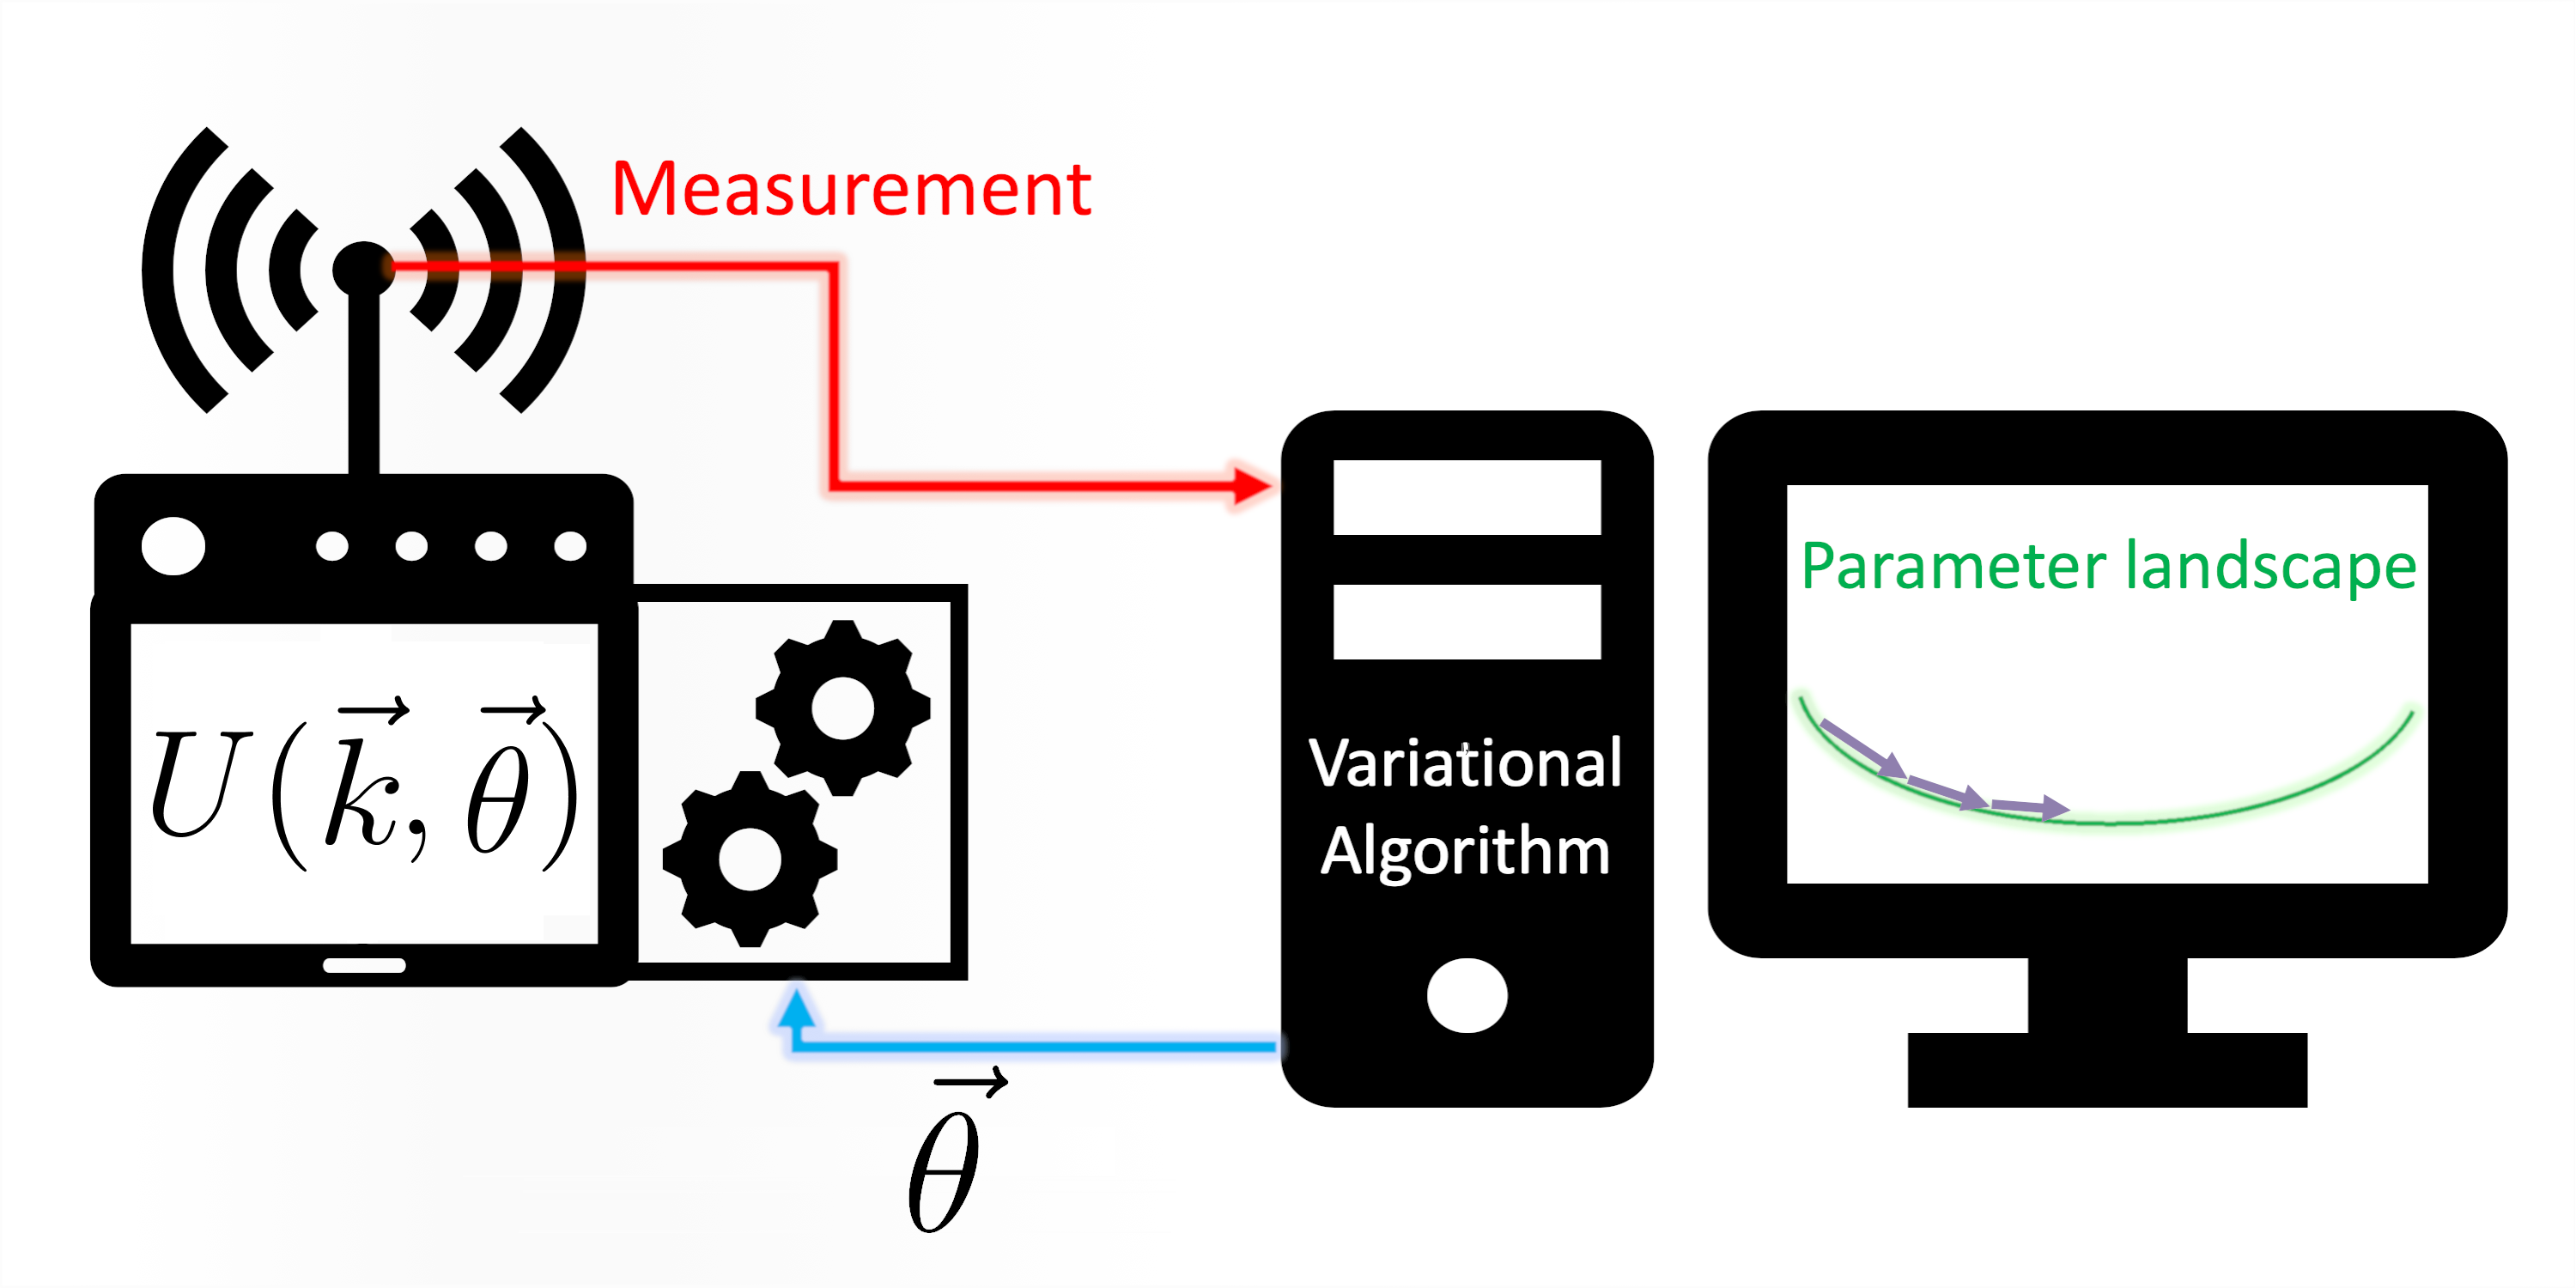
\includegraphics[width=1.\textwidth]{Figures/VANS/vqa_cycle.png}
    \caption{Figure adapted from Ref.~\cite{borrowed}: a generic VQA algortihm is sketched. Here, a quantum device is used to estimate a cost-function value, whereas the device itself is controlled by a classical optimization algorithm. This cycle is iterated until convergence.}
    \label{fig:VQAcycle}
\end{figure}
The estimation of a cost function via a quantum circuit and its modification (hopefully towards a cost-minimizing direction) by a classical optimization algorithm defines a cycle, which is repeated until convergence, as depicted in Fig.~\ref{fig:VQAcycle}. The success of such scheme hinges on several factors. As a matter of fact, the classical optimizer must be able to efficiently train the parameters, and in the past few years, there has been a tremendous effort in developing quantum-aware optimizers~\cite{verdon2018universal,kubler2020adaptive,arrasmith2020operator,stokes2020quantum,koczor2019quantum,nakanishi2020sequential,fontana2020optimizing}. In particular, severe trainability issues has been pointed out, which forbid the success of VQAs and as constitute the main barrer (along with hardware-noise) for making use of current NISQ devices in the VQA framework, and we will review some of them in Sec.~\ref{ssec:1_nisq_vans_bp}.

However, we note that even if such trainability issues could be overcomed, the performance of a VQA will intrinsically be linked to the specific quantum circuit used for the training. Here, the choice of an ansatz for $U(\kvec,\thv)$ plays a crucial role in determining the success of a VQA scheme; for instance, for a given Hamiltonian in the VQE algorithm, circuits that are close to the ground-state preparing one might lie outside the subspace $\mathcal{U}$ of the unitary group $U(n)$ which is generated by varying $\thv$ in $U(\kvec, \thv)$, with a fixed circuit layout given by $\kvec$~\cite{holmes2021connecting}.

In this respect, not every unitary transformation in $U(n)$ can straightforwardly be implemented, since the availability of quantum gates is often restricted; we generally need to deal with a \textit{gate-dictionary} $\mathcal{D}$, which in this thesis will be composed of one-qubit rotations and of CNOTs entangling any pair of qubits present in the circuit. We note that such an dictionary is universal~\cite{nielsen00}: any quantum gate can be implemented provided enough gates of the dictionary are used. Nevertheless, such a \textit{compilation} is a tricky one: noise accumulates with circuit's depth, and hence only a non-trivial set of unitaries can be reached. Moreover, we remark that the availability of fully-connected qubits is a slight simplification, and connectivity constraints should in principle be considered. In the latter case, entangling two qubits which are not straightforwardly connected represents an overhead in circuit's depth, and many efforts have been carried out recently in order to find novel strategies to tackle this issue~\cite{compilingDeepRLmaster}.

For these reasons, it is important to discuss different strategies ussually considered when constructing the quantum-circuit to be used in a VQA, also known as an \textit{ansatz}. %Here, we can readily distinguish between fixed-structure quantum circuits (where only the continuous paramters encoded in the rotations values are optimized), and variable-structure ones, in which both parameters \textit{and} strucure are optimized.


\subsection{The Ansatz}\label{ssec:1_nisq_vans_bp}
We refer to the \textit{ansatz} as the quantum-circuit structure, \textit{i.e.} the layout defining quantum-gates placements. While such a word stand for \textit{an educated guess or an additional assumption made to help solve a problem}~\cite{wikiansa}, let us remark that trainability and noise-related issues make it non-trivial to define what an \textit{educated guess} for a given problem is in the NISQ-era.

We will make a distinction between \textit{fixed}-structured ansatzes (\textit{i.e.} where $\kvec$ is fixed), and \textit{variable}-structure ones, in which also the structure of the circuit is optimized. In the latter case, the optimization is arguably more complex, since it consists on finding the right circuit structure on top of the continuous parameter optimization.

A key parameter that characterizes the ansatz is the number of gates present in the circuit. It is thus essential to construct ansatzes that maintain this number as low as possible to mitigate noise and trainability-related issues, but also that have enough expressibility to contain the problem solution (or at least an approximate version of it).

In the following we will first discuss some commonly-used fixed-structured ansatzes, and we will then turn to the variable-structure case.
% \subsubsection{Fixed-structure ansatzes}\label{sssec:blabla}

\vspace{1cm}

Let us now discuss on some commonly-used fixed-structure ansatzes. We first consider a \textit{separable} ansatz as depicted in Fig.~\ref{fig:FANSATZ}. Here, the structure is so trivial that no entanglement is generated by the circuit, since only local operations are performed on each qubit. Assuming that the initial state is separable ---we often consider it to be $\ket{0}^{\otimes n}$---, only a very small fraction of the Hilbert space can be reached under this circuit's choice~\cite{separableAnna}, and the overall performance is expected to be poor since the presence of entanglement is generally required. Also, note that the separable case can efficiently be simulated in a classical computer, and thus we do would not expect them to provide any quantum advantage.

\begin{figure}[t!]
    \centering
    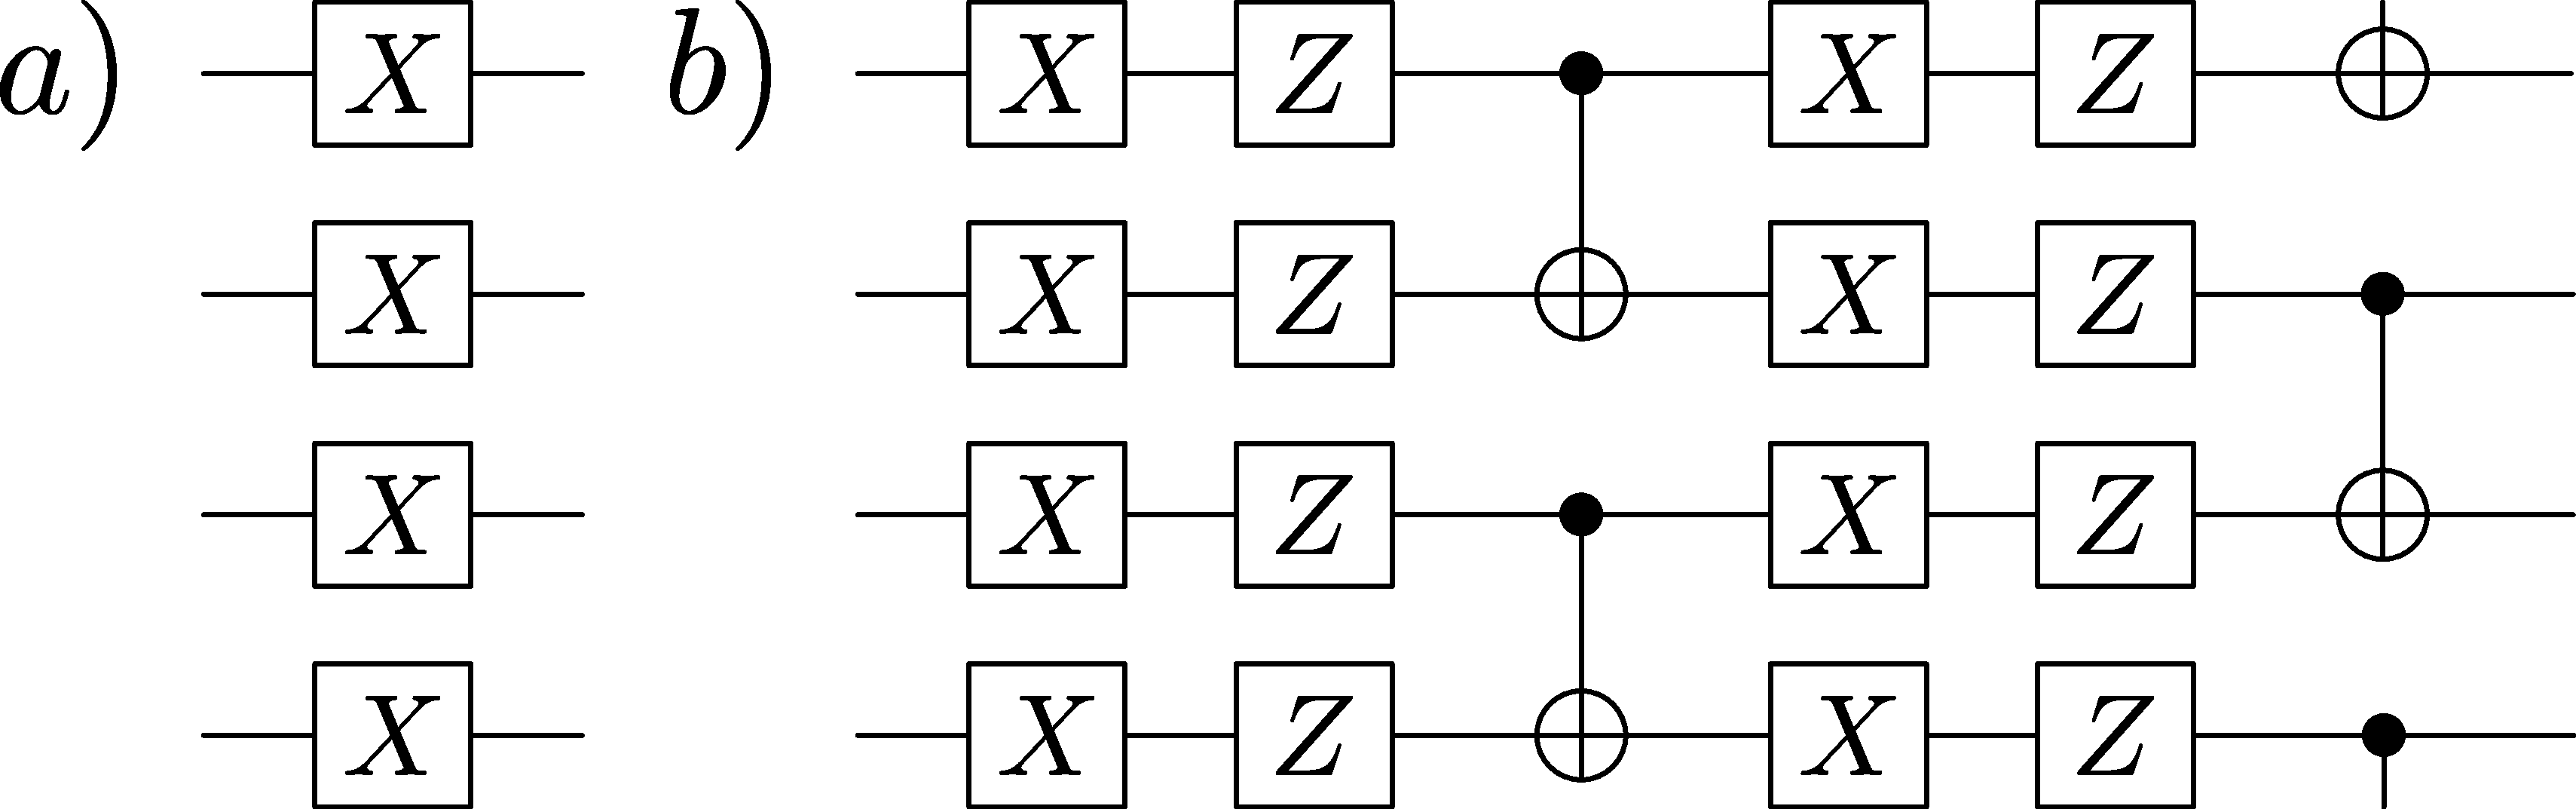
\includegraphics[width=1.\textwidth]{Figures/VANS/Fig2.pdf}
    \caption{We show examples of commonly-used quantum circuits. In \textit{(a)} we depict a separable product ansatz which generates no entanglement between the qubits. On the other hand, \textit{(b)} shows two layers of a shallow alternating Hardware Efficient Ansatz where neighboring  qubits are initially entangled.  Here $Z$ ($X$) indicates a parametrized rotation about the $z$ ($x$) axis (the angles $\bm{\theta}$ are not explicitely shown, but such are the degree of freedom to optimize over).}
    \label{fig:FANSATZ}
\end{figure}

This issue can be addressed with the layered Hardware Efficient Ansatz\cite{kandala2017hardware}, which we refer as HEA. Here, the gates are arranged in a brick-like fashion and act on alternating pairs of qubits, as depicted in Fig.~\ref{fig:FANSATZ}. We define a $L$-HEA as a circuit in which $L$ layers are stacked next to each other: a single layer consists on $n-1$ two-qubit gates (in the figure, rotations around $x$ and $z$ axis, followed by a CNOT) that correlate two neighbour qubits in the circuit. We here will consider the qubits as a cyclic chain, where the bottom one is also conected to the upper one, although this definition can be adapted to specific qubit-connection constraints of the quantum computer at hand. As $L$ increases, it can be expected that HEA becomes more expressible. as opposed to the separable circuit, whose expressibility is very poor.

In turn, HEA turns out to be \textit{too} expressible~\cite{holmes2021connecting}, in the sense that any unitary can be mimicked using enough HEA-layers, and this can lead to trainability issues. For a sufficiently-expressible PQC, the landscape of possible unitaries $\mathcal{U}$ that can be reached by varying its parameters turns to be hard to navigate, in the sense that the cost-function landscape becomes very flat, a phenomenon known as a \textit{barren plateau}. The latter fact constitute a big challenge for an optimization proccedure that needs to navigate such landscape and reach the lowest cost-function value, as discussed in Sec.~\ref{ssec:1_nisq_barrenplateaus}.

One of the main advantages of HEA is that it employs gates native to the specific device used, hence avoiding an unnecessary overhead in the number of gates present in the circuit, arising from compiling non-native unitaries into native gates (for instance, the building-blocks in the figure could be replaced with gates coming from another dictionary). This type of ansatz is \textit{problem-agnostic}, in the sense that it is expressible enough so that it can be generically employed for any task; in Chapter~\ref{chapter:VANS} we will often use this ansatz for benchmarking purposes.

On the other hand, a hint on the solution for the target problem to be solved by a quantum computer can, in principle, be helpful when building the ansatz. This claim should certainly holds in the ideal (\textit{e.g.} noise-less) scenario, and in VQAs, this is reflected by the so-called \textit{problem-inspired} ansatzes. Here the goal is to encode information of the problem into the ansatz's structure so the optimal solution of Eq.~\eqref{eq:optimization} exists within the parameter space without requiring high expressibility.

An example of such fixed-structure ansatzes is the Quantum Alternating Operator Ansatz (QAOA) for optimization problems, which is aimed to adiabatically prepare the ground-state of a \textit{problem}-hamiltonian, and thus alternates between a \textit{mixing} unitary and a \textit{problem} one. We will not discuss thse ansatzes here, and the interested reader can find more details in Refs.~\cite{farhi2014quantum,hadfield2019quantum}.

On a different note, considerable effort has been made in order to construct physically-inspired ansatzes in the field of quantum chemistry, and the Unitary Coupled Cluster (UCC) Ansatz~\cite{cao2019quantum,bartlett2007coupled} is an example of them. We will discuss the quantum-chemistry problem in greater detail in Sec.~\ref{ssec:molecular_ham_vans}. Essentially, we here seek to prepare the ground state of a molecular Hamiltonian, which (under the Born-Oppenheimer approximation) translates to solve a many-body fermionic system, known as the \textit{electronic-structure problem}.
While much insight from the classical methods that tackle this problem can be brought to the NISQ scenario, some issues raise up. Namely, we need to map the [UCC] ansatz from fermions to qubits, as well as the molecular Hamiltonian, since we are here targeting applications on digital quantum computers. Such mapping can be done by the Jordan-Wigner transform (or alternatively Bravi-Kitaev). Unfortunately, this ussually comes with an overhead in the number of quantum gates required to build the specific circuit (and also a large number of Pauli observables to represent the molecular Hamiltonian). This fact constitutes a big challenge for NISQ applications, since deep circuits are severely affected by noise.

We might think of quantum chemistry as a subset of problems that quantum computing can potentially addess. Generally, for a given physical problem, a family of quantum-circuit structures reflecting certain symmetries of potential solutions could in principle be constructed. However, quantum-hardware noise makes it highly no trivial to directly translate such physical intuition into the structure of the quantum circuit. %, since the afforementioned challenges related to noise generally arise.
\vspace{1cm}

Under the presence of limited resources, each component of the VQA that could in principle be optimized over, should be optimized over. This constitutes the spirit behind several efforts~\cite{grimsley2019adaptive,tang2019qubit,zhang2021mutual, rattew2019domain,chivilikhin2020mog, cincio2021machine, cincio2018learning,du2020quantum,zhang2020differentiable} to adapt the circuit layout to the specific scenario at hand (\textit{e.g.} a noise model, or the restricted availability of quantum hardware). In the following we will review some of such efforts, which are known as \textit{variable-structure ansatzes}. We remark that this is not the end of the story regarding optimization of VQA's components. As a matter of fact, we could also optimize the way cost-function estimates are obtained~\cite{algorithmiq1,algorithmiq2}, though we will only focus to optimizing circuit's structure.

The overall strategy of variable-structure ansatzes consists of iteratively changing the quantum circuit by placing (or removing) gates that empirically lower the cost-function value after the continuous-parameter optimization. The first proposal for variable ansatzes for quantum chemistry was introduced in~\cite{grimsley2019adaptive} under the name of ADAPT-VQE. Here, the authors follow a circuit structure similar to that used in the UCC ansatz introduced above, and propose to iteratively grow the circuit by appending gates that implement fermionic operators chosen from a pool of single and double excitation operators. At each iteration, one decides which operator in the pool is to be appended, which can lead to a considerable overhead if the number of operators in the pool is large. Similarly to the UCC case, the mapping from fermions to qubits can lead to prohibitively deep circuits. This issue can be overcomed using the qubit-ADAPT-VQE~\cite{tang2019qubit} algorithm, where the pool of operators is modified in such a way that only easily implementable gates are considered. However, the size of the pool still grows with the number of qubits. We refer the reader to~\cite{claudino2020benchmarking} for a detailed comparison between ADAPT-VQE and UCC ansatzes.

A different approach to variable-structure ansatzes that has gained considerable attention are machine-learning-aided evolutionary algorithms (EA) that upgrade individuals (quantum circuits) from a population. Noticeably, the presence of quantum correlations makes it so that it is not straightforward to combine features between circuits during the evolution, as simply merging two promising circuits does not necessarily lead to low cost-function values. Thus, only random mutations have been considered so far. An example of this method is found in the
Evolutionary VQE (EVQE)~\cite{rattew2019domain}, where one explores the Hilbert space \textit{smoothly} by growing the circuit with identity-initialized blocks of gates and randomly removing sequences of gates. Another example of an evolutionary algorithm is the Multi-objective Genetic VQE (MoG-VQE)~\cite{chivilikhin2020mog}, where one uses building blocks that are randomly placed along the circuit, and simultaneously optimizes both the energy and number of entangling gates. Evolutionary algorithms constitute a promising approach to ansatzes design, they nevertheless come at the cost of high quantum-computational resources to evolve populations of quantum circuits.

In addition, in Refs.~\cite{du2020quantum,zhang2020differentiable,pirhooshyaran2021quantum,du2020quantum} tools from auto-machine were employed in order to learn how to build ansatzes. The overall idea behind these methods is that of employing neural network (supernet) that suggests the quantum circuit structure; supernet-training can be done using policy-gradient methods, a variant of the reinforcement-learning algorithms that we consider in Sec.~\ref{sec:1_rl}. While the idea of artificial-intelligence improving (quantum) neural-network architectures is exciting, it is extremely resource-consuming: recall that the amount of data required to train a neural network is very often prohibitively high. Similarly to the EA case, the high amount of resources consumed by this method is a challenge that needs to be addressed.

Finally, in Refs.~\cite{cincio2018learning,cincio2021machine} a methodology, formalized by the VAns algorithm~\cite{bilkis2021semi} --- \textit{i.e.} our main contribution to the field, and explained and showcased in great detail in Chapter~\ref{chapter:VANS} --- was used to obtain a short-depth version of a given unitary under specific quantum hardware constraints (such as connectivity, noise-model as represented by quantum channels or available gates). %Explaining and showcasing our algorithm will be the matter of Chapter~\ref{chapter:VANS}.

Having reviewed some commonly-used quantum circuit structures, we will now turn to discuss the continuous optimization.


\subsection{The optimization procedure}\label{ssec:optimizer}
With a quantum circuit parametrized by $U(\kvec,\thv)$, VQAs employ a classical optimization algorithm in order to minimize the cost-function in Eq.~\eqref{eq:cost}. Here, we will focus on derivative-based methods, which at each cycle $\ell$ of the algorithm, the gradient $\nabla _{\thv} C(\kvec,\thv)$ is computed, and a cost-minimizing direction is followed. Ussually, the initial parameters $\thv^{\ell}$ are randomly chosen (this random initialization should be understood according to the Haar measure, as we discuss in the next Section). In the following we will first discuss about optimization algorithms, and then on how such gradients can be computed.

The most straightforward approach in gradient-based optimization is that of following the gradient; as such we are guaranteed to attain (at least) a local minima. Thus, in Gradient Descent algorithm, the continuous parameters are updated according to
\begin{equation}\label{eq:GD}
\thv^{(\ell + 1)} = \thv^{(\ell)} - \alpha \nabla _{\thv}(\kvec,\thv)|_{\thv = \thv^{(\ell)}},
\end{equation}
where $\alpha$ is the \textit{learning-rate}, accounting for the update-step size, and this is guaranteed to reach, at least, a local-minima.

In optimization problems where the dataset is too large, computing the gradients can be prohibitively expensive (for instance, if the entire dataset does not fit in the memory). In this case, the training set is splitted into chunks, and an stochasticity arises when estimating gradient; such is the case of Stochastic Gradient Descent (SGD), where the gradient is estimated out of $b$-dimensional data subsets known as \textit{batches}. At each cycle, the data is randomly splitted and the update rule of Eq.~\ref{eq:GD} is sequentially applied using the gradient $\nabla _{\thv} C(\kvec,\thv)$ computed using each batch (note that this injects stochasticity); an \textit{epoch} is consequently defined as an entire pass of the original training set. We note that this stochasticity, which might in principle appear undesired, it can actually be helpful since taking random directions often help in escaping local minima.

While a large learning-rate value in Eq.~\ref{eq:GD} can potentially forbid the optimizer to reach the actual minima (since the update becomes simply \textit{too large}), we note that small learning-rate values will potentially dampen the convergence rate. More elaborate optimization algorithms can be considered, which adapt the magnitude of the learning-rate according to the gradient landscape at hand. Among them, a very popular optimizer is the Adaptive Moment Estimation (Adam) algorithm~\cite{kingma2015adam}, which sequentially adapts the learning rate for each parameter, by specifically tailoring it out from moving averages of first and second moments for each gradient component. In practice, this allows to reach a better optimization performance, although we shall ultimately adapt the optimization algorithm to the specific problem at hand. In the context of VQA, many issues need to be addressed, such as shot-noise, sampling-complexity and optimal choice of learning-rate values to take into account the quantum nature of the optimization landscape; in this regard there has been a tremendous effort in developing quantum-aware optimizers~\cite{verdon2018universal,kubler2020adaptive,arrasmith2020operator,stokes2020quantum,koczor2019quantum,nakanishi2020sequential,fontana2020optimizing,gu2021adaptive}.

With a basic understanding on how optimization algorithms proceed, let us now discuss how the essential ingredient in the update-rule can be obtained under the VQA framework. For this, we distinguish between two approaches: \textit{(i)} classical simulation of quantum circuits, and \textit{(ii)} experimental implementations on quantum hardware.

\subsubsection{Classical simulation of quantum circuits $\&$ Automatic differentiation}
If no particular symmetries are imposed, we are able to simulate quantum systems classically for up to $\sim 30$ qubits\footnote{On the contrary, many systems can be approximated efficiently by using clever ansatzes; this lies at the heart of Tensor Network (TN) methods such as Matrix Product States (MPS), Density Matrix Renormalization Group (DMRG) or Multiscale Entanglement Renormalization Ansatz (MERA). There is currently much excitement about TNs: while the space of all possible quantum states is large, only a portion of it is \textit{physically relevant} and it is believed that such portion can be simulated efficiently using TNs~\cite{Biamonte2017tensornetworks,orusTN}.}.
%
State-of-the-art techniques used to classically compute VQA-cost-function gradients rely on automatic differentiation (AD), in which cost-function derivatives are obtained by tracking each intermmediate-operation derivative, and following the chain-rule~\cite{broughton2020tensorflow,Luo2020yaojlextensible}. This is done by decomposing a generic program in terms of elementary operations whose derivatives can be computed, and is the spirit behind the paradigm of \textit{differentiable programming}~\cite{Rackauckas2020GeneralizedPL,Liao2019differentaible,dpcontrolsto}.

We remark that AD differs from numerical differentiation (such as finite differences) since it is an exact method. Similarly to symbolic differentiation, each operation involved in the computation provides a rule for its derivative with respect to the corresponding input. However, the output of AD is a numerical value of the derivative, and not a mathematical expression for it.

In turn, AD is carried out by constructing a \textit{computational graph}, where nodes are associated to the elementary operations present in the computation (and whose derivatives are known), and where the dependence on the parameters is explicited. In order to compute the function derivative, the graph is transversed either forward or backwards; the latter case is known as \textit{backpropagation}\footnote{The optimal way to transverse the computational graph generally depends on the setting at hand. For high-dimensional inputs (as customary when working with neural networks), backpropagation is prefered at the cost of an increase in memory usage.}. Thanks to efficient matrix multiplication sub-routines and special-purpose hardware such as GPUs and TPUs, this can be done consideraly fast, and in turn AD stands as one of the main ideas behind the advent of Artificial Intelligence.

\begin{figure}[t!]
    \centering
    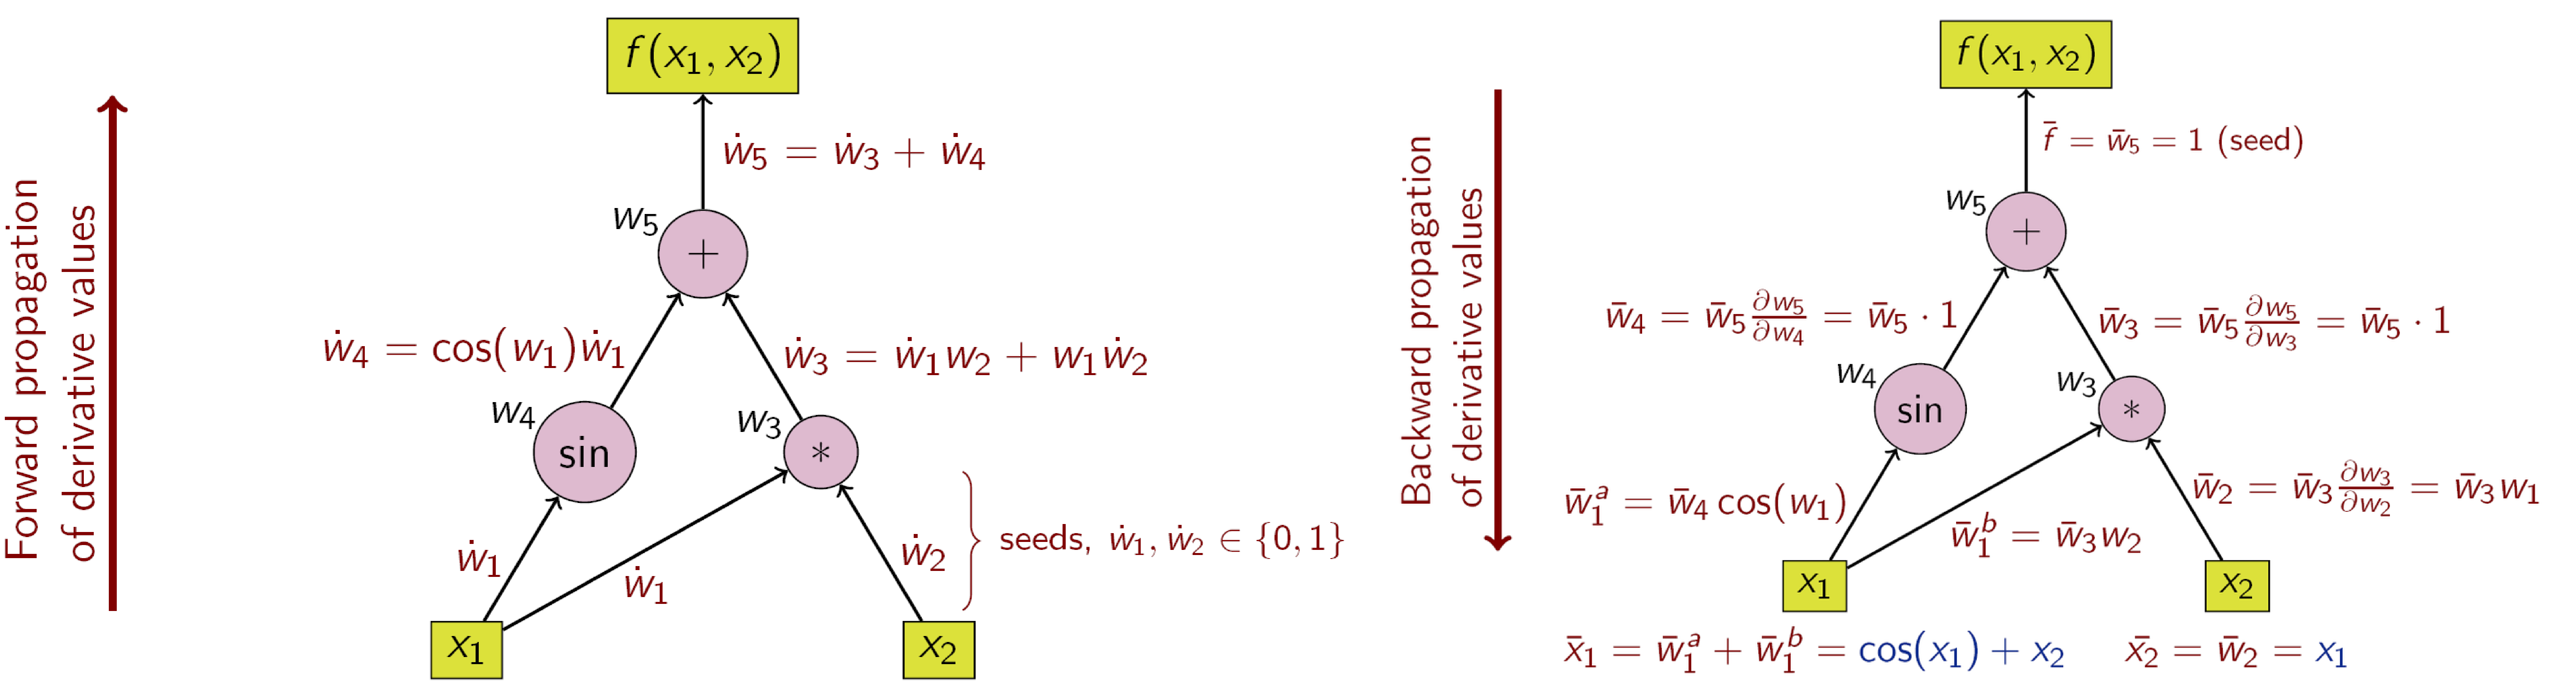
\includegraphics[width=1.\textwidth]{Figures/ad.pdf}
    \caption{We show how the computational graph is travelled forward and backwards in each of the possible modes of AD, for the example of an scalar function $f(x_1,x_2) = x_1 x_2 + \sin(x_1)$}
    \label{fig:ad}
\end{figure}

Let us consider an example\footnote{Taken from Ref.~\cite{wikiAD}} of an algorithm taking as input a real-value $x$, and outputing $y = f(g(h(x))$ where $f,g$ and $h$ are elementary functions whose derivatives are well-known and can be recorded when building the computational graph. We aim to compute $\partial_x y$, and to this end we define $w_0 = x$, $w_1 = h(w_0)$, $w_2 = g(w_1)$ and $w_3 = f(w_2) = y$. Now, the chain rule implies that
\equ{\frac{\partial y}{\partial x} = \frac{\partial y}{\partial w2} \frac{\partial w2}{\partial w1}  \frac{\partial w1}{\partial x}.} Thus, the computational graph is built by recording each of the elementary functions that need to be computed \textit{and} each of the elementary functions derivatives, which are known in advance. Then, forward-AD transverses the chain-rule from inside to outside, by first computing $\frac{\partial w_1}{\partial x}$, then $\frac{\partial w_2}{\partial w_1}$ and finally $\frac{\partial y}{\partial w_2}$.
On the contrary, backwards-AD transverses the chain-rule from outside to inside, by first computing $\frac{\partial y}{\partial w_2}$, then $\frac{w_2}{w_1}$ and finally $\frac{\partial w_1}{\partial x}$. As a concrete example, we can consider the function
\begin{align}
y &= f(x_1, x_2) \\
&= x_1 x_2 + \sin(x_1) \\ 
&= w_1 w_2 + \sin(w_1) \\
&= w_3 + w_4 \\
&= w_5,
\end{align}
where at each elementary operation we define a new variable $w_i$, which represents a node in the computational-graph. In the table we show the operations needed to compute the function, forward-AD, and backward-AD (this is also schematised in Fig.~\ref{fig:ad}).
\begin{center}
\begin{tabular}{| c |c |c |}
\hline
Function computation  &  Forward-AD&  Backward-AD\\
\hline
  $w_1 = x_1$&  $\dot{w}_1 = 1$ (\texttt{seed})&  $\bar{w}_5 = 1$ \texttt{seed}\\
  \hline
  $w_2 = x_2 $&  $\dot{w}_1 = 0$ (\texttt{seed})&  $\bar{w}_4 = \bar{w}_5 \cdot 1$\\
  \hline
  $w_3 = w_1\cdot w_2$& $\dot{w}_3 = \dot{w}_1\cdot w_2+ w_1 \cdot \dot{w}_2$ &  $\bar{w}_3 = \bar{w}_5 \cdot 1$\\
  \hline
  $w_4 = \sin(w_1)$& $\dot{w}_4 = \cos(w_1)\cdot \dot{w}_1$  &  $\bar{w}_2 = \bar{w}_3 \cdot w_1$\\
  \hline
  $w_5 = w_3 + w_4$& $\dot{w}_5 = \dot{w}_3 + \dot{w}_4$ &  $\bar{w}_1 = \bar{w}_3 \cdot w_2 + \bar{w}_4 \cos(w_1)$\\
  \hline
\end{tabular}
\end{center}
Here, we used the notation of $\bar{w}_i=\frac{\partial y}{\partial w_i}$ for the backward-AD, and note that the \textit{seed value} in this example is trivial for such case (since it stands for possible multidimensional outputs, \textit{e.g.} cases where $y \in \mathbb{R}^n$). On the contrary, since the example function has two inputs $(x_1, x_2)$, forward-AD needs to be specified which derivative we are computing ---either $\partial_{x_1} y$, as set by the seed value in the table, or $\partial_{x_2} y$---. Note that to compute the gradient, we would need two passes of the graph for this example\footnote{For a vector field $f:\mathbb{R}^m\rightarrow \mathbb{R}^n$, then computing the gradient requires $m$
computational graphs sweeps for the backward-AD, and $n$ sweeps for the forward-AD.}.

While this discussion only provides an introduction to the meaning of AD, we remark that much work has been done in this field during the last years, and we refer the interested reader to Refs.~\cite{wikiAD,abadi2016tensorflow,maclaurinautograd,maclaurin2016phd,survey_ad}.

\subsubsection{Experimental implementations on quantum hardware}
In NISQ circuits, backpropagating cost-function derivatives imply that the quantum state at each step in the circuit should be kept in memory, a fact essentially forbiden because of exponentially large Hilbert-spaces. Alternatively, we can use quantum hardware to compute such gradients.

In this scenario, cost-function derivatives can be obtained by the so-called \textit{parameter-shift rules} where cost-function derivatives are expressed as linear combinations of cost-function values, each obtained by using the very same circuit, but shifting the parameters by a finite amount. We remark that this is an analytic result, unrelated to numerical differentiation techniques such as finite differences\footnote{In turn, finite-differences do not get along with gradient-based optimizers, and often leads to inestabilities due to approximation errors; this issue intensifies in the NISQ framework, since we generally need to resolve between cost-function values that are small. Estimating such difference in cost-function values turns difficult, since not only a high amount of samples is required, but also the strong presence of hardware-noise can potentially forbid to resolve it.}.

In the following we will detail the idea behind parameter-shift rules. Let us consider a single parameter $\alpha \in \thv$, and a VQE problem, whose Hamiltonian is $\hat{H}$ and thus the cost-function becomes %(see also Eq.~\ref{eq:vqe_cost})
\begin{equation}
C(\thv) = C_{\text{VQE}}(\thv)= \expect{0|U^\dagger(\thv) \hat{H}U(\thv)|0},
\end{equation}
where we momentaneaously simplified our notation by dropping the dependence on $\kvec$, and used the notation $\ket{0}^{\otimes n} \equiv \ket{0}$).

Moreover, we will assume that $U(\thv) = U_L G(\alpha) U_R$, where $U_L$ and $U_R$ are unitary transformations parametrized by $\thv - \llaves{\alpha}$. Upon defining $\ket{\psi} = U_R \ket{0}$, and $\hat{Q} = U_L^\dagger \hat{H}U_L$, it follows that
\begin{align}\label{eq:shifted}
\partial_\alpha C(\thv) =& \expect{\psi |G^\dagger \hat{Q} (\partial_\alpha G)| \psi} + \expect{\psi |(\partial_\alpha G^\dagger) \hat{Q} \partial_\alpha G| \psi},\end{align}
where we used $G$ as a shorthand for $G(\alpha)$. Now, let us consider $G(\alpha) = e^{-\ii \frac{\alpha}{2} P}$, %$ = \cos(\frac{\alpha}{2}) - \ii \sin(\alpha) P$,
with $P \in \llaves{\sigma_x, \sigma_y, \sigma_z}$. In this case, we obtain
\begin{align}
\partial_\alpha C(\thv) =& \frac{\ii}{2}\expect{\psi |G^\dagger \Comm{P}{\hat{Q}} G |\psi}.\end{align}
Now, using the following identity, which holds for any operator $\sigma$~\cite{shiftrules1}:
\equ{\Comm{P}{\sigma} = \ii \Big( G(\frac{\pi}{2}) \sigma G(-\frac{\pi}{2}) - G(-\frac{\pi}{2}) \sigma G(\frac{\pi}{2}) )\Big),}
we get
\begin{align*}
\partial_\alpha C(\thv) =& -\frac{1}{2}\Big(\expect{\psi |G(\alpha)^\dagger G^\dagger(-\frac{\pi}{2}) \hat{Q} G(-\frac{\pi}{2}) G(\alpha)|  \psi}  + \expect{\psi |G(\alpha)^\dagger G^\dagger(\frac{\pi}{2}) \hat{Q} G(\frac{\pi}{2}) G(\alpha)|  \psi} \Big)
\end{align*}
By noting that $G(\alpha)G(\beta) = G(\alpha + \beta)$, and recalling that $\hat{Q} = U_L^\dagger \hat{H}U_L$, it follows that
\begin{equation}\label{eq:der}
\partial_\alpha C(\thv) = \frac{1}{2}\big(C(\thv)|_{\alpha \leftarrow \alpha + \frac{\pi}{2}} - C(\thv)|_{\alpha \leftarrow \alpha - \frac{\pi}{2}}\big)
\end{equation}
This procedure can be extended to consider arbitrary Pauli strings~\cite{shiftrules1}, and unitary transformations for which the derivative is not unitary. In the latter case, the derivative can be written as a linear combination of unitary operations, resulting in a generalized parameter-shift rule which --- as opposed to Eq~\ref{eq:der} --- involves more than two contributions~\cite{shiftrules2, Wierichs2022generalparameter}.

Thus, the cost-function derivatives can be obtained by estimating each term in Eq.~\ref{eq:der} using a quantum computer parametrized by $U(\thv)$, and repeating this procedure for each parameter $\alpha \in \thv$. As mentioned, this result is exact (contrary to numerical differentiation methods); it nevertheless relies on cost-function estimates, thus statistical fluctuations arising from measurement outcomes will always be present. This plays an important role if the value of such derivatives is small, in which case many measurements will be required in order to deal with sufficient accuracy.

Thus, VQAs' optimizers will generally need to deal with an intrinsically stochastic component, and convergence properties of SGD has been analyzed in Ref.~\cite{Sweke2020}. Following such reference, we can readily distinguish between different sources of \textit{stochasticity}, the first one being shot-noise. Alternatively, in Eq.~\ref{eq:decoH} we have decomposed the Hamiltonian as a sum of Pauli-string, and at each cycle of the optimization algorithm, the gradient could be estimated out of a subset of all the Pauli strings present in such decomposition. In this case, another source of stochasticity arises, and is associated to estimating cost-function gradient out of a subset of terms appearing in the cost-function. Methods combining both techniques are known as \textit{doubly-stochastic} optimizers~\cite{Sweke2020,harrow2019low}.

Overall, parameter-shift rules can be understood as a \textit{recipe} for computing gradients of cost functions; we remark that the approach presented above naturally generalizes to cost-functions of the form in Eq.~\ref{eq:cost}. Under this recipe, circuit's structure needs not to be modified, but rather the parameter in question is shifted, and the derivative is obtained as linear combination of the corresponding cost-function estimates. For classical simulation purposes, the \textit{best of both worlds} are ussually combined, and backpropagation methods are used along with the parameter-shift rules (provided that the systems under consideration are not too large); this is one among the many efforts behind projects like TensorFlow-Quantum or PennyLane ~\cite{bergholm2018pennylane,broughton2020tensorflow}.

By now, we have introduced the basic ingredients required to run a VQA. Namely, a strategy that defines the structure of our quantum circuit, a cost-function that evaluates its performance, and a (classical) optimization algorithm that takes control of free parameters such as rotation values. The ultimate goal is to find the global minima of the cost function by navigating the optimization landscape. In this regard many issues have been recently raised up, which put into question the overall feasibility of VQA framework, and that is the matter of our next section.


\subsection{Barren-plateaus}\label{ssec:1_nisq_barrenplateaus}
The barren plateau (BP) phenomenon has recently received considerable attention as one of the main challenges to overcome for the VQA framework to provide a quantum speedup. BPs refer to the exponentially vanishing (in the number of qubits) for a random circuit to present a gradient component which is slightly higher than zero. In turn, this constitutes a big challenge when navigating the cost-function landscape, since such landscape (\textit{e.g.} the set of unitaries that are generated when varying the parameters of a sufficiently random PQC) becomes flat in the pressence of a BP.

In the following we will first outline how the BP phenomenon emerges from a 2-design, and then discuss several extensions of this phenomena to other classes of circuits.

\vspace{1cm}

The notion of $t$-design quantifies how similar the measure obtained from varying parameters $\thv$ in $U(\kvec, \thv)$ differs from that of the Haar measure, which is the uniform measure in $U(n)$. A random event refers to randomly sampling an unitary transformation from $\mathcal{U}$, \textit{i.e.} the set of unitaries that are generated from $U(\kvec, \thv)$ by modifying the parameters $\thv$. Thus, we can define an expressibility super-operator as
\equ{\mathcal{A}^{(t)}_\mathcal{U}(\cdot) = \int_{\mathcal{U}} d_\mu(U)\; U^{\otimes t} (\cdot) {U^\dagger}^{\otimes t} - \int_{U(n)} d_{\mu_H}(U) \;U^{\otimes t} (\cdot) {U^\dagger}^{\otimes t},}
where $d_{\mu_H}(U)$ denotes the volume element of the Haar measure, and $d_\mu(U)$ is the volume element corresponding to the uniform distribution over $\mathcal{U}$~\cite{holmes2021connecting}; for PQCs such set is generated by uniformly sampling over the parameters $\thv$.

Thus, $\mathcal{U}$ forms a $t$-design if $\mathcal{A}^{(i)}(X) = 0$ for every operator $X$ and every $i=1,...,t$, meaning that the uniform distribution over $\mathcal{U}$ matches the uniform distribution over $U(n)$ up to the first $t$-moments. Using some useful identities from integrating over the Haar measure, namely that
\begin{align}\label{eq:relations_haar}
\int_{U(n)} d_\mu(U) \; U_{ij} U^{*}_{mk} =& \frac{\delta_{im}\delta_{jk}}{n} \\
\int_{U(n)} d_\mu(U) \; U_{ij} U_{kl} U^*_{mn} U^*_{op}  =& \frac{1}{n^2-1}(\delta_{im} \delta_{jn} \delta_{ko} \delta_{np} + \delta_{io} \delta_{km} \delta_{jp} \delta_{ln}) \\ & -\frac{1}{n(n^2-1)}(\delta_{i m} \delta_{ko} \delta_{jp} \delta_{ln} + \delta_{io} \delta_{km} \delta_{jn} \delta_{lp}), \nonumber
\end{align}
the landscape of $2$-designs was explored in Ref.~\cite{mcclean2018barren}. In particular, using the identities we can show that 2-designs have gradients which are on average (over the Haar measure) zero-valued, which indicate that the landscape is not \textit{biased} towards any particular direction. Moreover, the identities can also be used to compute the variance of the cost-function gradient, and the result (for $2$-designs) is that it exponentially vanishes with the number of qubits present in the circuit:
\begin{equation}\label{eq:BP}
    \Var\left[\partial _\alpha C_{\text{VQE}}(\kvec,\thv)\right]\leq F(n)\,, \quad \text{with} \quad F(n)= \OC\left(\frac{1}{2^n}\right)\ ,
\end{equation}
where $\alpha\in\thv$. From Chebyshev's inequality we have that $\Var\left[\partial _{\alpha} C(\kvec,\thv)\right]$ bounds the probability that the cost-function partial derivative deviates from its mean value (of zero) as
\begin{equation}\label{eq:Chebyshev}
    \Pr\left[\left|\partial_\alpha C(\kvec,\vec{\theta})\right|\geq c\right]\leq\frac{\Var[\partial_\alpha C(\kvec,\vec{\theta})]}{c^2} \sim \mathcal{O}(2^{-n}),\,,
\end{equation}
for any $c>0$. This indicates that when navigating the set $\mathcal{U}$ by varying parameters $\thv$, an optimizer will observe a considerably flat landscape with a high probability. Here, such probability is associated to the chances that, after a random circuit initialization, the cost-function value associated to such circuit presents a gradient whose value is larger than $c$, as per Eq.~\ref{eq:Chebyshev}.

Thus, two difficulties arise when using a quantum computer in this context.

On the one hand, we will need to deal with shot-noise arising from meaurements done to estimate the cost-function value. Here, the accuracy of the estimations is proportional to the squared-root-inverse of the number of shots $N$.

On the other hand, navigating through the set $\mathcal{U}$, \textit{i.e.} the set of unitary transformations that can be reached from the parametrized quantum circuit under consideration $U(\kvec,\thv)$, when varying the continuous parameters $\thv$. Here, the probability of reaching a higher-than-$\epsilon$ gradient in Eq.~\ref{eq:Chebyshev} should be understood in terms of the parameter landscape: high gradients are exponentially unlikely to be reached, when randomly varying the parameters. Nevertheless, the optimizer will ultimately need to deal with such small gradients, and for the optimization procedure not to behave like a random-walk, we will need to resolve between this gradients, and the accuraccy required to accomplish that will generally require a high number of measurements~\cite{mcclean2018barren}. In this sense, exponentially many resources will be required to navigate such flat landscape.


While barren plateaus were first identified for large circuits, they were shown to be present in shallow circuits as well. Here, cost-function locality plays a crucial role: while several choices of observables $\{O_i\}$ and functions $\{f_i\}$ can lead to different faithful cost functions (\textit{i.e.}, cost functions whose global optima correspond to the solution of the problem), global cost functions can lead to trainability issues for large problem sizes~\cite{cerezo2020cost,sharma2020trainability}. Here we recall that global cost functions are defined as ones where $O_i$ acts non-trivially on all $n$ qubits. On a different note, the BP-phenomena discussed above has so-far considered 2-designs. In this sense, Refs.~\cite{holmes2021connecting,larocca2021diagnosing} study the presence of BPs when the circuits are $\epsilon$-close to a 2-design. In particular, the expressibility of a quantum circuit (\textit{i.e.}, which sample large regions of the unitary group~\cite{sukin2019expressibility}), can be linked to the amount of entanglement it generates~\cite{sharma2020trainability,patti2020entanglement,marrero2020entanglement}, which serves as a tool to diagnosticate the presence of a BP. For example, the Hardware-Efficient-Ansatz is a highly expressible circuit, and consequently suffers from an expressibility-induced BP. Several promising strategies have been proposed to \textit{mitigate barren plateaus}, such as correlating parameters~\cite{volkoff2021large}, layerwise training~\cite{skolik2020layerwise}, and clever parameter initialization~\cite{grant2019initialization,verdon2019learning}. Nonetheless, constructing smart ansatzes that do not present BPs seem to be the most promising route to avoid them; an example of such are the Quantum Convolutional Neural Networks~\cite{Cong2019,pesah2020absence}.

However, this is not the end of the barren-pleateu story: there exists a second effect that leads to barren plateaus which can even affect smart ansatzes with no randomness or entanglement-induced barren plateaus. As shown in Ref.~\cite{wang2020noise}, the presence of certain noise models acting throughout the circuit maps the input state toward the fixed point of the noise model (\textit{i.e.}, the maximally mixed state)~\cite{wang2020noise,franca2020limitations}, which effectively implies that the cost function value concentrates exponentially around its average as the circuit depth increases. Explicitly, in a noise-induced barren plateau (NIBP) we now find that
\begin{equation}\label{eq:NIBP}
    \left|\partial _{\alpha} C(\kvec,\thv)\right|\leq g(n)\,, \quad \text{with} \quad g(L)= \OC\left(\frac{1}{q^L}\right)\,,
\end{equation}
where $q>1$ is a noise parameter and $L$ the number of ansatz's layers. From Eq.~\ref{eq:NIBP} we see that noise-induced barren plateaus will be critical for circuits whose depth scales (at least linearly) with the number of qubits. It is worth remarking that Eq.~\ref{eq:NIBP} is no longer probabilistic as the whole landscape flattens. Here, we note that strategies aimed at reducing the expressibility of the circuit cannot generally prevent the cost from having a noise-induced barren plateau, since here reducing the circuit noise (\textit{e.g.} improving the quantum hardware) and employing shallow circuits seem to be the only viable and promising strategies to prevent these barren plateaus at the moment.


\subsection{Discussion}\label{ssec:1_nisq_discu}
In this Chapter, we have introduced the VAns algorithm, a semi-agnostic method for building variable-structure parametrized quantum circuits.

At each iteration of the optimization, VAns stochastically grows the circuit to explore the architecture hyperspace. Crucially, VAns also compresses and simplifies the circuit by removing redundant and unimportant gates. This is a key aspect of our method, as it differentiates VAns from other variable ansatz approaches and allows us to produce shallow circuits, which can potentially mitigate the effect of noise.

To showcase the performance of VAns, we simulated our algorithm for several paradigmatic problems in the so-called quantum machine learning framework. Namely, we implemented VAns to find ground states of condensed matter systems and molecular Hamiltonians, for a quantum autoencoder problem and for 10-qubit QFT compilation. In all cases, VAns was able to satisfactory create circuits that optimize the cost. Moreover, due to VAns' specific circit-compression rules, these optimal circuits contain a small number of trainable parameters and entangling gates. Here we also compared the result of VAns with those obtained by using a Hardware Efficient Ansatz with either the same number of entangling gates or the same number of parameters: in all cases we found that VAns could achieve the best performance. This point is crucial for the success of VAns in the presence of noisy channels, as it automatically adapts the circuit layout to the situation at hand (\textit{e.g.} noise strength). For instance, under the $\lambda$-model (which is the noise model we have proposed and implemented), VAns notably outperforms HEA under ground-state preparation tasks.

While we provided the basic elements and structure of VAns (\textit{i.e.}, the gate \texttt{Insertion} and gate \texttt{Simplification}  rules), these should be considered as blueprints for variable ansatzes that can be adapted and tailored to more specific applications. For instance, the gates that VAns inserts can preserve a specific symmetry in the problem. Moreover, one can cast the VAns architecture optimization (\textit{e.g.}, removing unimportant gates) in more advanced learning frameworks. Examples of such frameworks include supervised learning~\cite{supercomi} or reinforced learning schemes~\cite{foselgoogleRL,Moro2021,HerreraMarti2022policygradient}, which could potentially be employed to detect which gates are the best candidates for being removed.

We expect VAns to be especially useful for abstract applications, such as linear systems~\cite{bravo2020variational,huang2019near,xu2019variational}, factoring~\cite{anschuetz2019variational}, compiling~\cite{khatri2019quantum,sharma2019noise}, metrology~\cite{beckey2020variational,koczor2020variational}, and data science~\cite{larose2019variational,cerezo2020variational,biamonte2017quantum,schuld2014quest,abbas2020power,verdon2019quantum}, where physically motivated ansatzes are not readily available. In addition, VAns will likely find use even for physical applications such as finding grounds states of molecular and condensed matter systems, as it provides an alternative to physically motivated ansatzes for mitigating the impact of noise, as shown in our noisy simulations. This is particularly promising since we have seen that VAns readily adapts the ansatz to the noise situation at hand.

Let us now discuss how VAns is expected to deal with barren pleateaus, which currently constitute one of the major barriers for the success of VQA frameworks.

\subsection{Mitigating the effect of barren plateaus}
% Let us now discuss why VAns is expected to mitigate the impact of barren plateaus.
First, consider the type of BPs that are caused by the circuit approaching an approximate 2-design~\cite{mcclean2018barren}. Approximating a 2-design requires a circuit that both has a significant number of parameters and also has a significant depth~\cite{brandao2016local,dankert2009exact,harrow2009random,harrow2018approximate,haferkamp2022randomquantum}. Hence, reducing either the number of parameters or the circuit depth can combat the appearence of barren plateaus. VAns attempts to reduce both the number of parameters and the depth and consequently attempts to avoid approximating a $t$-design.

Second, consider the BPs that are caused by hardware noise~\cite{wang2020noise}. For such barren plateaus, it was shown that the circuit depth is the key parameter, as the gradient vanishes exponentially with the depth. As VAns actively attempts to reduce the number of CNOTs, it also reduces the circuit depth. Hence VAns will mitigate the effect of noise-induced barren plateaus by keeping the depth shallow during the optimization. As we have seen in our noisy simulations in Sec.~\ref{ssec:vans_results_noise}, VAns automatically adjusts the circuit layout in such a way that the cost function reaches a minima, which translates to short-depth circuits in noisy scenarios.

\subsection{Future directions}

\subsubsection{BP-aware implementation}
While in the previous subsection we have presented general arguments as to why VAns can improve trainability, here we instead present a practical method that combines VAns with the recent techniques of Ref.~\cite{sack2022avoiding} for mitigating barren plateaus using classical shadows.

As discussed in Sec.~\ref{ssec:1_nisq_barrenplateaus}, it is known that the presence of barren plateaus is intrinsically related to the entanglement generated in the circuit~\cite{sharma2020trainability,patti2020entanglement,marrero2020entanglement}. That is, circuits generating large amounts of entanglement are prone to barren plateaus. With this remark in mind, the authors in~\cite{sack2022avoiding} propose to detect the onset of a barren plateau by monitoring, at each iteration, the entanglement of the resulting state. This can be achieved by computing, via classical shadows~\cite{huang2020predicting}, the second R\'enyi entanglement entropy $S_2(\rho_R)=-\log(\tr{\rho_R^2)}$, where
\equ{\rho_R=\text{Tr}_{\overline{R}}\left[U(\kvec,\thv)\rho_i U^\dagger (\kvec,\thv)\right]}
denotes a reduced state on a subset of $R$ qubits. As such, if $S_2(\rho_R)$ approaches the maximal possible entanglement of the $S$ qubits, given by the so-called Page value $S^{\text{page}}\sim k\log(2)-\frac{1}{2^{n-2k+1}}$, one knows that the optimization is leading to a region of high entanglement, and thus of barren plateaus.

The key proposal in~\cite{sack2022avoiding} is to tune the optimizer (\textit{e.g.}, by controlling the gradient step) so that regions of large entropies are avoided. This technique is shown to work well with an identity block initialization~\cite{grant2019initialization}, whereby the parameters in the trainable unitary are chosen such that $U(\kvec,\thv)=\id$
at the start of the algorithm. Note that, in principle, this is still a fixed-ansatz method, as some circuit structure has to be fixed beforehand, and as no gates are ever removed. Hence, the methods in Ref.~\cite{sack2022avoiding} can be readily combined with VAns to variationally explore the architecture hyperspace while keeping track of the reduced state entropy. In practice, this means that one can modify the VAns update rule to allow for steps that do not significantly increase entropy, while favouring steps that keep the entropy constant, or even that reduce it (\textit{e.g.} by removing gates during the \texttt{Simplification} modules).

\subsubsection{Reinforcement-learning}

Recaping the formalism of RL introduced in the previous Chapter, we might be tempted to define state-action value functions as done in Chapter~\ref{chapter:RLCOH}, where the problem was to find quantum receiver configurations. Nonetheless, we are here dealing with a task of higher complexity, as illustrated when casting it in terms of reinforcement learning. For instance, we can define $\mathcal{C}(\thv)$ to be the state $s$ of the circuit (\textit{e.g.} a classical description of circuit's layout and parameters value $\thv$), and the actions $a \in \mathcal{A}$ consisting on placing a parametrized gate $G_x(\alpha) \in \mathcal{A}$, at the $x$-th position in the circuit, where $\mathcal{A}$ is a dictionary of available quantum gates that can be used to grow the circuit. Moreover, we can define the reward to be the global minima of the cost-function associated to state $s$ (assuming the classical optimization algorithm is capable of finding it). From here, we could opt to consider an infinite-horizon scheme, where the environment dynamics $\tau$
becomes a deterministic function of $s$ and $a$\footnote{We could slightly complexify the model, for instance by including circuit compression rules carried out after each gate-insertion}. However, inferring the state-action value function constitutes an extremely hard task, since one should consider any possible circuit layout reachable from $s'$ on. Moreover, the presence of quantum correlations makes the encoding of circuit's state a highly non-trivial task; here, we would need an encoding that allows to process the circuit by \textit{e.g.} a neural network (or more sophiscitated RL agents).

Nevertheless, we could think of an hybrid appraoch, under which a subset of candidate quantum circuits is found by VAns, and an RL-agent is rewarded by filtering the important features of cost-minimizing circuits, and repeating such approach iteratively, which would fall under the umbrella of batched reinforcement learning.

\subsubsection{CV systems, receivers and beyond}
The VAns algorithm can also be casted in discovering useful continuous-variable quantum neural network structues~\cite{cvnetworks}. In this regard, we shall not restrict our attention to quantum-computing problems, and we note that VAns could also be applied to similar problems than those dealt during Chapter~\ref{chapter:RLCOH}. In turn, very little is known about the structure of near-optimal and implementable quantum receivers (particularly if the states form an $M$-ary set of coherent-states, with $M\geq3$). Here, the cost-function to be optimized is the error probability, $\kvec$ would be the POVM struture, in terms of symplectic transformations (given by phase-shifts, beam-spliters, etc.) and active transformations (squeezing, displacements) parametrized by $\thv$. In this regard, similar problems could be considered, such as channel-discrimination and parameter estimation (where the cost-function will be linked to the fisher information).


\subsection{Code}
Most of the code and simulations supporting this Chapter can be found in the repos~\cite{Vansgb0} and ~\cite{Vansgb}. As a bonus, a tutorial used for introducing quantum variational methods to undergraduate quantum physics students can be found in~\cite{castellers}


\section{Continuous-variable systems}\label{sec:1_cv}
The learning-in-the-quantum journey continues: after interacting in a model-free way with quantum systems of light, we will here pose the learning task differently. The agnostic drama will be diminished: we will now profit from our knowledge of quantum theory to aid the discover of novel protocols in NISQ quantum computing. Instead of treating quantum devices as black-boxes, we will inject some knowledge by introducing a semi-agnostic algorithm that discovers useful NISQ circuits. While the agent will have perfect control of the task at hand, the nature of the problem she is faced towards is so hard, that the solutions are unknown to us. Thus, the agent learns in the twilight: while knowledge of NISQ quantum-computing is available, the nature of the solutions she is seeking for is completely unknown.

Here, we will focus on how currently available quantum computers can be used for a wide range of problems, ranging from ground-state preparation and training quantum autoencoders to compiling unitary transformations on native hardware. As discussed in Sec.~\ref{sec:1_nisq}, it seems natural to adjust the learning algorithm to the task at hand, but doing it is often hard because the learning scenarios are far from ideal.

While in the introductory Section we have stressed these difficulties for the NISQ scenario, let us remark that big efforts have been carried out by the machine-learning community in the recent years in order to injecting prior knowledge into deep-learning architectures~\cite{9363511, ShlezingerNir2020VADL}. Overall, the design of a machine-learning algorithm, when taking into account the structure that a potential solution shall obey, is subtle and (as expected) problem-dependent. An example of this is given by Convolutional Neural Networks~\cite{CNN,CNN1,CNN2}, designed in such a way to sequentially process an image in a task-oriented manner. Here, the network is able to identify \textit{features} that are invariant under translation-like transformations, such as eyes or mouths in human pictures, and thus exploits the correlations hidden in the image. %As expected, these architectures are specifically-tailored for pattern recognition in images, and thus their performance on different tasks is generally poor.

However, by such prior-knowledge injection we unavoidable induce some bias to model, and we can readily elucidate a tradeoff. In this Chapter, rather than specifically-tailoring an algorithm to come up with a task-oriented solution, we will study the performance of a general-purposed algorithm, which adapts its structure to the specific cost-function at hand, by means of machine-learning inspired techiques.

We will focus on NISQ computing, which were previously discussed in Sec.~\ref{sec:1_nisq}. Here, an intermediate-scale (of about $\sim$100 qubits) noisy quantum device needs to be configured as a special-purpose machine. A promising route to do so is given by Variational Quantum Algorithms (VQAs), as discussed in Sec.~\ref{ssec:1_nisq_vqa}. In VQAs, a parametrized quantum circuit (PQC) is used to estimate cost-function values, whose minima encodes solutions to the problem at hand. In order to reach such minima, a classical algorithm is used to optimize available degrees of freedom such as qubit-rotation values, or even circuit's structure. The latter plays a crucial role in NISQ computing: while the presence of noise essentially fordibs the implementation of large-depth circuits, special care must be taken even when dealing with shallow circuits due to the appearence of Barren Plateaus (BPs). As discussed in Sec.~\ref{ssec:1_nisq_barrenplateaus}, under the pressence of a BP, estimating cost-minimizing directions is very hard, since the gradients exponentially concentrate around zero, which in turn implies that any optimizer will effectively get stucked. Addressing the BP issue currently constitutes one of the major research directions in the field of NISQ computing. Here, the ansatz used for the quantum circuit (\textit{e.g.} the structure under which quantum gates act on the available qubits) plays a fundamental role, and developing tools to discover useful quantum-circuit structures that can be trained under the VQA framework is of utmost importance.

\begin{figure}[h!]
\centering
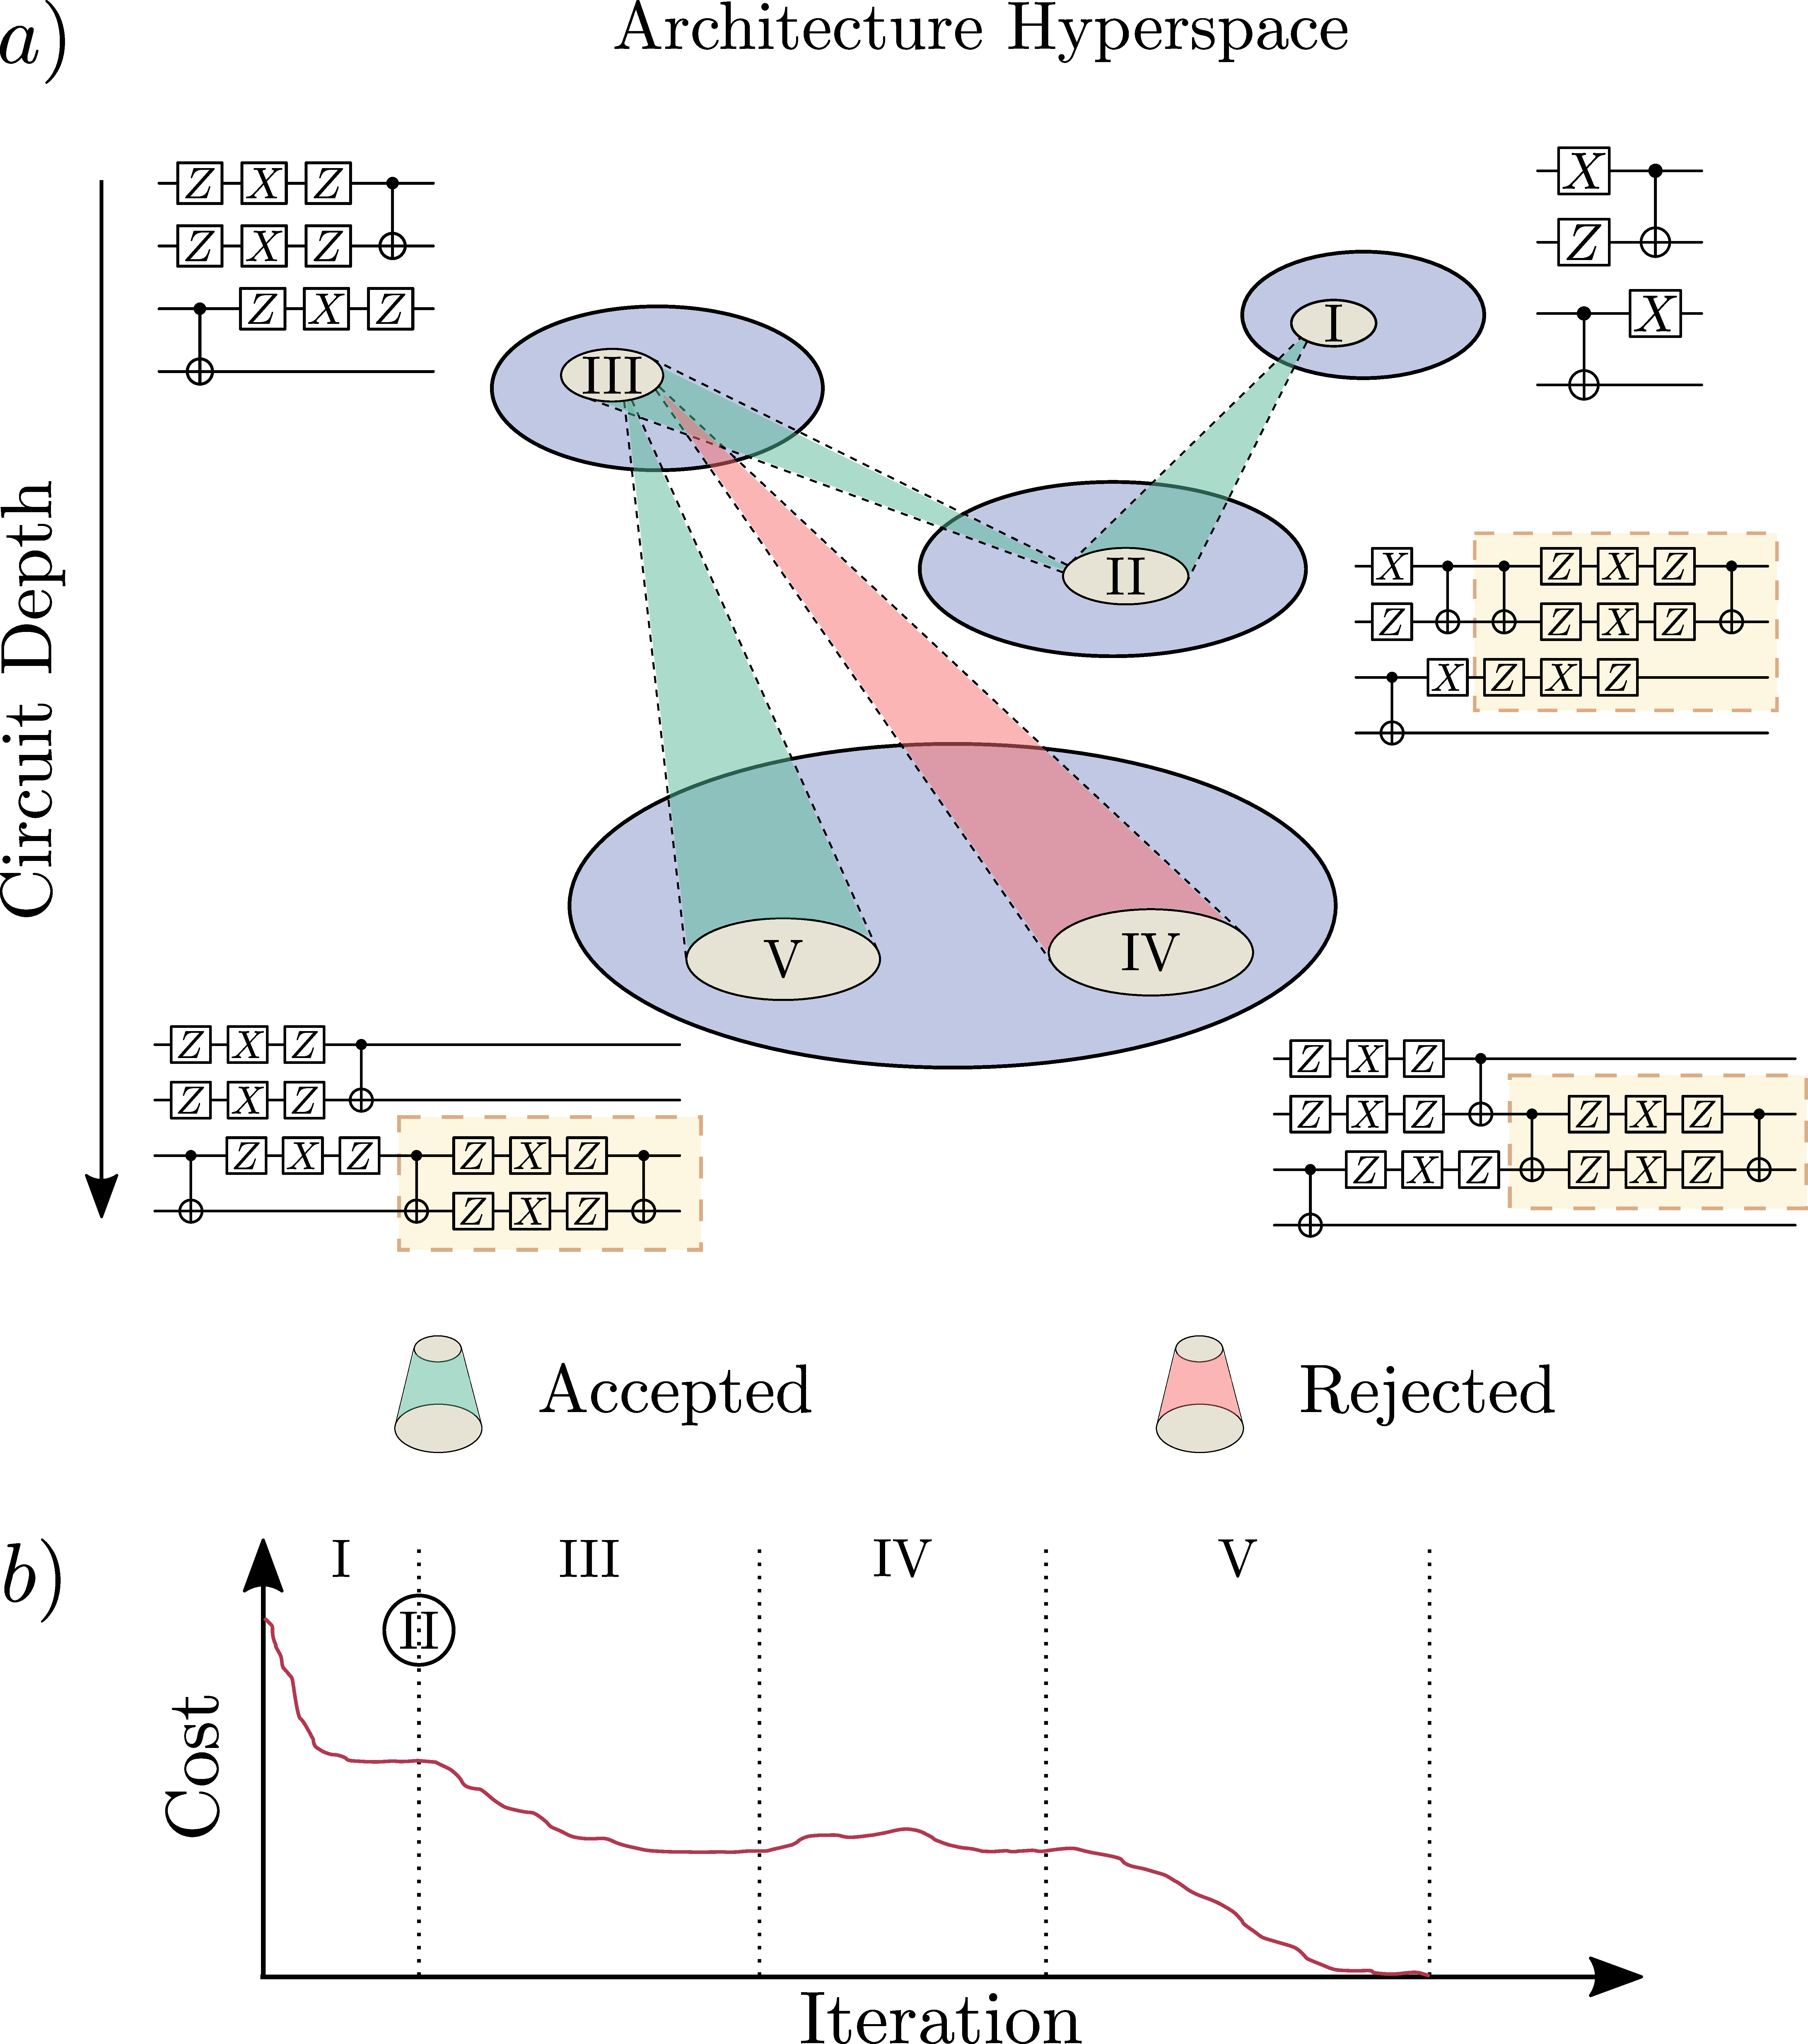
\includegraphics[width=.8\textwidth]{Figures/VANS/Fig1.pdf}
\caption{{\small We show a schematic diagram of the VAns algorithm. \textit{(a)} VAns explores the hyperspace of architectures of parametrized quantum circuits to create short depth ansatzes for VQA applications. VAns takes a (potentially non-trivial) initial circuit (step I) and optimizes its continuous parameters $\thv$ until convergence. At each step, VAns inserts blocks of gates into the circuit which are initialized to the identity (indicated in a box in the figure), so that the ansatzes at contiguous steps belong to an equivalence class of circuits leading to the same cost value (step II). VAns then employs a classical algorithm to simplify the circuit by eliminating gates and finding the shortest circuit (step II to III). The ovals represent subspaces of the architecture hyperspace connected through VAns. While some regions may be smoothly connected by placing identity resolutions, VAns can also explore regions that are not smoothly connected via a gate-simplification process. VAns can either reject (step IV) or accept (step V) modifications in the circuit structure. Here $Z$ ($X$) indicates a rotation about the $z$ ($x$) axis. \textit{(b)} Schematic representation of the cost function value versus the number of iterations for a typical VAns implementation which follows the steps in \textit{(a)}.}}
\label{fig:schematic}
\end{figure}

\afterpage{\clearpage}

To this end, we combine several features of recently proposed methods and introduce the Variable Ansatz (VAns) algorithm~\cite{bilkis2021semi} to generate variable structure ansatzes for generic VQA applications. As shown in Fig.~\ref{fig:schematic}, VAns iteratively grows the parameterized quantum circuit by adding blocks of gates initialized to the identity, but also prevents the circuit from over-growing by removing gates and compressing the circuit at each iteration. In this sense, VAns produces shallow circuits that are more resilient to noise, and that have less trainable parameters to avoid trainability issues. Our approach provides a simple yet effective way to address the ansatz design problem, without resorting to resource-expensive computations similar to recently evolutionary-oriented proposals.

Our algorithm is inspired by the strong presence of noise in NISQ devices. As such, it potentially hinders any successful application of NISQ computers. In this context, we should take advantage of every component of the quantum device that could be optimized over, and this generally includes the circuit's layout. In this regard, some approaches ---as EVQE~\cite{rattew2019domain} or MoG-VQE~\cite{chivilikhin2020mog} ---have been introdued in the past, as discussed in Sec.~\ref{ssec:1_nisq_vans_bp}. VAns algorithm differs from them in at least two important aspects: \textit{(i)} it considers general cost functions, and thus can be considered a general-purposed quantum-machine learning algorithm, and \textit{(ii)} the method incorporates knowledge on quantum computing via specific circuit compression rules.

Thus, the learning problem we are dealing with consists in finding cost-minimizing quantum circuits, where not only the parameters can be optimized, but also the structure of the circuit itself. While some light is shed into the learning problem through the aforementioned compression rules, an important \textit{learning-in-the-darkness} component remains. In particular, no structure is imposed on how our algorithm grows the quantum circuit, and at each time-step quantum gates are randomly placed across the circuit, acting on qubits that are also randomly selected. Thus, the learning paradigm departs from the one considered in Chapter~\ref{chapter:RLCOH}, and rather than assuming complete ignorance of the setting, the agent (VAns algorithm) is now equipped with partial information about the setting, henceforth it learns in the twilight through the VAns algorithm, which we now turn to explain in detail.

\subsection{Gaussian systems}\label{ssec:intro_cv_gaussianinfo}
We define Gaussian quantum states as thermal states of a quadratic hamiltonians
\eq{rhog}{\rho_G = \frac{e^{-\beta \hat{H}}}{\tr{e^{-\beta \hat{H}}}} \space,   \; \; \beta\in\mathbb{R}^+,}
\eq{hamiGauss}{\hat{H} = \frac{\rop^T H \rop}{2} + \rop^T \rvec,}
where $\rvec$ is a constant vector in phase space, and $H$ is the \textit{Hamiltonian matrix}, which is positive-defined and symmetric. Note this definition includes the limit $\beta \rightarrow \infty$, which corresponds to the case of pure states.

Such construction allows us to find the so-called normal mode form of $\rho_G$, in which the system behaves as a set of $n$ decoupled harmonic oscillators. In particular, studying the transformation that takes $\rho_G$ into its normal form is instructive, and we will comment on it nextly. %when studying the structure of gaussian states.
%
% Let us understand the structure of $\hat{H}$ in detail.
There are at least two important reasons to study Gaussian states. Firstly, many problems become analytically tractable when dealing with such a class. Secondly, manipulating Gaussian states is experimentally feasible. Moreover, light (\textit{e.g}) is a natural candidate for quantum communication scenarios, and coherent states --- a particular type of Gaussian states --- describe very well the behaviour of lasers.

We note that, up to a constant shift in the energy landscape, $\hat{H}$ is equivalent to
\eq{h1}{\hat{H}' = \frac{(\rop - \rbar)^T H (\rop - \rbar)}{2},  \spacee \rbar = - H^{-1} \rvec.}
Note that $H^{-1}$ does always exists since $H>0$. It follows that
\eq{hp}{\hat{H}' = \frac{1}{2} \weyl{-\rbar} \rop^T H \rop \weyl{\rbar},}
we can thus focus on the non-displaced hamiltonian $\rop^T H \rop$. In the Heisenberg picture, the evolution of canonical operators corresponds to $\dot{\rop}_j = \ii \Comm{\hat{H}}{\rop_j}$, and by using the CCR, it follows that $\dot{\rop} = \Omega H \rop$. Thus, we conclude that $\rop(t) = e^{\Omega H t} \rop(0)$.
Since any system transformation should preserve the CCR, it follows that
\eq{pres}{\ii \Omega = \Comm{\rop(t)}{\rop^T(t)} =  e^{\Omega H } \Comm{\rop(0)}{\rop(0)^T} (e^{\Omega H })^T  = \ii e^{\Omega H } \Omega (e^{\Omega H })^T,}
and thus
\eq{symp}{\Omega = S \Omega S^T, \spacee S:= e^{\Omega H t}.}
The last line is the condition for $S$ to belong to the real symplectic group $\symp$, which is the reason for calling $\Omega$ the symplectic form. If we now explicit the unitary character of canonical operators' time-evolution, we obtain
\eq{00}{\dot{\rop} = \hat{U}^\dagger(t) \rop(0) \hat{U}(t) = e^{- \ii \hat{H} t} \rop(0) e^{\ii \hat{H} t} = e^{\Omega H t} \rop(0) = S \rop(0),}
we see that there is a clear correspondence between unitary operators and symplectic transformations, and in fact $\symp \cap SO(2n)$ is a isomorphic to $U(n)$. Thus, there is a correspondence between symplectic transformations $S=e^{\Omega H}$ and unitary operators generated by second-order hamiltonians, $\sh=e^{\frac{\ii \rop^T H \rop}{2}}$:
\eq{sympo}{\sh \rop \sh^\dagger = S \rop.}
In particular, said symplectic transformation $S$ can be written in its singular value decomposition as
\eq{svdS}{S = O_1 Z O_2,}
where $O_1, O_2 \in \symp\cap SO(2n)$ are orthogonal symplectic transformations and $Z = \bigoplus_{j=1}^{n}\begin{pmatrix}z_j&0\\0&z_j^{-1}\end{pmatrix}$ stands for the \textit{squeezing} transformation. The energy of the system ($\rop^T\rop$) is invariant under the action of $O_i$, and thus we refer to those transformations as \textit{passive} ones. Importantly, the isomorphism with the unitary group guarantees that such symplectic transformations can be constructed out from \textit{phase-shifters} and \textit{beam-splitters}~\cite{Reck1994Experimental,Weedbrook2012Gaussian}.

In particular, phase-shifters $R_\phi$ and beam-splitters $B_{\theta,\psi}$
have the following matrix representations
\eq{passive1}{R_\phi = \begin{pmatrix}\cos\phi&\sin\phi\\ -\sin\phi & \cos\phi\\ \end{pmatrix},\spacee B_{\theta,\psi}=\begin{pmatrix}\cos\theta&e^{i\psi}\sin\theta\\ -e^{-\ii \psi}\sin\theta& \cos\theta\\ \end{pmatrix}\otimes \mathbb{I}_2.}
In passing, we note that if we move the anhilation and creation operators, the action of phase-shifters is that of adding a phase $e^{\ii \phi}$, whereas beam-splitters mix two modes $a_1$ and $a_2$ (which correspond to the input modes):
\begin{align}\label{eq:colhonbs}
B_{\theta,\psi}^\dagger \hat{a}_1 B_{\theta,\psi} &= \cos\theta \hat{a}_1 + e^{\ii\psi}\sin\theta \hat{a}_2 \\
B_{\theta,\psi}^\dagger \hat{a}_2 B_{\theta,\psi} &=  -e^{-\ii\psi}\sin\theta \hat{a}_2 +\cos\theta \hat{a}_1,
\end{align}
where the added phase $\psi$ can, for instance, be corrected via a proper phase-shift.

To sum up, any simplectic transformation can be implemented out of squeezing operations and interferometers (\textit{e.g.} a combination of phase-shifters and beam-splitters, which can in turn mimic any passive simplectic transformation.%~\cite{Reck1994Experimental}).

Let us now focus on the structure of the Hamiltonian matrix $H$. In particular, we recall that given $M\in\mathbb{R}^{2n\times2n}$, with $M>0$, there exists a transformation $S\in\symp$ taking $M$ into its normal form~\cite{Williamson1936Algebraic}, \textit{e.g.} $SMS^T = D$  with $D = \bigoplus_j d_j\mathbb{I}_2$ %\text{diag}\big(d_1,d_1...d_n,d_n\big)
containing the symplectic eigenvalues $\llaves{d_j}_{j=1}^n$; recall that such transformation can be challenging to find~\cite{pereira2021symplectic, Pirandola2009correlation}. In this regard, $S$ is related to the transformation
$L$ that puts $\ii \Omega M$ into its diagonal form, \textit{e.g.}
$L \Omega M L^{-1}$ is diagonal, with $S = (L^{-1} \bar{U})^\dagger$, and the symplectic eigenvalues of $M$ are the (absolute values of) the eigenvalues of $\ii \Omega M$, which come into pairs $\llaves{\pm d_j}_{j=1}^n$.
We can readily apply such decomposition to our quadratic Hamiltonian matrix $H$:
\equ{H = S^T \big( \bigoplus_{j=1}^n \omega_j \id_2 \big) S,}
where by denoting the symplectic eigenvalues by $\omega_j$ we highlight its role as frequencies of $n$ non-interacting free modes.
By inserting such normal mode decomposition into $\hat{H}$:
\begin{align}
\hat{H} &= \frac{1}{2} \rop^T H \rop \\
&= \frac{1}{2} \rop^T S^T \big(\bigoplus_{j=1}^n \omega_j \id^{(j)}_2 \big)S \rop
\end{align}
We now use that the symplectic transformation $S$ has a unitary representation $\sh$:
\begin{align}
\hat{H} &= \frac{1}{2} \rop^\dagger H \rop \\
&= \frac{1}{2} \hat{S} \rop^T \big(\bigoplus_{j=1}^n \omega_j \id^{(j)}_2 \big) \rop \hat{S}^\dagger
\end{align}
Upon defining $\hoj := \frac{\omega_j}{2}(q_j^2 + p_j^2)$, we note that any second-order Hamiltonian with zero displacement is equivalent (up to a unitary transformation) to a set of decoupled oscillators. The decomposition of the original quadratic hamiltonian reads
\begin{align}
\hat{H} &= \frac{1}{2} (\rop - \rbar)^T H (\rop - \rbar) \\
&= \weyl{-\rbar} \hat{S} \big( \sum_{j=1}^n \hoj\big) \hat{S}^\dagger \weyl{\rbar},
\end{align}
which implies that gaussian states have the following structure:
\begin{align}\label{eq:1gaussrho}
\rho_G &= \frac{\weyl{-\rbar} \hat{S} \big( \bigotimes_{j=1}^n e^{- \beta \hoj} \big) \hat{S}^\dagger \weyl{\rbar} }{ \prod_j\tr{e^{-\beta \hoj} }} \\
&= \mathcal{N}_\beta \weyl{-\rbar} \hat{S}^\dagger \big( \bigotimes_{j=1}^n \sum_{k_j=0}^\infty e^{- \beta k_j \omega_j} \proj{k_j} \big) \hat{S} \weyl{\rbar},
\end{align}
where in the second line we have expanded $\hoj$ in the Fock basis $\llaves{\proj{k_j}}$ of each mode $j$, and defined $\mathcal{N}_\beta  := \prod_j (1-e^{-\beta \omega_j})$. We observe that for $\beta \rightarrow \infty$ a pure state is obtained, since only vacuum terms survive. Hence, pure gaussian states are generated by applying gaussian unitary operations to the n-mode vacuum state. Quite remarkably, either Gaussian states have rank 1 (pure states), or infinite rank (mixed states).

We thus conclude that Gaussian states are obtained from orthogonal symplectic transformations (and displacements) applied to a set of non-interacting harmonic oscillators. In particular, the action of such transformations is lineal in phase space, a fact that becomes clear when inspecting its action on the statistical moments.

\subsection{Some methods in phase space}\label{ssec:intro_cv_phase}
Another parametrization of Gaussian states can be obtained, by departing from Eq.~\ref{eq:1gaussrho}; in particular we note that the first two moments of $\rho_G$ encode all its information, as
\begin{align}\label{eq:1moms}
 \rbar&:=\tr{\rho_G \rop}   \\
\cov&:= \tr{ \llaves{\rop - \rbar, (\rop - \rbar)^\dagger} \rho} = S \big(\bigoplus_j \nu_j \id_2^{(j)} \big)S^T,\nonumber
\end{align}
where $\nu_j = \dfrac{1+e^{-\beta \omega_j}}{1-e^{-\beta \omega_j}} $ stand for the symplectic eigenvalues of $\cov$\footnote{Note that for the single-mode case, the covariance reads $\cov_{nm} = \expect{\Delta \rop_n \Delta \rop_m} + \expect{\Delta \rop_m \Delta \rop_n}$, with $\Delta \rop_i = \rop_i - \expect{\rop_i}$, and $\rop = (q, p)$.}.
All the information about the Gaussian state is encoded in both the expectation value and covariance. On the one hand, the displacement value $\bm{\bar{r}}$ stand for the first statistical moment of the Gaussian state. On the other hand, the symplectic transformation $S$ (associated to the gaussian unitary $\sh$), as well as the symplectic eigenvalues of $H$ can be obtained through $\cov$. In this regard, we note that the spectrum of the Guassian state can be obtained from the covariance matrix, and thus correlation measures between the modes, as well as the states' purities, can be inferred from the second statistical moment.

%%% robertson- schrodinger
Importantly, any covariance matrix $\cov$ of a quantum state should satisfy the Robertson-Schrödinger uncertainty relation
\eq{uncer}{\cov + \ii \Omega \geq 0,}
which is a direct consequence of the CCR and the positivity of the quantum state $\rho$.
The singular value decomposition of symplectic transformations in~\eqref{eq:svdS} turns useful to understand the structure of the covariance matrix. For example, if we restrict to pure Gaussian states, then it follows that
\begin{align}\label{eq:pure_cov_gauss}
\cov = O D O^T,
\end{align}%single-mode Gaussian states, it follows that $\cov = \nu O D O^T$, with $D=\text{diag}(d, \frac{1}{d})$, whereas if we consider $n$can be inserted into the expression
where $D = \bigoplus_{j=1}^n\begin{pmatrix}d_j&0\\0&\frac{1}{d_j}\\\end{pmatrix}, \; d_j>0$ and $O$ stands for a passive, orthogonal transformation. Moreover, if we restrict to single-mode systems, we observe that covariance matrices are generated by squeezing and rotating the identity; this is aligned with the fact that all pure gaussian states can be obtained through symplectic tranformations applied to the vacuum state $\ket{0}^{\otimes n}$.

While preparation of pure Gaussian states has such intuitive interpretation, this picture can be complemented with a collection of quasiprobability distributions that depict the quantum state in phase space which we now turn to present.

In analogy to classical mechanics, we can study the quantum system in phase space. In doing so, we arrive to the so-called quasiprobability density functions, which are equivalent to the quantum state and provides yet another operational approach to its characterisation. Unsurprisingly, such analogy finds frontiers, since such quasiprobability distributions can take negative values (for instance, for non-Gaussian states). In this regard, we find that the set of quantum Gaussian states behave classically, since their associated quasiprobabilities are --- spoiler alert --- Gaussian distributions.

The phase-space formalism hinges on the overcompleteness of Weyl operators, which serves as a bridge between Hilbert and phase spaces. In the following we will restrict to the \textit{single}-mode case; generalizations to $n$-mode systems are straightforward.

Recall that a coherent state is defined an eigenstate of $\hat{a}$
\eq{def_coherent}{\begin{cases} \hat{a} \weyl{\alpha} \ket{0} = \alpha \weyl{\alpha}\ket{0} \\ \ket{\alpha} = \weyl{\alpha} \ket{0} \end{cases}.}
In particular, note that $\proj{\alpha} = \weyl{\alpha}\proj{0}\weyl{\alpha}^\dagger$, meaning that coherent states are --- in line with the formalism revisted in the provious section --- just displaced vacuum states, with idle symplectic transformations and thus an identity as covariance matrix. In particular, by writing such states in the Fock basis, we obtain
\eq{1fockcoherent}{\ket{\alpha} = e^{-\frac{|\alpha|^2}{2}} \sum_{n=0}^\infty \frac{\alpha^n}{\sqrt{n}}\ket{n},}from which it is not hard to prove that coherent states resolve to identity:
\eq{resocoh}{\frac{\int_\mathbb{C} \proj{\alpha} d^2\alpha}{\pi} = \id.}
This shows that coherent states resolve to a measurement, called \textit{heterodyne} measurement. Moreover, given any (bounded) operator $\hat{O}$, we can express it as
\begin{align}\label{eq:trW}
\hat{O} &= \frac{1}{\pi} \int_{\mathbb{C}}d^2\alpha \tr{\hat{O} \weyl{\alpha} }\weyl{-\alpha},\\
\tr{\hat{O}} &= \frac{1}{\pi}\int_\mathbb{C} d^2\alpha \langle\alpha|\hat{O}|\alpha\rangle,
\end{align}
which is known as the \textit{Fourier-Weyl relation}. This allows us to write any quantum state $\rho$ in terms of coherent states as
\equ{\rho = \frac{1}{\pi} \int_{\mathbb{C}} \tr{ \rho \weyl{\alpha}} \weyl{-\alpha}.} In particular, the \textit{characteristic function} $\chi(\alpha)$ is defined as the coefficient accompaying $\weyl{-\alpha}$ in the integral, \text{e.g.}
\begin{align}
\chi(\alpha) &= \tr{ \rho \weyl{\alpha}}\\
\rho &= \frac{1}{\pi} \int_{\mathbb{C}} \chi(\alpha)\weyl{-\alpha}.
\end{align}
Such characteristic function allows us to define% quasiprobability distributions, according to
% \eq{qpd}{W_s(\alpha) = \frac{1}{\pi^2} \int_{\mathbb{C}} d^2 \beta \chi_s(\beta) e^{\alpha \bar{\beta} - \bar{\alpha} \beta}}, where it can be checked that $\int W_s(\alpha) d^2 \alpha = 1$.
% Moreover,
the Wigner function as its (complex) Fourier transform:
\eq{qpd}{W(\alpha) = \frac{1}{\pi^2} \int_{\mathbb{C}} d^2 \beta \chi(\beta) e^{\alpha \bar{\beta} - \bar{\alpha} \beta},}
which satisfies that $\int W(\alpha) d^2 \alpha = 1$. By expanding $\alpha = \frac{q + \ii p}{\sqrt{2}} $ and $ \beta = \frac{\tilde{q} + \ii \tilde{p}}{\sqrt{2}}$, we find that $W(q,p) = \int d\tilde{q} e^{\ii p \tilde{q}} \langle q + \tilde{q}| \rho | q - \tilde{q}\rangle$.
Such parametrization provides an operational interpretation of Wigner functions, since $\frac{1}{2}\int_\infty^\infty dp W(q,p)= \langle q |\rho |q\rangle$, \textit{e.g.} marginal distributions predict probability measurement outcomes over conjugate variables and if varying the direction of $p$ in the integrand one can perform a tomographic reconstruction of the quantum state.
\begin{figure}[t!]
\centering
    \begin{subfigure}[b]{0.49\textwidth}
        \centering
        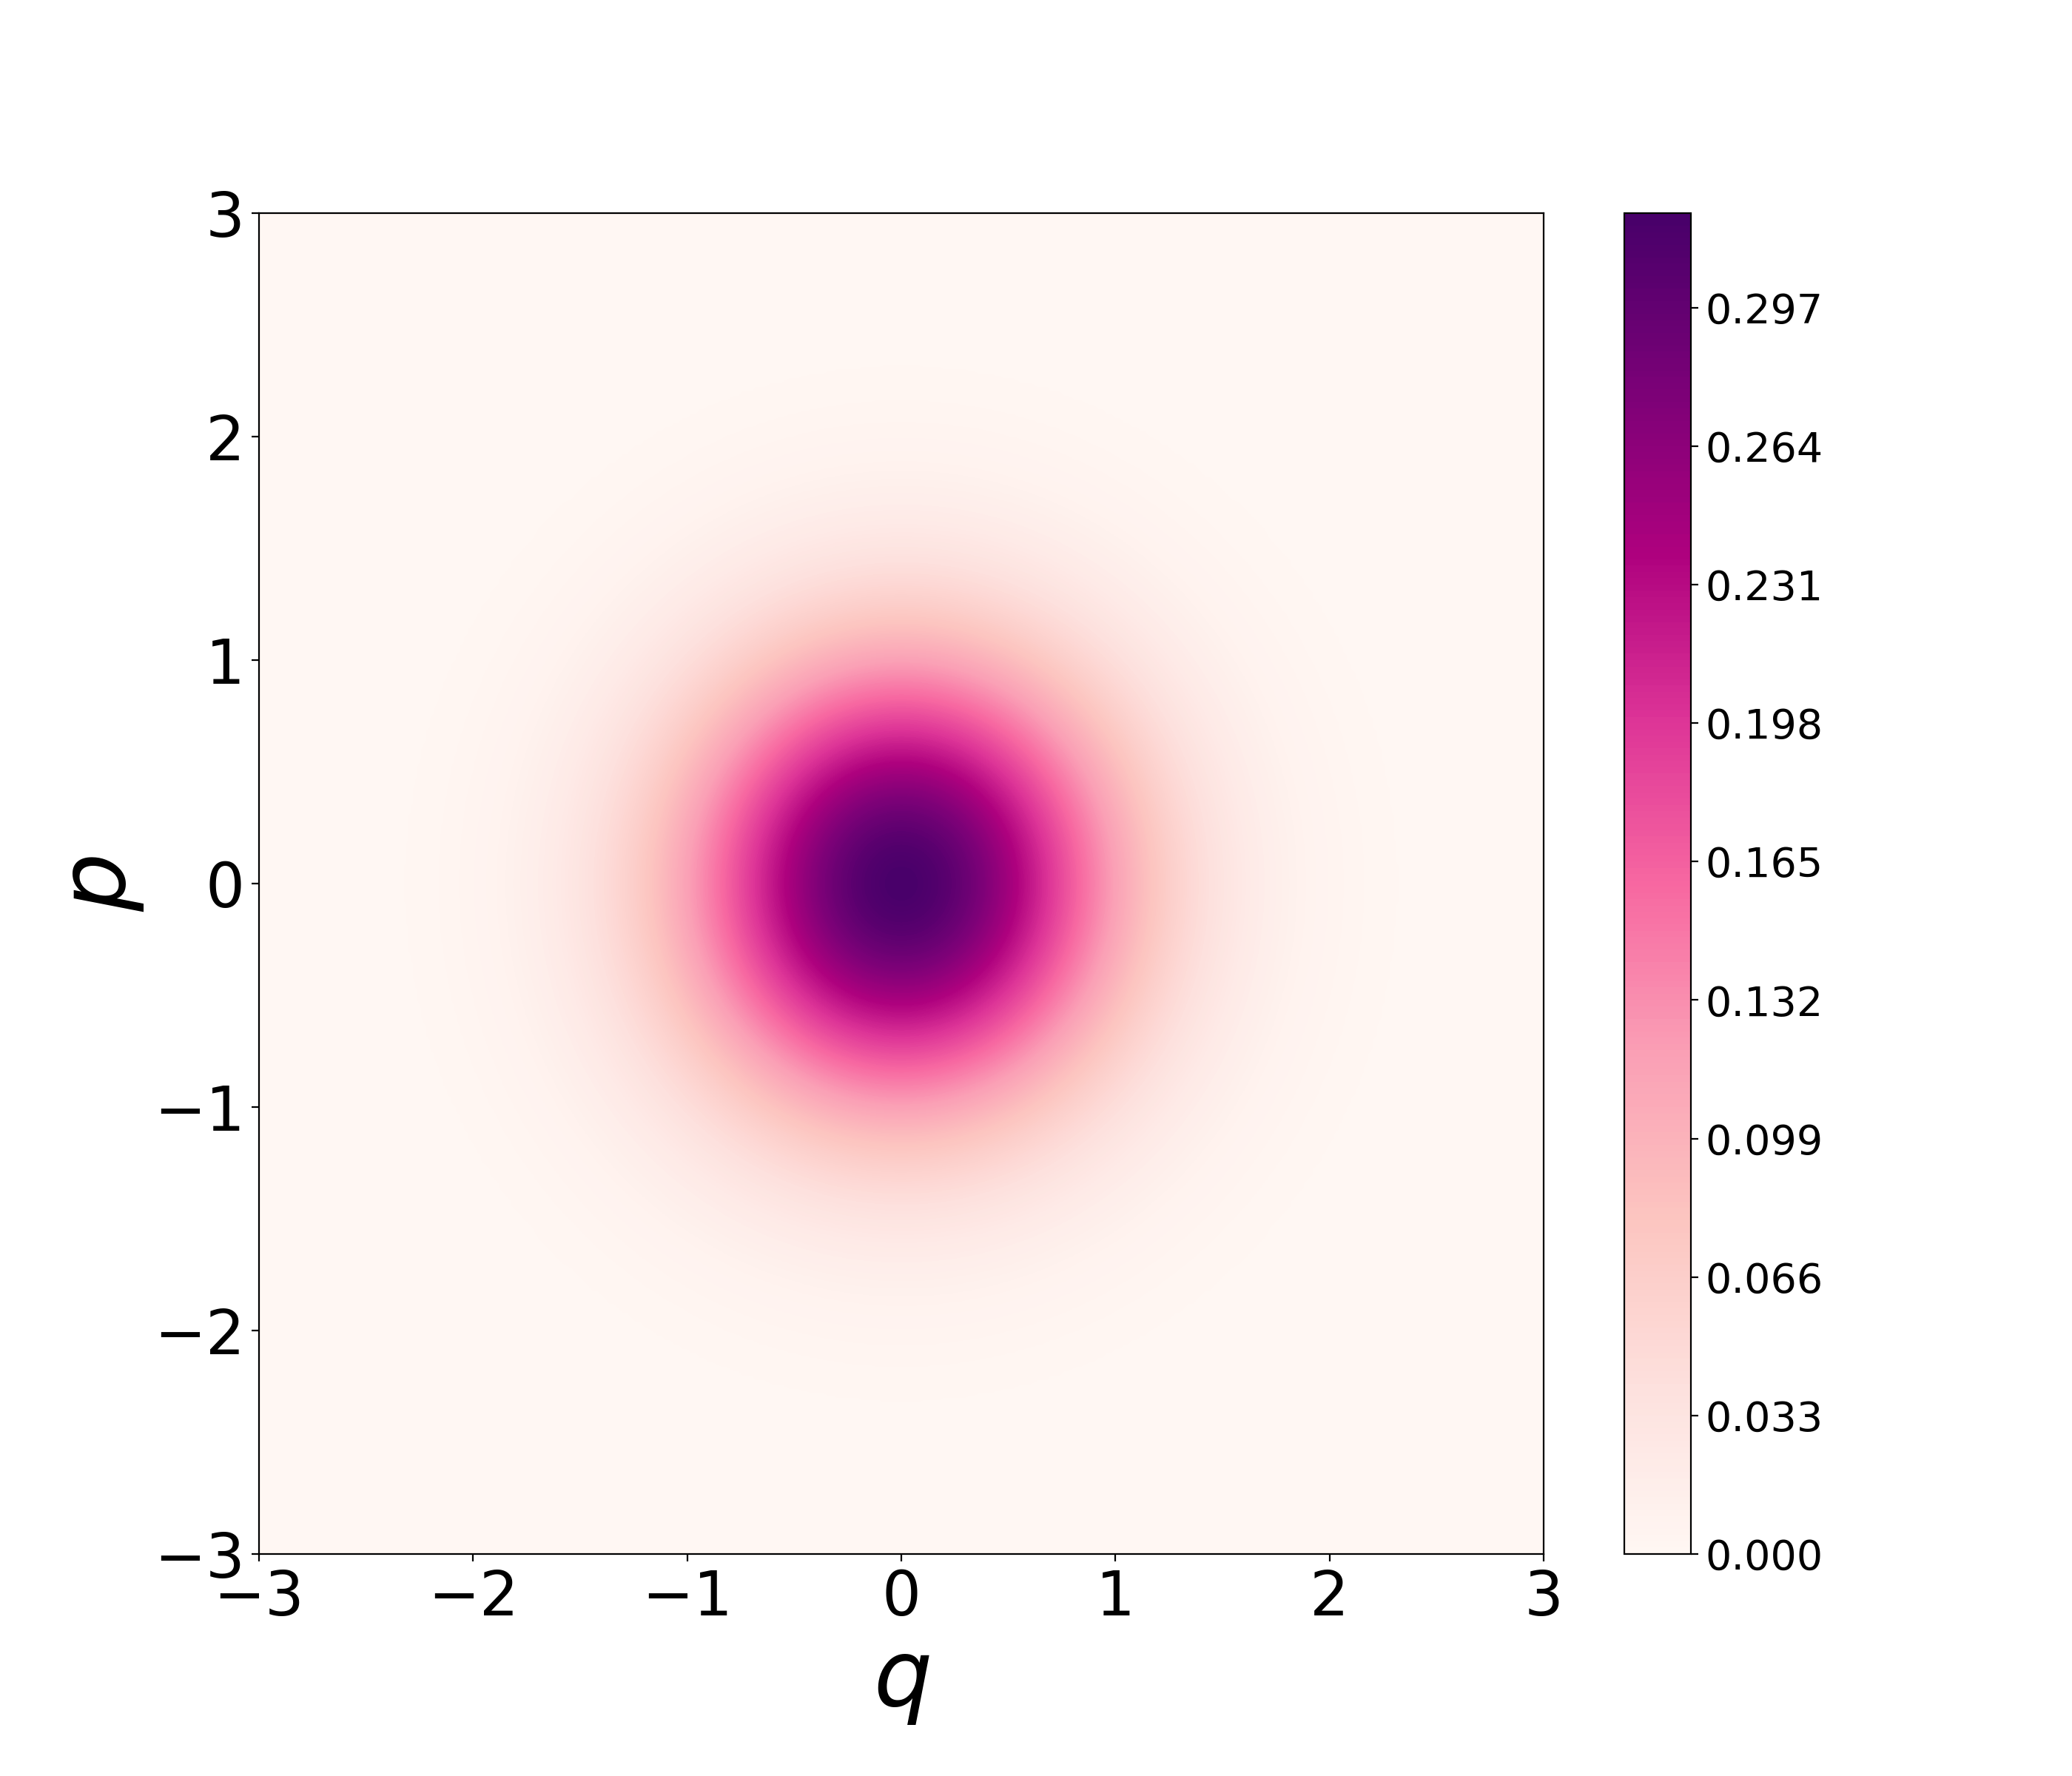
\includegraphics[width=1.\textwidth]{Figures/some_wigners/vacuum.png}
    \end{subfigure}
    \hfill
    \begin{subfigure}[b]{0.49\textwidth}
        \centering
        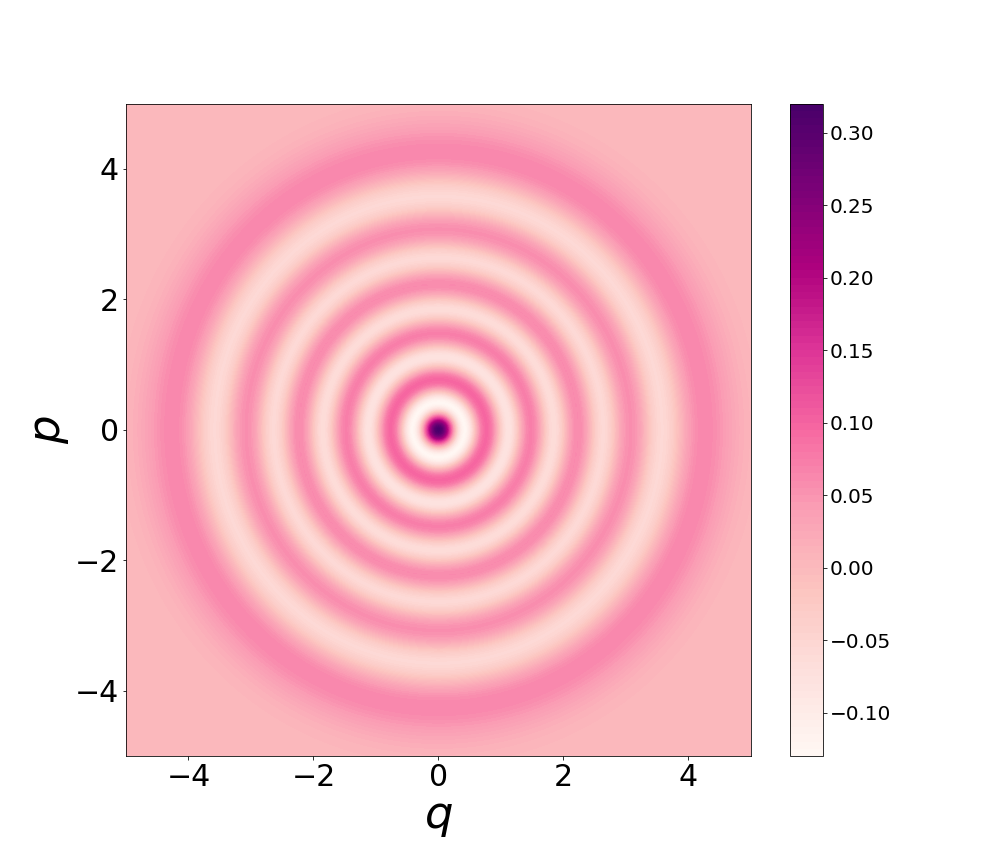
\includegraphics[width=1.\textwidth]{Figures/some_wigners/fock5.png}
    \end{subfigure}
\caption{We show the Wigner functions of the vacuum state $\ket{0}$ (left) and of the Fock state $\ket{5}$ (right). While in the former case the probability distribution is a Gaussian, the latter represents a non-Gaussian state (\textit{e.g.} is the fifth eigenstate of the harmonic oscillator), which here translates into negative values of the Wigner function. }
\label{fig:wigners}
\end{figure}
Finally, for Gaussian states, the characteristic and Wigner functions are Gaussians, \textit{e.g.}
\begin{align}\label{gauss_char_wigner}
\chi(\rvec) &= e^{-\frac{(\Omega \rvec)^T\cov \Omega \rvec}{2} - \ii (\Omega \rvec)^T \bar{\bm{r}}} \\
W(\rvec) &= \frac{2^n}{\pi^n \sqrt{|\cov|}}e^{-(\rvec - \bar{\bm{r}})^T\cov^{-1}(\rvec - \bar{\bm{r}})}.
\end{align}
In Fig.~\ref{fig:wigners} we show two examples of such Wigner functions, one for a coherent (and thus Gaussian) state, and other one for a Fock number state; we observe in the latter case that the Wigner function can take negative values: such negativity play a role of a classical-quantum frontier in continuous-variable systems~\cite{nongaussian}.

We have thus identified the set of Gaussian states as thermal (and ground) states of quadratic hamiltonians. Equivalently, Gaussian states can be defined as those whose characteristic function is Gaussian. On the one hand, we have observed that Gaussian states can be understood as a set of $n$ non-interacting harmonic oscillators, up to a symplectic transformation $\sh$. Such symplectic transformation is ultimately linked to a Gaussian unitary, \textit{e.g.} generated by a quadratic hamiltonian. Moreover, Eq.~\ref{eq:1moms} explicits the action of such transformations on the first two statisitcal moments of the Gaussian state, namely displacing the canonical coordinates and transforming the covariance matrix via a simplectic matrix that acts by similarity. In turn, such operations act linearly in phase space and that is the reason for which Gaussian operations are deemed so in literature~\cite{Weedbrook2012Gaussian,Olivares2012}.

\subsection{Gaussian operations and beyond}\label{ssec:1_cv_channels}
% While Gaussian unitary transformations act as either displacing, rotating or squeezing gaussian distributions in phase space, we might explicit a more expedient characterization of Gaussian transformations.
A quantum channel is deemed Gaussian if it preserves the Gaussian character of the state. Such definition applies to unitary transformations, but also to CP-maps (which can suitably be obtained via a Stinespring dilation with an ancilla).% Moreover, such definition also holds for quantum measurements, in such case the outcome distribution is required to be Gaussian whenever the measured state is Gaussian as well.


A handful parametrization of Gaussian CP-maps can readily be obtained by studying the evolution of system's state after a Gaussian unitary interaction with a (Gaussian) auxiliary system. The result is an update rule for the first two moments, parametrized by matrices $X$ and $Y$ in $\mathbb{R}^{2n\times2n}$:
\begin{align}\label{eq:1_cv_gaussianCPmap}
\bm{\bar{r}} &\rightarrow X \bm{\bar{r}}\\
\cov &\rightarrow X \cov X^T + Y,
\end{align}
with $Y + \ii \Omega \geq \ii X\Omega X^T$ (such condition guarantees that Robertson-Schrödinger uncertainty relations in Eq.~\eqref{eq:uncer} are preserved). We note that such evolution is different than the resulting one when continuously monitoring the system, as studied in Sec.~\ref{sec:1_cmon}.

In particular an attenuator --- or \textit{lossy} channel --- is obtained by mixing a quantum state with the vacuum by a beam-splitter, and we denote it by $\mathcal{L}_\eta$, where $\eta$ is the transmissivity coefficient. For such a channel, and restricting to the single-mode case, one finds that $X=\eta \mathbb{I}_2$ and $Y = \sqrt{1-\eta^2}\mathbb{I}_2$, with $\eta\in[0,1]$. We note that if the input state is a coherent state, the covariance matrix remains unchanged (since $\cov = \mathbb{I}_2$), whereas the first moment gets attenuated as $\alpha \rightarrow \eta \alpha$. This channel turns to accurately model the behaviour of a laser beam transmitted through the atmosphere, though the transmissivity $\eta$ non-trivially depends on parameters such as height, temperature and
 more~\cite{Dequal2020,Andrews2005,Usenko2012a,Pirandola2021,Pirandola2021a,Vasylyev2011,Vasylyev2017}.

\subsection{Measurements}\label{ssec:1_cv_measurements}
A measurement is deemed gaussian if \textit{(i)} it preserves the Gaussian character of the state upon post-conditioning, and \textit{(ii)} when measuring a Gaussian state, the outcome probability distribution is Gaussian.
For instance, counting excitations correspond to projections over Fock states: recall that $\sum_{n=0}^\infty \proj{n} = \mathbb{I}$), and are obviously non-gaussian since number states (asside from vacuum) are not; moreover, the underlying distribution is Poissonian. Nevertheless, it is experimentally possible (though expensive) to resolve excitations in quantum optics laboratories, thorugh an apparatus known as \textit{photon-counter}~\cite{Photoncounter}. In this regard, one may be interested in only resolving between ```no photons'' or ```one or more photons'', an apparatus known as \textit{on/off photodetector}, which correspond to jut partitioning the Hilbert space differently, \textit{e.g.} $\mathcal{M}_{on/off} = \llaves{\proj{0}, \mathbb{I}-\proj{0}}$, where the second measurement operator is non-gaussian.

Le us know restrict to Gaussian projections. In particular, we have mentioned homodyne detection corresponds to projecting over a quadrature direction in phase space, as defined by the operator $\hat{q}_\theta = \cos\theta \hat{q}+ \sin \theta \hat{p}$, where $\hat{q}_\theta \ket{q_\theta} = q_\theta \ket{q_\theta}$ and $\mathbb{I} = \int_\mathbb{R} \proj{q_\theta} dq_\theta$, and $p(q_\theta) = \tr{\proj{q_\theta} \rho}$.
Such measurement can be realized, for instance, by the so-called \textit{balanced} homodyne detection. This consists in mixing $\rho$ with a local oscillator ($\ket{\alpha}$ with $|\alpha|\gg1$) by a balanced beam-splitter ($\theta = \frac{\pi}{4}$ and $\psi=0$ in Eq~\ref{eq:colhonbs}), and substracting the detected intensities at the two outputs of the beam-splitter (each measured by a photodetector). An alternative way to realize a homodyne detection is the \textit{direct} homodyne detection, which consists on mixing the incoming signal with a local oscillator by a low-reflectivity BS (which transmits most of the original signal, adding only a small amount of the local oscillator) and measuring the intensity of the reflected port.

On the other hand, we can consider heterodyne measurements, which in accordance to Eq.~\eqref{eq:resocoh} are projective measurements on coherent state of varying intenstity and phase. They can be realized by combining the state $\rho$ with a vacuum into a balanced beam splitter, and homodying in the direction of $\hat{q}$ and $\hat{p}$ (\textit{e.g.} $\theta = 0 $ and $\theta = \frac{\pi}{2}$ in Eq.~\ref{eq:passive1} respectively) in the paragraph of above); in this regard heterodyne measurements correspond to joint measurements of position and momenta, and its probability measurement outcome is $p(\alpha) = \langle\alpha|\rho|\alpha\rangle\pi^{-1}$.

Such a mechanism of implementing a measurement by homodying and having access to ancillas can actually be generalized to any Gaussian operation via Gaussian ancillas, Gaussian unitary interactions and homodyning/discarding the reduced state of the ancilla system~\cite{Cirac2002Characterization}.

%

\section{Continuously-monitored systems}\label{sec:1_cmon}
Our focus in this Section will be put on continuously-monitored quantum systems. Opposite to the previously discussed single-shot scenarios, here we are interested in measuring the system repeatedly, which in the continuous limit leads to a \textit{measurement signal}. Here, we will give an introduction to the topic, and the interested reader is encouraged to complement our discussion with Refs.~\cite{wisemanbook,jacobs_2014,gardiner1985input, doherty1999feedback,wiseman1993interpretation}.

\begin{figure}[t!]
    \centering
    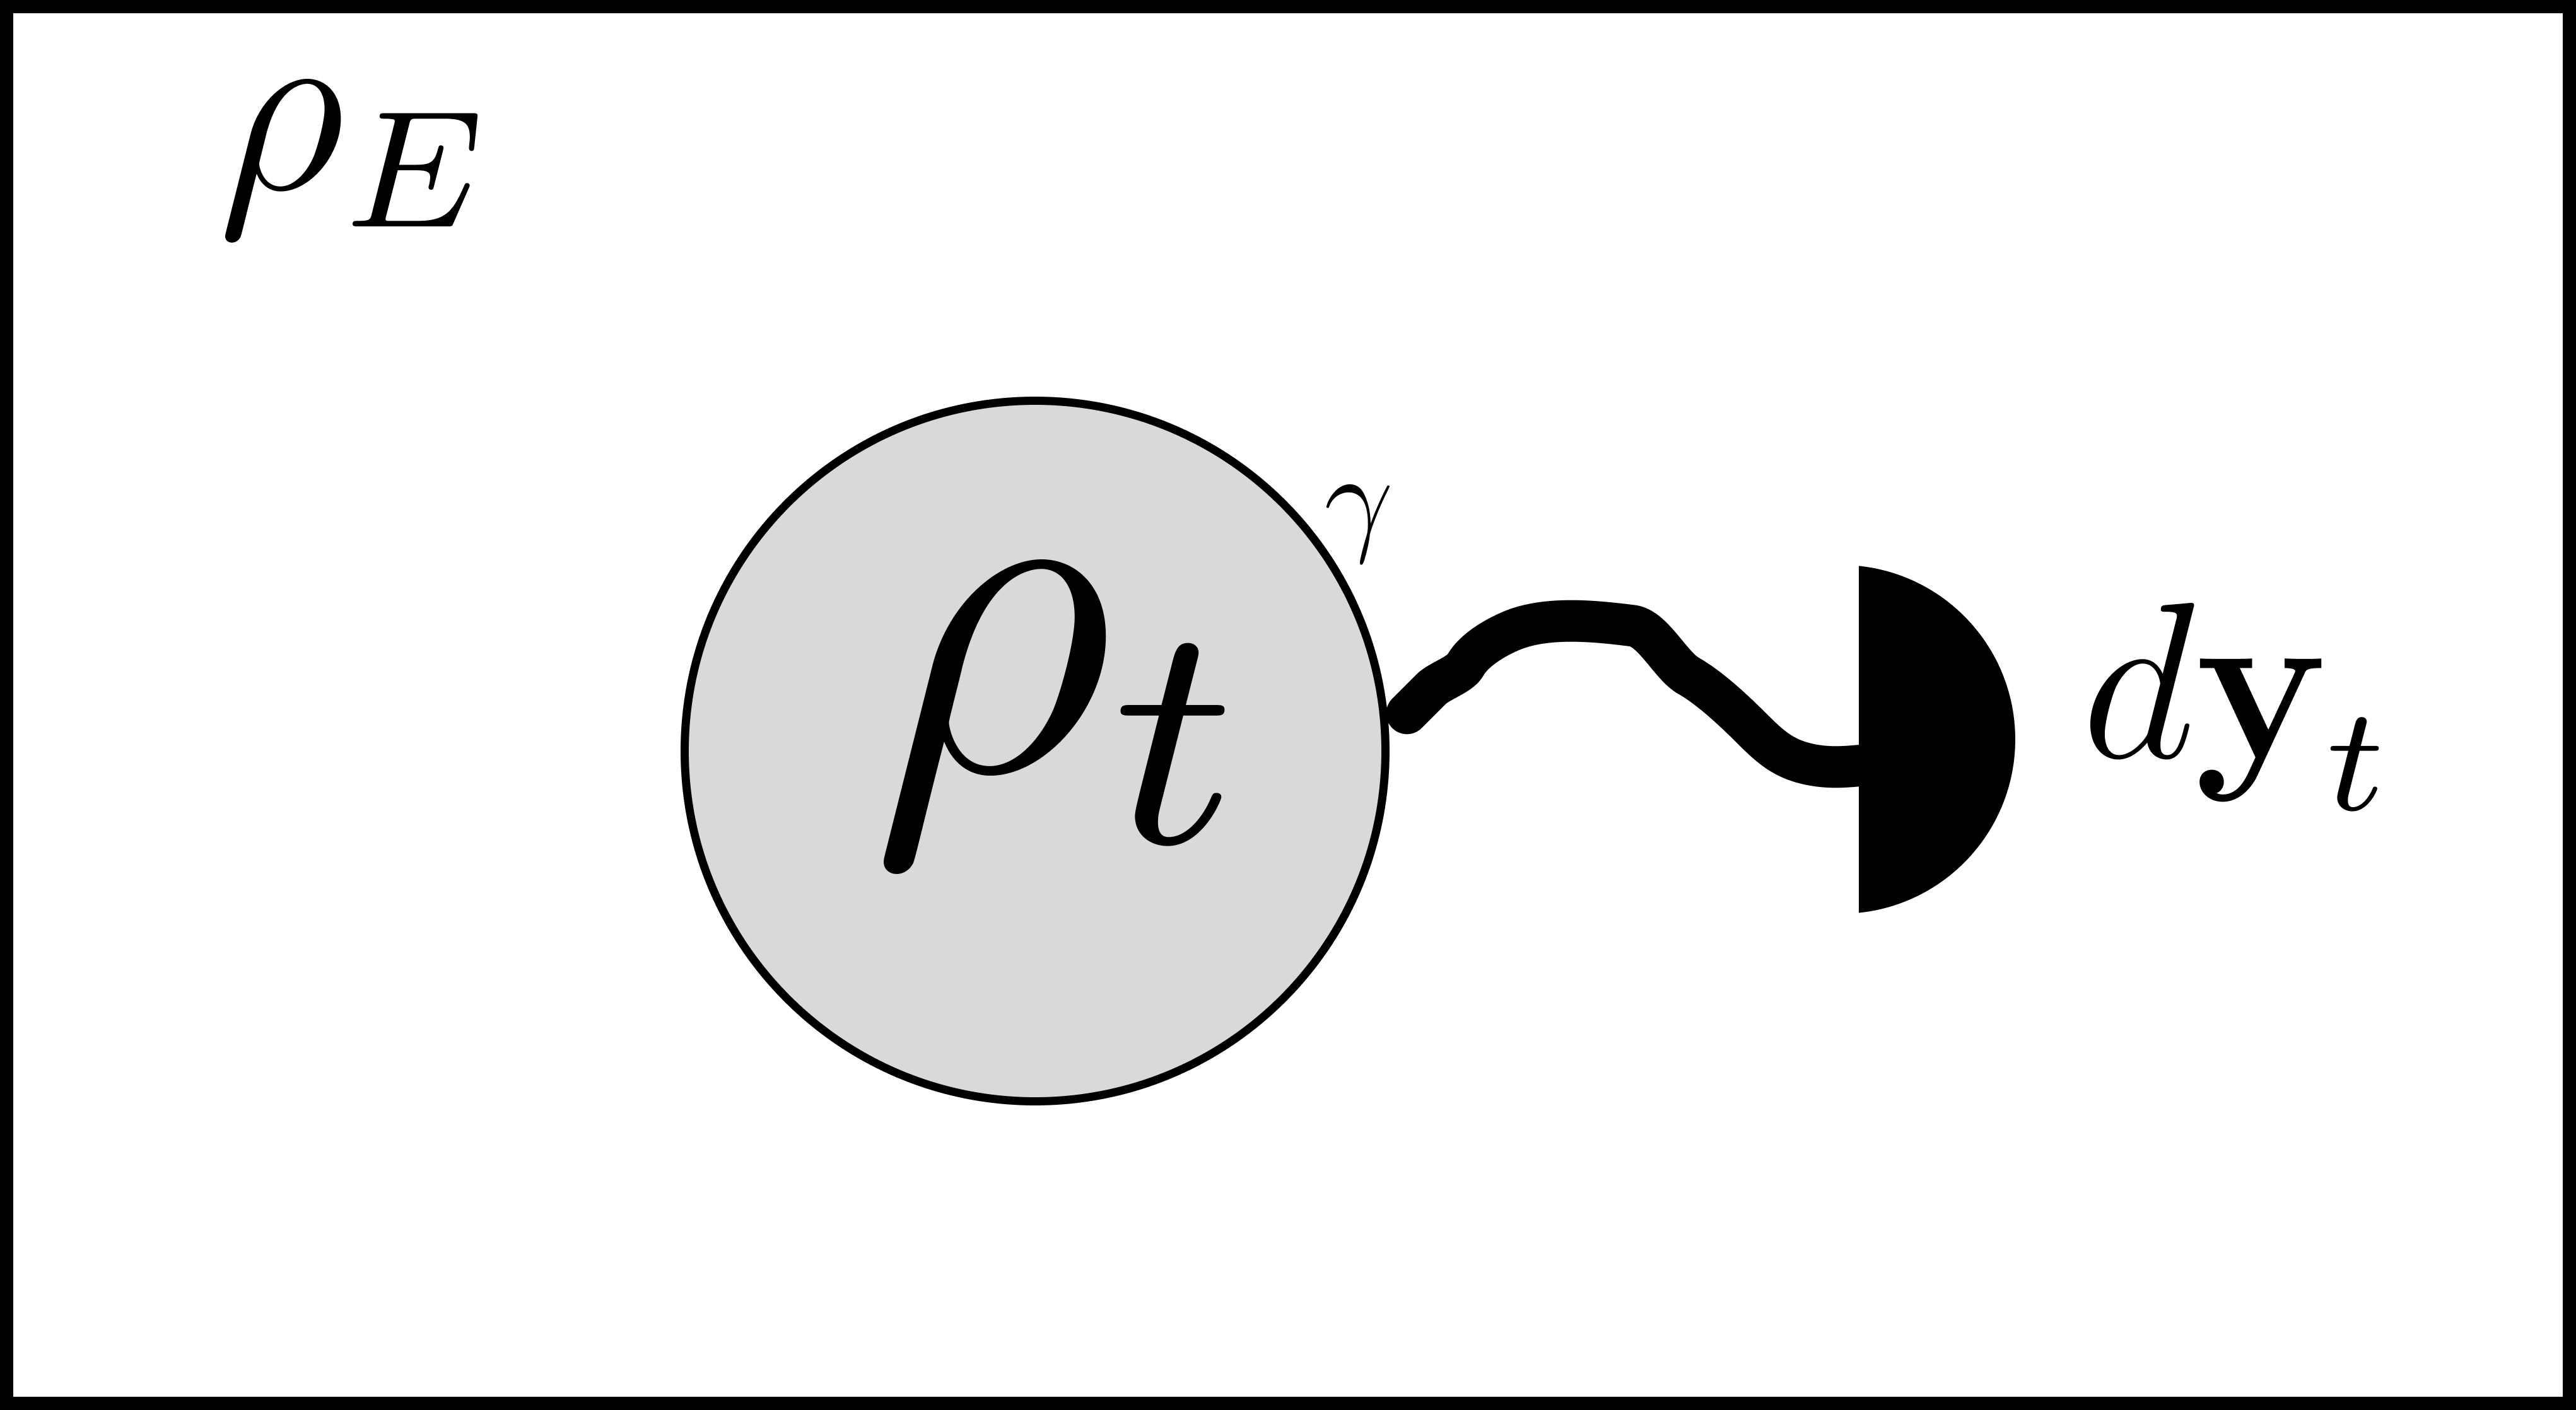
\includegraphics[width=1.\textwidth]{Figures/CMON/INTRO/cmon_esquema.png}
    \caption{We depict the continuously-monitored setting under consideration. This consists on an optomechanical cavity that stores a quantum system $\rho_t$, and whose decay rate is $\gamma$, and is coupled to a bosonic bath $\rho_E$, the latter being constantly measured. This gives rise to the measurement signal, whose (stochastic) value at time $t$ is denoted by $\dyt$.}
    \label{fig:cmon_scheme}
\end{figure}

The most direct way to implement a continuous measurement on a quantum system is to couple it an electromagnetic auxiliary mode that is subsequently measured via photon-counting or homodyning measurements as shown in Fig.~\ref{fig:cmon_scheme}. While several phyiscal scenarios allow for this kind of detection --- among them atomic sensors~\cite{Jimenez2018signal} and mesoscopic electrometers using quantum dots~\cite{Lu2003}---, we will focus on optomechanical cavities~\cite{Aspelmayer2014cavity}.

To this end, we begin in Sec.~\ref{ssec:1_cmon_physics} by providing some insight on optical cavities and their interplay with measurements done on the light that leaks otu of the cavity. Since such measurement outcomes are stochastic, the evolution of the system will be given by a \textit{stochastic master equation} (SME). Thus, in Sec.~\ref{ssec:contphoto} we derive an SME for the case of a single optical mode stored in the cavity and photon-detection done on the outside modes, leading to a SME driven by point processes, \textit{e.g.} the measurement record is a sequence of photon clicks. We then consider homodyne detection in Sec.~\ref{ssec:1_cmon_homodyne}, where the measurement signal becomes continuous, and a Wiener noise appears in the play. Next, a general equation for a continuously-monitored Gaussian system is discussed in Sec.~\ref{ssec:1_cmon_gaussian}.
Finally, in Sec.~\ref{ssec:1_cmon_model} we introduce the optomechanical model that we consider in Chapter~\ref{chapter:CMON}, which is used as a testbed for our approaches to the statistical inference problems considered in that Chapter.

\subsection{Cavity emission and photon-detection}\label{ssec:1_cmon_physics}
Optical cavities consist on convex mirrors faced together at some distance, where light can be stored in a standing wave mode for long periods of time. In order to access the cavity mode, one of the mirrors can be made slightly transmissive, as in Fig.~\ref{fig:cavityCMON}. This allows to retrieve information by measuring the leaked photons and to pump the cavity field by an external laser. Since light is trapped inside the cavity for long periods of times, placing a quantum system inside it, is one of the most effective means of coupling quantum systems to light.

The leaked light occupies travelling modes (free propagating), which means that such photons will never interact again with the system. This fact allows one to describe the evolution of the cavity mode as a Markovian dynamics. This corresponds to an electromagnetic (bosonic) cavity mode coupled to a bosonic bath, which in turn consists in the free-propagating modes. For optical modes, this bath is taken to be at zero temperature, \textit{i.e.} the vaccuum state, but the formalism also allows us to consider non-zero temperatures, that are present for example in the baths of optomechanical systems.

\begin{figure}[t]
    \centering
    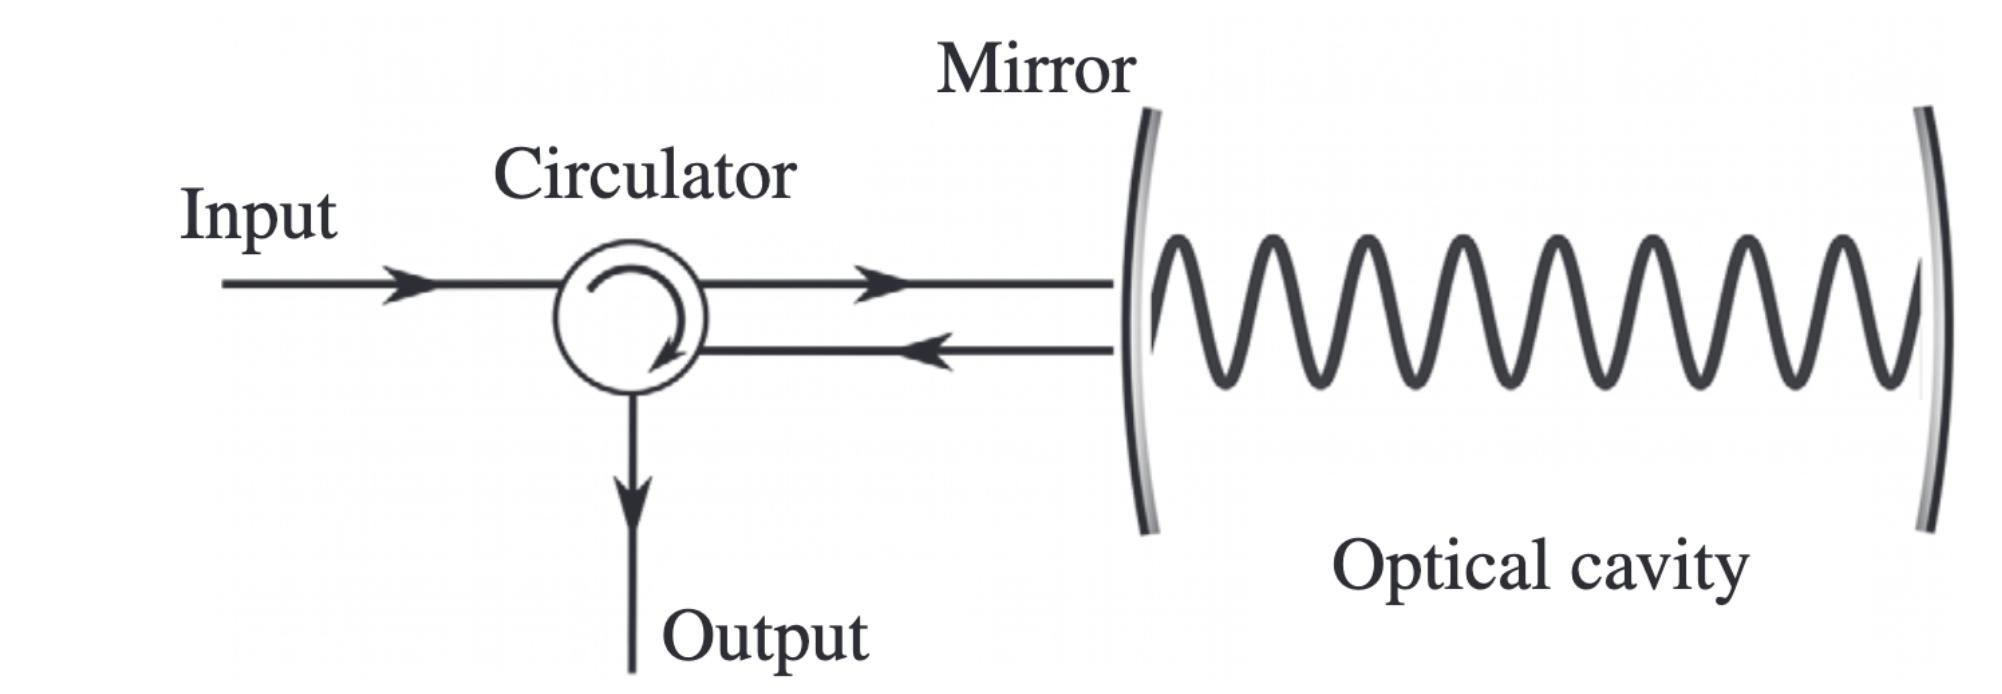
\includegraphics[width=1.\textwidth]{Figures/CMON/INTRO/cavitiy_jacobs.png}
    \caption{An optical cavity is depicted (image taken from Ref.~\cite{jacobs_2014}, Ch.3). Here, light is input (and output) to (and from) the cavity by the same mirror, and such two modes are splitted by the circulator.}
    \label{fig:cavityCMON}
\end{figure}

We denote the cavity's decay rate by $\gamma$ (depending on the transmissivity of the mirror), the annihilation operator for the cavity mode by $a$, and the anhilliation operator at detection time $t$, by $b_t$. By approximating the bath's autocorrelation function as a delta-function, which makes the bath Markovian\footnote{This matter is discussed further in Sec.3.3. and Sec.3.11 of Ref.~\cite{wisemanbook}} we obtain the following commutation for the bosonic bath's operators in the interaction picture w.r.t. system's Hamiltonian:%~\cite{wisemanbook,wiseman1993interpretation,gardiner1985input}
\eq{commbathdelta}{\comm{b_t}{b_{t'}^\dagger} = \delta(t-t').}
Under the rotating-wave approximation, the interaction potential between cavity and bath is modelled to be
\eq{eee}{V_{IF} = -\ii \sqrt{\gamma}\big( b_t a^\dagger - b_t^\dagger a \big),}
and describes the exchange of excitations between each other. However, due to the singularity appearing in Eq.~\ref{eq:commbathdelta}, we must be careful when studying the dynamics generated by $V_{IF}$. A convinient approach is that of interpreting $b_t$ \textit{a la Ito}~\cite{wiseman1993interpretation}\footnote{Ito calculus is a tool of stochastic calculus, that allows to compactly write differential equations for random variables subject to Wiener noise, and also integrals. While working with Ito calculus, one proceeds similarly than traditional calculus but taking into account a few important rules. We briefly discuss this topic in Sec.~\ref{ssec:ito}.}. Thus, an infinitesimal operator is defined as
\eq{infidB}{dB_t = b_t dt,}
where $dt$ accounts for an infinitesimal time-interval leading to $\delta(0)dt = 1$. With the new operators, we then get the following commutation relations:
\equ{\comm{dB_t}{dB_t^\dagger} = dt,}
which indicates that the operator $dB_t$ can be undestood as being order $\sqrt{dt}$. With the re-defined bath's operators, we can now study how an infenitesimal evolution looks like. Here, we must be careful when performing expansions, since the $\sqrt{dt}$ scaling requires to go up to second order terms. To do this, we consider the infinitesimal evolution generated by $V_{IF}$ in Eq.~\ref{eq:eee}, and we get
\begin{align}
U(t+dt,t) &= e^{\sqrt{\gamma}(a \; dB_t^\dagger - a^\dagger dB_t)} \nonumber\\
&= \mathbb{I} + \sqrt{\gamma} \big( a  \; dB^\dagger - a^\dagger dB\big) - \frac{1}{2} \gamma a^\dagger a \;dt - \frac{\gamma}{2}\llaves{a^\dagger, a} dB^\dagger dB  \\ & \spacee+\frac{\gamma}{2} \big(a^2 {dB^\dagger}^2 + {a^\dagger}^2 dB^2\big) \nonumber,
\end{align}
which describes an infinitesimal evolution of the joint system, in the interaction picture.

We will now assume that the bosonic bath is always found in the ground-state $\ket{0}$, and that at each time-step $t$, the system interacts with a new copy of such ground-state, \textit{i.e.} with a new mode $b_t$. Let us also assume that system's state is given by $\ket{\psi(t)}$. With this, the global state at time $t+dt$ is given by
\equ{U(t+dt,t)\ket{0}\ket{\psi(t)} = \Big(\mathbb{I} - \frac{\gamma}{2}a^\dagger a dt\Big)\ket{0}\ket{\psi(t)} + \gamma dB^\dagger \ket{0} a \ket{\psi(t)}.}
Under these assumptions, the probability of finding an excitation in the bath is given by
\equ{p_1(dt) = \gamma \langle 0 | dB dB^\dagger |0\rangle \bra{\psi(t)} a^\dagger a \ket{\psi(t)},} which turns out to be small if we recall that $dB dB^\dagger = dt$.\footnote{This relationship holds since we only keep the non-normally ordered operators in bath's commutation relations, as such is assumed to be in the ground-state}

We also note that if we \textit{do measure} the state of the leaked mode, and detect a photon, the state of the cavity becomes $\ket{\psi_{1}(t+dt})\propto a \ket{\psi(t)}$ (a photon-subtracted state), while if no photon is detected $\ket{\psi_{0}(t+dt)}\propto (\mathbb{I} + \frac{\gamma}{2}a^{\dagger}a)\ket{\psi(t)}$.
In the next section we formalize this (stochastic) conditional state dynamics using a sequence of quantum instruments aplied one  infinitesimal step after the other.

\subsection{Continuous photon-detection}\label{ssec:contphoto}

To begin our study of conditional post-measurement states, we will consider the photon-detection example outlined in the previous section, but we will also include the action of the system's hamiltonian. By
direct identification of the post-measurement (unnormalized) conditional states are given by
$\ket{\psi_0(t+dt)} =M_{0}\ket{\psi(t)}$ and $\ket{\psi_1(t+dt)} =M_{1}\ket{\psi(t)}$  where the two
 Krauss operators are:
\begin{align}\label{eq:photocoM}
M_0 &= \mathbb{I} - \Big(\frac{R}{2} + \ii H \Big) dt\\
M_1 &= c \sqrt{dt},
\end{align}
where $H$ stands for the system's Hamiltonian\footnote{We will drop the hat notation in this Section.}, $dt$ is an infinitesimal amount of time, $c = \sqrt{\gamma}a$, with $\gamma$ being the cavity's decay rate and $R=c^\dagger c$.

By droping terms of $\mathcal{O}(dt^2)$, it is straightfoward to check that $\llaves{M_0, M_1}$ constitute a valid quantum instrument $(M_0^\dagger M_0 + M_1^\dagger M_1 = \mathbb{I})$, and the unconditional post-measurement state, \textit{e.g.} the state of the system at time $t+dt$ when not recording the measurement outcome, recovers the Lindblad form in Eq.~\ref{eq:libland} for the cavity emission model:
\begin{align}\label{eq:cavityemission}
\rho(t+dt) &= M_0 \rho M_0^\dagger + M_1 \rho M_1^\dagger \\
&= \rho - \ii \left[ H,\rho \right] dt + c^\dagger \rho c - \frac{1}{2}\llaves{c^\dagger c, \rho},
\end{align}
If we do keep track of the measurement record, at each (infinitesimal) time step we can get a detection
``click'' (outcome $i=1$) with probability
\eq{pointpro}{p_1(dt) = \tr{\rho M_1^\dagger M_1} = \tr{\rho c^\dagger c} dt.}
and the absence of a click (outcome $i=0$) with probability
\eq{pointpro2}{p_1(dt) =\tr{\rho M_0^\dagger M_0} = 1-\tr{\rho c^\dagger c} dt.}
and the corresponding normalized states will be given by.~\ref{eq:photocoM} we have
\begin{align}
\ket{\psi_1(t+dt)} &= \frac{M_1\ket{\psi(t)}}{|| M_1\ket{\psi(t)}||}=\frac{c_1 \ket{\psi(t)}}{\sqrt{\bra{\psi(t)} c^\dagger c\ket{\psi(t)}}},\\
\ket{\psi_0(t+dt)} &= \frac{M_0\ket{\psi(t)}}{|| M_0\ket{\psi(t)}||}=\frac{1}{\sqrt{ \expect{M_0^\dagger M_0}}} \Big[\mathbb{I} - (\frac{R}{2} + \ii H) \ket{\psi(t)}\Big] \\ \nonumber
&\simeq \Big( 1 + \frac{\expect{c^\dagger c}}{2} dt\big) \Big[ \mathbb{I} - \Big(\frac{R}{2} + \ii H dt\Big)\Big] \nonumber \\
&= \Big(\mathbb{I} - dt\Big[ \ii H + \frac{R - \expect{R}}{2}  \Big] \Big) \ket{\psi},
\end{align}
where we have Taylor-expanded the normalization term in $\ket{\psi_0(t+dt)}$ up to the first order, and dismissed terms $\mathcal{O}(dt^2)$. We that while most of the time the system will evolve continuously with ($M_{0}=\id + \mathcal{O}(dt)$), with very small probability, $p_{1}=\mathcal{O}(dt)$, the state will suffer a very drastic (finite)  change, the so-called \textit{quantum jump}. Note that in both cases, upon a click or a no-click, the act of measuring has always a \emph{back-action} on the system dynamics.


Now we wish to express the above results describing the stochastic evolution of the system in a single stochastic differential equation. For this purpose, we define the stochastic variable $N(t)$, corresponding to the total number of clicks until time $t$,  \textit{i.e.} the number of occurrences of  measurement outcome $i=1$ registered up to time $t$. Since such quantity can only increase by a single unit, the following properties hold:
\begin{align}\label{eq:pointpro}
dN_t^2 &= dN_t \\
\mathbb{E}\corch{dN_{t}} &= \tr{M_1^\dagger(t) M_1(t) \rho(t)} = dt \bra{\psi(t)}c^\dagger c\ket{\psi(t)},
\end{align}
A variable $N(t)$ with these properties defines what is called a \textit{a point process}~\cite{Dolinar1973,wisemanbook}. Since such variable $dN$ can only take the binary values of zero and one, we can compactly write the conditional evolution of the (normalized) pure state as
\eq{condicompa}{\ket{\psi(t+dt)} = \big(1-dN) \corch{\mathbb{I} - \Big(\ii H + \frac{c^\dagger c - \expect{c^\dagger c}}{2}\Big)dt} \ket{\psi(t)} + dN \frac{c\ket{\psi}}{\sqrt{\expect{c^\dagger c}}},}
where the time-dependence of the variable $N$ will be left implicit from now on. This a non-linear, stochastic equation, known as a \textit{Stochastic Scrhodinger Equation} since it preserves the purity of the state. Any solution to this equation defines a quantum trajectory,
and describes the possible paths that the quantum state can take under the stochastic outcomes obtained from the point process.
By dropping the terms of order $dN dt$\footnote{this can be justified by the fact that the probability of $dN=1$ is of order $dt$}, we get
\eq{sse}{\ket{\psi(t+dt)} = \ket{\psi} + dN\Big( \frac{c}{\sqrt{\expect{c^\dagger c}}} - 1\Big) \ket{\psi} + \frac{1}{2}dt \Big( c^\dagger c - \expect{c^\dagger c} - 2\ii H\Big) \ket{\psi}.}

We can now extend this to density matrices by witting $\rho(t)=\proj{\psi(t)}$ and  dropping high order terms in $d$t:
\begin{align}\label{eq:foto}
d\rho = dN \Big(\frac{c \rho c^\dagger}{\expect{c^\dagger c}}\Big) - dt \Big( \ii \comm{H}{\rho} + \frac{1}{2}\llaves{c^\dagger c, \rho} - \frac{1}{2}\expect{c^\dagger c} \rho\Big).
\end{align}
which by linearity extends to arbitrary mixed initial states. Note that averaging this equation out over all possible measurement outcomes and recalling $\mathbb{E}\corch{dN_{t}} =\expect{c^\dagger c}$ one recovers again  the Lindbladinan dynamics.

This can also be written as
\begin{equation}\label{eq:nav1}
d\rho(t) = \; dN \Goc\rho(t) -\; dt \mathcal{H}\Big[\ii H + \frac{c^\dagger c}{2}\Big] \rho(t),
\end{equation}
in terms of the super-operatos $\mathcal{G}$ and $\mathcal{H}$ as
\begin{align}\label{eq:superGH}
\Goc \rho &= \frac{c \rho c^\dagger}{\expect{c^\dagger c}}\\
\Hoc \rho &= c \rho + \rho c^\dagger - \tr{\rho(c + c^\dagger)} \rho
\end{align}

We note that one could easily extend this approach to include consider more \textit{jump operators}, $\llaves{c_i}_{i=1}^M$ by taking $M_i = c_i \sqrt{dt}$,  $M_0 = \mathbb{I}- (\frac{R}{2} + \ii H) dt$ with $R=\sum_{i=1}^M c_i^\dagger c_i$. For example, one could include losses the other mirror. Most interestingly, this approach lets us easily describe situations in which only some types of jumps are monitored or accounted for. One then obtains a stochastic equation with jump terms of the form $G[c]$ for the monitored modes and the averaged Lindbladian counterpart for the unobserved modes.

In this section we have studied the conditional evolution of system under the particular measurement choice in Eq.~\ref{eq:photocoM} (corresponding to photon-counting), and we have obtained the
stochastic equation describing the continuously monitored system. As discussed in the introduction to quantum channels and quantum instruments, for a fixed interaction between the system and the auxiliary system, different choices of measurement on the auxiliary system lead to different Kraus representations of the same quantum map.  In the next section we will study the conditional dynamics when one performs a different a different type of measurement on the auxiliary (bath) modes. Of course, this will lead to a completely different type of stochastic equation, but if we average over all its realization we will recover the same Lindblad equations.

The different stochastic differential equations corresponding to the same average open system Lindbladian equations are called \textit{unravelings}. We remark here that while in many works these unravellings are presented as just convenient interpretations or as a numerical  tool to simulate (Montecarlo) open system dynamics ---in many occasions it is much simpler to propagate the pure state, than the full density matrix---, in this thesis the particular unravelling will have a direct physical meaning and we will be concerned about inference methods based the single-trajectories, single (possibly long) measurement records rather than average quantities of the state.

\subsection{Continuous homodyne detection}\label{ssec:1_cmon_homodyne}
We have previously study an stochastic master equation for an specific \textit{unraveling} of unconditional dynamics, namely photon-detection. In such case, a detection induces a \textit{quantum jump} on the system's density matrix, with a probability that is proportional to $dt$, as given by Eq.~\ref{eq:pointpro}. Here, we will study a different unraveling of the dynamics.

The existence of different unravelings arises from the invariance of the master equation --- \textit{i.e.} the undonditional open quantum system dynamics revisted in Sec.~\ref{ssec:1_intro_open} --- under certain transformations (see also Eq.~\ref{eq:invalibland}) of the form
\begin{align}
c &\rightarrow c + \alpha \\
H &\rightarrow H - \frac{\ii}{2}\big(\bar{\alpha}c - \alpha c^\dagger),
\end{align}
with $\alpha \in \mathbb{C}$. This is (unitarily equivalent) to a different set of Krauss representation:
\begin{align}\label{eq:homPOM}
M_0 &\rightarrow\tilde{M}_0(t) = \mathbb{I} - dt\Big(\ii H + \frac{\bar{\alpha}c - \alpha c^\dagger - (c+\alpha)^\dagger(c+\alpha)}{2}\Big) \\
M_1  &\rightarrow \tilde{M}_1(t) = \sqrt{dt}(c+\alpha).
\end{align}
This transformation can physically be achieved by mixing the input field with a strong local oscillator (L.O.) by a low transmissivity beam-splitter (BS)\footnote{To see this, let the transmissivity of the BS be $\eta\sim1$, and let the intensity of the L.O. be $\frac{\alpha}{\sqrt{1-\eta}}$; the reflected mode will then be \equ{\sqrt{\eta} c + \alpha,}assuming we treat the local oscillator classically, an approximation valid when the intensity of the L.O. is sufficiently high~\cite{serafiniBOOK}. From here, since $\sqrt{\eta}\sim1$, we get the desired transformation.}, as shown in Fig.~\ref{fig:direhom}, which corresponds to direct homodyne detection. In turn, let us restrict to $\alpha\in\mathbb{R}$, then a detection (as defined in the previous section) happens with probability
\begin{align}
p_1(dt) = \mathbb{E}\corch{dN} &= \tr{\rho (c+\alpha)^\dagger(c+\alpha)} dt \\
&= \tr{\rho \big(c^\dagger c + \alpha (c+c^\dagger) + \alpha^2\big)}\\
&= \tr{\rho \big(c^\dagger c +  \alpha q + \alpha^2\big)},
\end{align}
where $q = c+c^\dagger$ stands for the position quadrature\footnote{We will momentaneously drop the $\sqrt{2}$ factor to ease the notation}. Thus, if $\alpha\gg\expect{c^\dagger c}$, photon-detection at the reflected port is equivalent (up to a constant) to measuring the $q$ quadrature. This is corresponds to the case of direct \textit{homodyne} detection, which was introduced in Sec.~\ref{ssec:1_cv_measurements}; we will here consider the direct homodyne detection, which is realized by mixing the system with a strong local oscillator by a low transmissivity beam-splitter, as shown in Fig.~\ref{fig:direhom}.

\begin{figure}[t!]
    \centering
    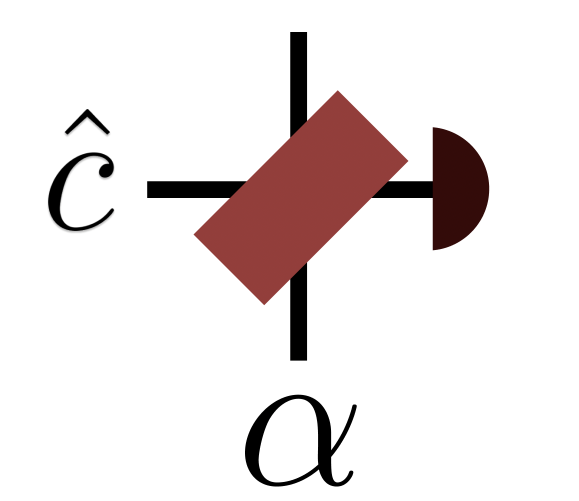
\includegraphics[width=0.35\textwidth]{Figures/CMON/INTRO/homosimpl.png}
    \caption{We sketch a direct homodyne detection. The beam-splitter is chosen such that the reflected part (which is subsequently measured) has only a small contribution of the local oscillator, and is dominated by the original signal associated to the system we are measuring.}
    \label{fig:direhom}
\end{figure}

Repeating the same procedure outlined by the end Sec.~\ref{ssec:contphoto}, but now with the transformed set of Krauss operators $ \llaves{\tilde{M}_0(t), \tilde{M}_1(t)}$, we get an stochastic master equation that reads
\begin{align}
d\rho = \mathcal{G}[c+\alpha] \rho dN + dt \mathcal{H}\Big[\ii H + \alpha c + \frac{c^\dagger c}{2}\Big].
\end{align}
From here, we aim to take the continuous limit, in which the photocurrent is approximated by a continuous function of time. This corresponds to the ideal limit of homodyne detection, in which the intensity of the local oscillator goes to infinity. In particular, we are interested in a regime under which the number of detections per time is high and changes in the system are small. In such regime, we obtain a \textit{Belavkin-Zakai} equation, which is yet another quantum stochastic master equation, that describes the continuous homodyne-monitoring of a quantum system. We will now derive such equation by making expansions in terms of the local oscillator intensity, following Ref.~\cite{wisemanbook}\footnote{Note that there are alternative ways to derive this equation. For instance by straightfowardly considering the action of a Gaussian measurement on the quantum state and Taylor-expanding it in terms of $dt$~\cite{jacobs_2014, JacobsStraightfoward2006}, or considering the interaction between a Gaussian system, bath and measurement\cite{serafini2017quantum,Genoni2016conditional}, although this formalism is focused on Gaussian systems, and directly leads to the set of stochastic linear equations for mean and covariance of the quantum state, which we discuss later on, bypassing stochastic master equations.}.

We begin by considering a small time-interval $\delta t = \mathcal{O}(\alpha^{-\frac{3}{2}})\ll1$\footnote{The only purpose of considering $\delta$ rather than $d$ is that we take a limit in terms of local oscillator intensity by the end of this discussion}, that results in an expected number of detections,
\eq{edng}{\mathbb{E}[\delta N] = \delta t\;\tr{\rho (\alpha^2 + \alpha q + c^\dagger c)} = \mathcal{O}(\alpha^{\frac{1}{2}}),}
which is large in comparison to system's evolution (since $\delta t = \mathcal{O}(\alpha^{-\frac{3}{2}})$). Under this choice of scaling, the detection probability is algo large $p_1(\delta t) = \mathcal{O}(\sqrt{\alpha})$.

As pointed out in Sec.~\ref{ssec:1_cv_measurements}, $\delta N$ is a Poissonian random variable. However, it is possible --- since the number of detections happening per $\delta t$ is large --- to approximate such probability distribution by a normal distribution~\cite{wisemanbook,wiseman1993quantum} (intuitively we can understand this as a central-limit theorem) with a mean-value given by Eq.~\ref{eq:edng} and variance
\eq{variaCMON}{\sigma^2= \delta t \big(\alpha^2 + \mathcal{O}(\alpha^{\frac{3}{2}})\big).}
By recurring to Ito calculus, Eq.~\eqref{eq:variaCMON} can be written compactly as
\eq{dnito}{\delta N = \alpha^2 (\delta t) \corch{1 + \frac{\expect{q}(t)}{\alpha}    } + \alpha \delta W,}
where $\delta W$ describes a differential white noise, \textit{e.g.} a zero-mean normal random variable whose variance is $\mathbb{E}[\delta W^2] = \delta t $.

It is now time to make a brief pause, and jump to revise Ito calculus. The interested reader is referred to Ref.~\cite{gardiner2004handbook}, where further details about this topic can be found.

\subsection{Intermezzo II: Ito calculus}\label{ssec:ito}
In a nutshell, Ito provides a tool to tackle problems involving stochastic differential equations,
where the infinitesimal change $dX_{t}$ of a variable $X_{t}$ occurring in an infinitesimal time $dt$ interval is written in terms of deterministic part (proportional to $dt$) and a stochastic infinitesimal increment $dW$.
Here we will focus on processes driven by Wiener noise and Ito calculus will give us tools to make sense of and compute integrals such as $\int X_{t} \; dW$.

A Wiener process $W(t)=\int_{0}^{t}dW$ describes stochastic curve
with zero mean and a variance that grows as $t$, and is defined in such a way that it is \emph{continuous} in time. The infinitesimal Wiener increments $dW$ have zero mean and variance $\mathbb{E}({dW^{2}})=dt$, but in order to guarantee that $W(t)$  is a continuous function, the increments have the (surprising) property that $dW^2=dt$, \textit{i.e.} it is deterministic (the distribution of $\Delta W^2$ become more and more peaked as the time intervals $\Delta t$ smaller). A Wiener process can be thought of as the continuum limit of a random walk or brownian motion

Consider the general (1D) Ito stochastic differential equation
\eq{1_stoch}{dX_t = a(X_t,t) X_t dt + b(X_t,t) dW_t.}
While the coefficientes $a(X_t,t)$ and $b(X_t,t)$ might be arbitrary functions, in case they are state-independent --- known as a drift-difussion process --- an integral expression can be defined as
\eq{1_ou_integal}{X_t = \int_{t_0}^t a(t') dt' + \int_{t_0}^t b(t') dW_{t'},}
where the second integral is an \textit{stochastic Ito integral} (whose value depends on the specific realization of the Wiener process up to time $t$).

Contrary to Riemman integral, when dealing with stochastic integrals it is of utmost importance to choose the value at which to evaluate the function for on each partition, due to the stochastic nature of the resulting function. Ito integral is defined by considering the value that the function takes at the beginning of each partition. For example, in a different stochastic calculus named by Stratonovich, the integral is defined by averaging up the values at the two extremes of the interval, and the rules of calculus are completely different. In this thesis, we will work with Ito integrals.

Here, we observe that $X_t$ clearly does \textit{not} depend on the \textit{future} realisations of the Wiener process (that is, on values $dW_s$ for $s>t$); this captures the notion of a \textit{non-anticipating function of t}, which we denote by $NA(t)$. That is, a stochastic function $G(t)$ is $NA(t)$ if $\forall\;t$ and $\forall \; s$ such that for $t<s$, the values that $G(t)$ take are statistically independent of the future increments $W(s) - W(t)$, with $W(T) = \int_0^T dW_t$.

Given $G(t)$ and $H(t)$ non-anticipating functions, and when integration \textit{a la Ito}, the following holds:
\begin{enumerate}
\item $\expect{\int_{t_0}^tG(t')dW_{t'}} = 0$, which can be seen by the construction of Ito's integral.
\item $\expect{\int_{t_0}^t G(t')dW_{t'} \Big[\int_{t_0}^{t'} H(s') dW_{s'}\Big]} = \int_{t_0}^t \expect{G(t') H(t')} dt'$, which can be understood as a correlator formula, and where $\expect{dW_t dW_s} = \delta_{t,s} dt$ rules the stochastic integration out.
\item $\expect{\int_{t_0}^t G(t')dW_{t'} \Big[\int_{t_0}^{t'} H(s') dW_{s'} \Big]} = 0$, which can be understood from the fact that $\tilde{H}(t') = \int_{t_0}^{t'} H(s') dW_{s'}$ is $NA(t')$ and thus the function $G(t')H(t')$ is $NA(t')$, whose stochastic integral averages to zero (see first item).
\item Let $\tilde{G}$ and $\tilde{H}$ be determinstic functions of time\footnote{This expression finds use when considering, for example, $\tilde{G}$ and $\tilde{H}$ to be diffusion coefficients of respectively different stochastic processes.}, then \equ{\expect{\int_{t_0}^t \tilde{G}(t')dW_{t'} \int_{t_0}^s \tilde{H}(s') dW_{s'}} = \int_{t_0}^{\text{min}(t,s)} dt' \tilde{G}(t')\tilde{H}(t').}
\end{enumerate}
Where we use the $\expect{\cdot}$ notation instead $\mathbb{E}(\cdot)$ for the expected values whenever there's no ambiguity with the expectation over quantum states.

When considering the derivative of a (twice-differentiable) function $f(X_t,t)$, one has to be carefull in not using blindly the chain rule. One needs to take Taylor expand $f$ up to second-order, taking into account that $dW\sim O(\sqrt{dt})$:
\equ{df=\big(\frac{\partial f}{\partial t} + a(t) \frac{\partial f}{\partial x} + \frac{b^2(t)}{2} \frac{\partial^2 f}{\partial x^2}\big) dt + b(t) \frac{\partial f}{\partial x} dW_t.}
The latter formula is known as the \textit{Ito lemma}, and we can understand it as a way to take into account a change of variables when studying the dynamics of a stochastic system.

When the drift $a(t)$ and diffusion $b(t)$ coefficients in Eq.~\ref{eq:1_stoch} are constant, the process is known as an \textit{Orstein-Uhlenbeck process}:
\equ{dX_t = \kappa( \mu - X_t) dt + \sigma dW_t,}
whose solution is easily obtained by a change of variables $Y_{t}= X_{t} e^{\kappa t}$. Using Ito's lemma:
$$dY=\kappa X_{t}e^{\kappa t} dt+e^{\kappa t} dX_{t}=\kappa \mu e^{\kappa t} dt+\sigma e^{\kappa t} dW_{t}$$
from where
$$Y_{t}=Y_{0}+\int_{0}^{t}\kappa \mu e^{\kappa t} dt'+\int_{0}^{t}\sigma e^{\kappa t} dW_{t'},$$
and using  $X_{t}= Y_{t} e^{-\kappa t}$:
\equ{X_{t}=X_{0}+\mu (1-e^{-\kappa t}) +\sigma \int_{0}^{t} e^{-\kappa (t-t')} dW_{t'}}
we get
\equ{X_t = \mu\big(1-e^{-\kappa t}\big) + \sqrt{D}\int_0^t e^{-\kappa(t-t')dW_{t'}}.}
Using the aforementioned rules, we can readily check that, for $t\rightarrow\infty$,
$\mu = \mathbb{E}[X_t]$ and $\text{Var}[X_t]=Dt$, which indicates that the distribution diffuses in time; in turn, this solution corresponds to a Gaussian probability distribution.
The mean and variance of $X_{t}$ can now be readily computed using the integration rules above,

\begin{align}
\expect{X_{t}}&=X_{0} e^{-\kappa t}+\mu(1-e^{-\kappa t}) \xrightarrow{\: t \to \infty \: } \mu \\
\text{Var}[X_t]&= \frac{\sigma^{2}}{2\kappa}(1-e^{-2\kappa t}) \xrightarrow{\: t \to \infty \: } \frac{\sigma^{2}}{2\kappa}
\end{align}
That is, unlike the Wiener process, the mean and variance converge to constant values for large times.
Moreover, since the process is Gaussian, the probability distribution of $X_{t}$ at a given time is a Gaussian with the mean and variance above. In turn, the probability of whole trajectory is fully determined by the first and second moments (including $\expect{X_{t}X_{t'}}$, which can also be readily computed).

The connection between SDE and probability distribution of the variable $X_{t}$ at a given time  can be established for more general processes.
In turn, considering any function $f(X_t)$ where the dynamics of $X_t$ is given by Eq.~\eqref{eq:1_stoch}, we have that
\begin{align}
\frac{\expect{df(X_t)}}{dt} &= \expect{\frac{df(X_t)}{dt}} = \frac{d}{dt} \expect{f(X_t)} \\
&= \expect{a(X_t,t) \partial_x f + \frac{1}{2} b(X_t,t)^2 \partial_x^2 f}
\end{align}
Considering that $X_t$ has a conditional probability density $p(X_t,t|X_0,t_0)$ then
\begin{align}
\frac{d}{dt}\expect{f(X_t)} &= \int dX f(X) \partial_t p(X,t|X_0,t_0) \\
&= \int dX \; \Big[a(X_t,t) \partial_X f + \frac{1}{2} b(X_t,t)^2 \partial_x^2 f\Big] p(X_t,t|X_0,t_0).
\end{align}
Integrating by parts and using the fact that $f(x)$ is arbitrary, we arrive to the \textit{Fokker-Planck} equation
\begin{align}
\partial_t p(X_t,t|X_0,t_0) = - \partial_X\;[a(X,t) p(X,t|X_0,t_0)] + \frac{1}{2} \partial_X^2[b(X,t)^2 p(X,t|X_0,t_0)],
\end{align}
resulting in an analogous description of the process in terms of an differential equation for its probability distribution.

\textit{Fin del intermezzo.}
\vspace{1cm}

Recalling that the evolution of cavity's system under the transformed measurement operators of Eq.~\eqref{eq:homPOM} reads
\equ{\delta \rho = \delta N(t)\mathcal{G}\Big[c+\alpha\Big]\rho - \delta t \mathcal{H}\Big[\ii H + \alpha c + \frac{c^\dagger c}{2}\Big]\rho,}
we can now work the $\mathcal{G}[c+\alpha]$ term and expand it in powers of $\alpha^{-1}$; this means keeping the terms up to $\frac{1}{\alpha^2}$ arising by Taylor expanding up to the second order the normalization in $\mathcal{G}$ (see Eq.~\ref{eq:superGH}). After such expansion, we obtain
\begin{equation}\label{eq:ddynexp}
\delta \rho = \delta N(t) \Big[ \frac{\mathcal{H}[c]}{\alpha} + \frac{\mathcal{G}[c] - \expect{q} \mathcal{H}[c]}{\expect{c^\dagger c}} \Big] \rho - \delta t \mathcal{H}\Big[\ii H + \alpha c + \frac{c^\dagger c}{2}\Big]\rho
\end{equation}
Now, plugging the Ito form of $\delta N$ into Eq.~\ref{eq:ddynexp}, we get
\begin{equation*}
\delta \rho = \Big( \alpha^2 \delta t \Big[ 1 + \frac{\expect{q}}{\alpha}\Big] + \alpha \delta W \Big) \Big( \frac{\mathcal{H}[c]}{\alpha} + \frac{\mathcal{G}[c]\expect{c^\dagger c} - \expect{q}}{\alpha^2} \Big)
\rho + \delta t \mathcal{H}\Big[-\ii H - \alpha c - \frac{c^\dagger c}{2}\Big]\rho.
\end{equation*}
From here, we can expand all the products on the above equation and keep terms of order $\frac{1}{\sqrt{\alpha}}$ or higher. Finally, taking the limit $\alpha\rightarrow \infty$ we get the desired Belavkin-Zakai equation for homodyne measurement:
\begin{align}\label{eq:1introBELAVKIN}
d\rho &= dt\Big(- \ii \Comm{H}{\rho} + \mathcal{D}[c]\rho\Big) + \mathcal{H}[c]\rho \;dW\\
\mathcal{D}[c]\rho &= c\rho c^\dagger - \llaves{\frac{c^\dagger c}{2},\rho} \\ \nonumber
\mathcal{H}[c]\rho &= c\rho + \rho c^\dagger - \tr{(c+c^\dagger)\rho},\nonumber
\end{align}
where to facilitate reading we included the definitions of the super-operatos $\mathcal{D}[c]$ and $\mathcal{H}[c]$ introduced before.

The last equation describes the evolution of a Markovian system which is subject to a continuous monitoring under homodyne detection. As a consequence, the so-called \textit{back-action} term arises (the one accompanying the Wiener noise), which takes into account the effect measurement result recording. Similar to photon-detection situation, when averaging out over possible measurement outcomes, the Lindblad form is recovered.% (\textit{i.e.} the non-selective master equation).

On the other hand, a measurement \textit{signal} arises, which is also a continuous function of time. To see this, let us return to the Ito expression for $\delta N(t)$, namely
\equ{\delta N(t) = \alpha^2 \delta t \left[ 1 + \frac{\expect{q}(t)}{\alpha}\right] + \alpha \; \delta W,}
which after substracting the intensity of the local oscillator we get
\begin{equation}
dy(t) = \underset{\alpha \rightarrow \infty}{\text{lim}} \frac{\delta N (t) - \alpha^2\delta t}{\alpha} = \expect{q}dt + dW,
\end{equation}
where clearly $\expect{q}$ is time-dependent and also the Wiener noise. As we will later see one can use this equation to replace de Wiener term in stochastic equation \eqref{eq:1introBELAVKIN} by $dW=dy-\expect{q}dt$ to obtain the conditional quantum state of the system given a homodyne measurement record.

Overall, we have seen one gets very different kind of information about the cavity mode from the information that has leaked from it, when we mix the leaked light with a local oscillator before the detector instead of measuring leaked light directly with a photo-detector (in-phase quadrature vs. photon number). We also note that the nature of the measured signal is very different: for homodyning we obtain essentially a continuous noisy signal while for photo-counting one gets a sequence of sparse sequence of ``clicks''. Similarly, the stochastic equation describing the system is of a very different nature: in the first case it's a smooth diffusion-type equation, while in the later exhibits abrupt quantum jumps. Of course, both lead to the same master equation when the leaked photons are traced out (or equivalently when all conditional dynamics is averaged out).

In the next Section we briefly explain how to take into account detection inefficiencies.

\subsection{Imperfect detection}
First, the case of inefficient detection, in which the efficiency of the photodetector $\eta$ is less than unity. In this case, the master equation describing cavity emission of Eq.~\ref{eq:cavityemission} can be understood as
\begin{align}
d\rho = -\ii \Comm{H}{\rho}dt + (1-\eta)\mathcal{D}[c] \rho dt + \eta \mathcal{D}[ c]\rho,
\end{align}
and only unravel the last term\footnote{note that $\mathcal{D}[\sqrt{\eta} c] = \eta \mathcal{D}[c]$.}, resulting in a modified stochastic master equation that for the homodyne case Eq.~\ref{eq:1introBELAVKIN} is slightly modified to read
\begin{align}\label{eq:inefficientDETECTION}
d\rho = -\ii\comm{H}{\rho}dt + \mathcal{D}[c] \rho dt + \sqrt{\eta} \mathcal{H}[c] \rho \;dW.
\end{align}
Moreover, the homodyne measurement signal for the inefficient detection case reads
\begin{align}\label{eq:1_cmon_ineff_measu}
dy = \sqrt{\eta} \langle q \rangle dt + dW.
\end{align}

The remaining refinement that we consider deals with the bosonic bath, which so far has been assumed to be in the ground-state. However, we might assume that the cavity is in contact with a thermal bath. Deriving stochastic master equations when measuring such thermal bath turns to be an obscure subject~\cite{wisemanbook,jacobs_2014}. However, we can assume that the thermal bath is just an extra reservoir which we do not measure. In this case, we recall that the master equation (for the cavity plus thermal bath only) reads:
\begin{align}\label{eq:master_thermal}
\frac{d\rho}{dt} = -\ii\Comm{H + \ii(\bar{\beta} c + \beta c^\dagger)}{\rho} (n_{th}+1) + \mathcal{D}[c] \rho + n_{th} \mathcal{D}[c^\dagger] \rho,
\end{align}
where $n_{th}$ is the average number of photons in the cavity and depends on bath's temperature, and we observe that the mean value of the incoming field, $\beta dt = \expect{dB}$, has a driving effect on the cavity\cite{wisemanbook}. This driving term induces a constant shift in cavity's quadratures that in the following will be dismissed.

As stressed in Sec.~\ref{sec:1_cv}, measuring system's quadrature belongs to the set of Gaussian measurements, and as such preserves the gaussian character of (an initially gaussian) state. This motivates the following Section, in which we study the quadratures dynamics of a quantum system under continuous homodyne detection.

\subsection{The Gaussian case}\label{ssec:1_cmon_gaussian}
In the previous Sections we have studied the dynamics of a cavity when its bath is being continuously-monitored, and also discussed a model for imperfect detections. We will now discuss the dynamics structure when the system is assumed Gaussian. We have introduced Gaussian systems in Sec.~\ref{ssec:intro_cv_gaussianinfo}, and also studied how a Gaussian map modifies the first moments of a Gaussian state in Sec.~\ref{ssec:1_cv_channels}. Opposite to such Section, we are here interested in studying the \textit{conditional} diffusive dynamics of the Gaussian system, arising as a consequence of continuously-monitoring the bath coupled to it.

Our discussion follows \textit{the Wiseman approach}~\cite{wisemanbook,Wiseman2005optimal,wiseman1993interpretation}, which consists on deriving dynamical equations for the moments of a Gaussian state \textit{from} the stochastic master equation of Eq.~\ref{eq:1introBELAVKIN}. However, we remark that for the Gaussian case, the same equations can be derived by straightfowardly working with the moments, and assuming an specific (Gaussian) structure for the interaction between bath's and system's modes. This constitutes the \textit{Serafini approach} one, and while it will not be discussed here, the interested reeader can consult Refs.~\cite{serafiniBOOK,Genoni2016conditional}.

For the sake of simplicity, we will restrict to a single-mode quantum system. We consider an equation of the form in Eq.~\ref{eq:1introBELAVKIN}:\footnote{Let us remark that while we derived such equation for an optical cavity, it can be used to describe more complex systems, such as quantum dots coupled to nano-mechanical resonators~\cite{wisemanbook}. Morever, by the end of this Section we will consider a slightly more complex model for the cavity, and discuss an scenario where a mechanical mode is also considered.}
\begin{align}\label{eq:cmon_optimal1}
d\rho &= \mathcal{L}_0 \rho dt + \mathcal{H}[c]\rho \; dW_t,
\end{align}
where $c$ is an arbitrary system operator ($c=\sqrt{\gamma}a$ in the cavity model), and $\mathcal{L}_0$ is the Lindbladian describing the non-diffusive open-quantum dynamics (that takes into account interaction with additional modes).

We recall that Gaussian states are generated by Hamiltonians which are at most quadratic in system's quadratures:
\begin{align}
H = \frac{1}{2} \rop G \rop - \rop^T \Omega B \textit{u}(t),
\end{align}
where $G$ is the Hamiltonian matrix (\textit{i.e.} $G$ is real and symmetric)\footnote{Note our change in notation with respect to Sec.~\ref{sec:1_cv}, \textit{e.g.} $G\equiv H$ in Eq.~\ref{eq:hamiGauss}.} and included a possible time-dependent drive $\textit{u}(t)$ that enters in the Hamiltonian as a linear term (\textit{e.g.} a displacement due by a driving force). Also, we recall that $\Omega$ is the symplectic form defined in Eq.~\ref{eq:cv_ccr}, and that system's mean and covariance are defined as $\rbar = \expect{\rop} = \tr{\rho \rop}$ and $\cov_{nm} = \expect{\Delta \rop_n \Delta \rop_m} + \expect{\Delta \rop_m \Delta \rop_n}$, with $\Delta \rop_i = \rop_i - \expect{\rop_i}$, and $\rop = (q, p)$.
Moreover, the transformation $\tilde{C}$ mapping system's quadratures with the operator $c$ in Eq.~\eqref{eq:cmon_optimal1} is defined via $c = \tilde{C} \rop$, which for the cavity model reads $\tilde{C}=\sqrt{\gamma}\Big(1, \ii\Big)$.

If we only consider the unconditional dynamics, given by the Lindbladian $\mathcal{L}_0$, and use the canonical commutation relations in Eq.~\ref{eq:cv_ccr}, we can derive a dynamical equation for the first two moments $\rbar, \cov$:
\begin{align}\label{eq:cmon_unco}
d \rbar &= \Big(A\rbar  + B\textit{u}(t)\Big) dt\\
d \cov &= \Big(A \cov + \cov A^T + D \Big) dt, \nonumber
\end{align}
where $A = \Omega( G + \text{Im}[\mathcal{C}])$ and $D = \Omega \text{Re}[\mathcal{C}]\Omega^T$ and $\mathcal{C} = \tilde{C}^\dagger \tilde{C}$~\cite{Wiseman2005optimal}. We note that Eq.~\ref{eq:cmon_unco} is just a different parametrization of the Gaussian evolution described in Eq.~\ref{eq:1_cv_gaussianCPmap}.
However, if we now consider the \textit{conditional evolution}, that arises from continuously-monitoring via homodyne detection and is captured by Eq.~\ref{eq:cmon_optimal1}, an stochastic term is expected to appears in moments' dynamics.

To this end, let us re-write the measurement signal in Eq.~\ref{eq:1_cmon_ineff_measu} in terms of system's quadratures\footnote{We will now recover the factor 2 dropped when defining $q = a + a^\dagger$ in the previous Section} as
\eq{signal_dy}{\dyt = C( \rbar dt +  C^{-1})\dwt,}
with $C = \sqrt{4 \eta \gamma}\Big(\begin{matrix}1&0\\0&0\end{matrix}\Big)$. Here, our notation $\dyt$ accounts for the fact that two components are in principle obtained when monitoring the first moment of the quantum state. For homodyne detection this implies that the second component is uninformative and always zero-valued, a fact also stressed by including the pseudo-inverse of $C$ in the above equation.

Computing the first moments --- \textit{e.g.} by taking the corresponding expectation values in Eq.~\ref{eq:cmon_optimal1}, where we take into account the interaction with a thermal math in $\mathcal{L}_0)$ ---, and using Isserlis' theorem to simplify the covariance evolution~\cite{JacobsStraightfoward2006}, we get the following system of lineal stochastic equations:
\begin{align}\label{eq:cmon_LINEALSYSTEM}
d\rbar_t &= \big(A - \chi(\cov_t) C\big) \rbar_t dt + \chi(\cov_t) \dyt = A \rbar_t dt + \chi(\cov_t) dW_t \\
d\cov_t &= A \cov_t + \cov_t A^T + D - \chi(\cov_t)^T \chi(\cov_t), \nonumber¸
\end{align}
where $\chi(\cov) = \cov C^T + \Gamma^T$\footnote{The expression for $\Gamma$ is not relevant for our discussion and numerics, where it is always zero-valued, but the interested reader is referred to Ref.~\cite{Wiseman2005optimal}.} Here, we have made explicit the time-dependence of the moments, and also explicited the \textit{back-action} term in the evolution for the firt moment, \textit{i.e.} by including the measurement outcome $\dyt$ in the evolution, and replacing the innovation $\dwt$ by it. We note that the measurement outcome $\dyt$ is the only experimentally-accessible object that can be used to update our knowledge of the system's state, \textit{e.g.} we do not have access to the value of the Wiener noises. The evolution for the covariance matrix is known as a Ricatti equation, and admits a stationary solution if certain stability conditions, known as Hurwitz conditions, are satisfied~\cite{Wiseman2005optimal}: the eigenvalues of $A$ are required to have a positive-semidefinite value. Noticeably, such evolution for the second moment is deterministic.

The equations Eq.~\ref{eq:cmon_LINEALSYSTEM} are mathematically equivalent to the \textit{Kalman-Bucy equations} for solving the classical filtering problem of estimating the hidden-state of a linear dynamic system out of a series of noisy measurements~\cite{doherty1999feedback}. In turn, we can be understand the equations as those governing the evolution of the first two moments of the normalized probability distribution, and obtained through the Bayesian update of a classical linear system, using the information acquired through the noisy measurement. Quantumly, this fact is not surprising, and is a direct consequence of the bayesian structure of the theory.

Finally, the measurement statistics are described by Eq.~\ref{eq:signal_dy}. We remark that such equation provides the value of the measurement outcome $\dyt$ obtained at time $t$, and it is not meant to be understood as a differential equation but rather as a compact formula that describes outcomes statistics. Thus, the probability distribution of $\dyt$ is a Gaussian, centered at $C\rbar dt$, and with a variance proportional to $dt$:
\begin{align}
p(\dyt|\rbar_t) = \mathcal{N} e^{-\frac{||\dyt - C\rbar_t dt||^2}{2 dt}},
\end{align}
with $\mathcal{N} = \frac{1}{\sqrt{2 \pi dt}}$.

To sum up, in this Section we have studied how the stochastic master equation, which describing a quantum system under continuous homodyne monitoring of the field it is coupled with, reduces to a system of lineal stochastic equations under the Gaussian assumption.

Before ending our discussion on continuously-monitored systems, we will discuss the motion of a mechanical-mode stored in the cavity, and in contact with the optical mode. This constitutes yet another refinement of the cavity emission example discussed along this Section, and will fix the structure of the matrices $A,C$ and $D$ of Eq.~\ref{eq:cmon_LINEALSYSTEM}.

\subsection{Optomechanical systems}\label{ssec:1_cmon_model}
We have previously discussed the dynamical behaviour of a quantum state of light stored in a cavity, that is being continuously-monitored by constantly measuring the bosonic bath which is coupled with. In this section, we will include the mechanical mode, and discuss how its equations of motion, which we anticipate have the same structure than those of Eq.~\ref{eq:cmon_LINEALSYSTEM}--- are obtained. While here we provide an overview of the optomechanical model, the interested reader can find a rigorous justification of it in Refs.~\cite{doherty1999feedback,wiseman1993quantum}.

We consider a single mechanical mode describing the motion of a moving mirror that forms the end of an optical cavity~\cite{Aspelmayer2014cavity}, \textit{e.g.} the one not leaking light in Fig.~\ref{fig:cavityCMON}. Moreover, the cavity stores an optical mode, and the Hamiltonian of the full system --- in the interaction picture with respect to cavity's optical-mode Hamiltonian--- reads
\begin{align}\label{eq:Hopto}
H = H_m - g a^\dagger a x + H_d
\end{align}
where $a$ is the optical-mode anhilation operator, $H_m$ and $x$ stand for the Hamiltonian and position of the mechanical mode, and $g$ is the coupling constant. Moreover, we included a driving term in the cavity, of the form $H_d = \ii E (a-a^\dagger)$, where $E \sim \alpha \gamma$ and with $\alpha$ related to the power of the driving laser. Note that this interaction relates the number of photons with the position of the mechanical mode. Intuitively, since $N$ is the generator of phase-shifts in the optical mode, the phase of the output light will contain information of mirror's position.

If we now monitor the cavity via homodyne-detection, we get a Belavkin-Zakai equation for the optomechanical system, similarly to our discussion in Sec.~\ref{ssec:1_cmon_homodyne}:
\begin{equation}
d\rhocm = \mathcal{L}_0[\rhocm] dt + \mathcal{L}_{mon}[\rhocm]dt + \sqrt{\eta \gamma}\mathcal{H}[a]\rhocm.
\end{equation}
Let us now focus on the mechanical mode, and perform some assumptions. Namely, we will assume that the cavity mode is \textit{slaved} to the mirror's dynamics, which correspond to the \textit{bad-cavity-limit} (high values of $\gamma$). In this regime, the cavity mode can be \textit{adiabatically eliminated}; this consists on expanding the optomechanical state $\rhocm$ in terms of a parameter that captures the difference in time-scales between the cavity and motional dynamics~\cite{doherty1999feedback}. Intuitively, the time-scale at which the optical mode changes is much shorter than that of the mechanical one. After performing such expansion and focusing on the reduced state of the mirror, \textit{i.e.} $\rho_m = \text{Tr}_c \rhocm$, we get
\equ{d\rho_m = \mathcal{L}[\rho_m] dt + \sqrt{\eta \kappa}\mathcal[x]\rho_m dW,}
that describes the evolution of the system following a similar structure than that if we only monitored the optical mode. Here, we defined $\mathcal{L}[\rho] = \mathcal{L}_0[\rho] + \mathcal{L}_{mon}[\rho]$\footnote{In particular, $\mathcal{L}_{mon}[\rho] = -\ii\comm{H_m - g|\alpha|^2 x}{\rho_m}dt + 2 \kappa \mathcal{D}[x]\rho_a dt$, and $\mathcal{L}_0$
describes the interaction with a thermal bath as in Eq.~\ref{eq:master_thermal}.} and some constants were introduced, such as the \textit{measurement constant} $\kappa=\frac{g^2 |\alpha|^2}{\gamma}$, describing the rate at which informaton on mirror's position is obtained and fed back into the first momenta (\textit{i.e.} the strength of the back-action term).

Recaping our discussion of Sec.~\ref{ssec:1_cmon_gaussian}, the equations describing the mechanical-mode dynamics can be simplified considerably by the Gaussian assumption (\textit{i.e.} the state is Gaussian, and all channels acting on it are Gaussian as well). In this case, the evolution of the first two moments --- of the mechanical mode --- is given by Eqs.~\ref{eq:cmon_LINEALSYSTEM}, \textit{e.g.}
\begin{align}\label{eq:cmon_LINEALSYSTEM}
d\rbar_t &= \big(A - \chi(\cov_t) C\big) \rbar_t dt + \chi(\cov_t) \dyt = A \rbar_t dt + \chi(\cov_t) \dwt \\
d\cov_t &= A \cov_t + \cov_t A^T + D - \chi(\cov_t)^T \chi(\cov_t), \spacee \chi(\cov) = \cov C^T + \Gamma \nonumber¸
\end{align}
with the matrices having the following structure:
\begin{align}\label{eq:LINEAL_MECH_EQSBIS}
A =& \Big(\;\begin{matrix}-\frac{\gamma}{2}& -\omega\\\omega & -\frac{\gamma}{2}\end{matrix}\;\Big), \spacee
D = \Big[\gamma (n + \frac{1}{2}) + \kappa \Big]\mathbb{I}_2, \spacee  C = \sqrt{4 \eta \kappa} \Big(\begin{matrix}1&0\\0&0\end{matrix}\Big),
\end{align}
and $\Gamma=0$.
Here, we recall that $\gamma$ is cavity decay rate, $\omega$ is the mechanical-mode frequency, $\kappa$ the measurement strength and $\eta$ the measurement efficiency. In this context, the measurement signal reads
\equ{\dyt = C \expect{\rbar} dt + \dwt.}

This measurement model can be further simplified, when the mechanical-mode frequency is known. This simplification, introduced in Ref.~\cite{Szorkovszky2011mechanical}\footnote{see also Ref.~\cite{doherty2012quantum} for clearer explanation}, consists on demodulating the measurement signal, resulting in an heterodyne-like measurement of a (rotating) system quadratures\footnote{Here, the measurement current is obtained by the transformations
\begin{align}
\Delta y_t^{(x)} = \int_t^{t+\Delta t} \cos{(\omega_m t')} dy_{t'} \sim \sqrt{4 \mu \kappa} \expect{X} \Delta t + \Delta W_x \\
\Delta y_t^{(p)} = \int_t^{t+\Delta t} \sin{(\omega_m t')} dy_{t'} \sim \sqrt{4 \mu \kappa} \expect{P} \Delta t + \Delta W_p,
\end{align}
where the rotating quadratures are defined as \begin{align*}X&=\frac{1}{\sqrt{2}}(a e^{\ii \omega_m t} + a^\dagger e^{-\ii \omega t})\\P&=\frac{-\ii}{\sqrt{2}}(a e^{\ii \omega_m t} - a^\dagger e^{-\ii \omega t}),\end{align*} and satisfy $\Comm{X}{P} = \ii$, and $\Delta W_x \sim \int_t^{t+\Delta t}\cos{\omega t'} dW(t')$ (and the same for $p$).
}.
Intuitively, for a ```sufficiently informative''' measurement, \textit{e.g.} after monitoring the system for enough time, the mirror's behaviour should easily be inferred from the signal. As such, its spectral power should be peaked around $\omega_m$, and performing such demodulation can be understood as moving to a rotating frame. We will further discuss how to infer the value of the mechanical-mode frequency in Sec.~\ref{sec:cmonEST}. When moving to such rotating frame, the matrices in Eq.~\ref{eq:LINEAL_MECH_EQSBIS} are modified and read
\begin{align}\label{eq:LINEAL_MECH_EQSBIS}
A =& \Big(\;\begin{matrix}-\frac{\gamma}{2}& 0\\0 & -\frac{\gamma}{2}\end{matrix}\;\Big), \spacee
D = \Big[\gamma (n + \frac{1}{2}) + \kappa \Big]\mathbb{I}_2, \spacee  C = \sqrt{4 \eta \kappa} \Big(\begin{matrix}1&0\\0&1\end{matrix}\Big),
\end{align}
namely $A$ has only a damping term, and $C$ is proportional to the identity.

The aforementioned model will be consider in Chapter~\ref{chapter:CMON}, when analyzing sequential hypothesis testing strategies and parameter estimation problems. Overall, the physical model consists on continuously-monitoring the position of a mechanical mode; a quantum-mechanical treatment of this results in an stochastic master equation that comes with back-action term due to the measurement result; note that such back-action term is un-present in the classical scenario. The dynamical equations of the moving mirror are described, in the Gaussian regime, by Eqs.~\ref{eq:LINEAL_MECH_EQSBIS}. Moreover, if the frequency of the mechanical mode is known, then the model is simplified even further. In such case, some analytical insight can be gained, as further discussed in Chapter~\ref{chapter:CMON}.
%%

\section{Statistical Inference}\label{sec:1_statinf}
It is time to put the attention on our (classical) daily lives. Arguably, the highlight of this century is \textit{data} (classical, at least for the first two decades), and motivating this Section by writing that \textit{we are surrounded by data} is, by now, a cliché, though an useful one. In turn, we are constantly faced towards new information and we ussually need to take decisions based on it (either conciously or unconciously)\footnote{The number of such decisions is obviously a random variable, but neuro-science community estimate it to be around 35K per day~\cite{sahakian_bad_2013}}.

While many of our daily decisions turns to be hard to model, some others can be placed on the scientific stage (\textit{i.e.} an experiment, where we acquire data in a systematic way). In this situation, we can riguoursly study the model and increase the possibilities of taking correct decisions in the face of uncertainty. In this context, we will now turn study (binary) hypothesis discrimination in Sec~\ref{ssec:1_hypo_testing}, and parameter estimation in Sec.~\ref{ssec:1_stinf_estimation}.

\subsection{Hypothesis testing}\label{ssec:1_hypo_testing}
The canonical example to discuss hypothesis testing problems deals with medical trials, where the effectiveness of a new development (for instance, a new test that tells whether a person has COVID or not) is to be tested. We will restrict to two hypothesis, or models, consisting on the null hypothesis $H_0$ (the patient is healthy), and the alternate hypothesis $H_1$ (the patient has COVID). In this context, we are interested in minimizing the chances that a sick patient is said to be healthy\footnote{By the 2020s, there was pandemics, and before having vaccines, we were particularly cautious when testing negative for COVID. For instance, we used to do double checks: if someone contracted COVID chances were extremely high to spread it among people in close contact with.}. This notion is captured by the overall probability that the test retrieves a \textit{false negative}, and is known as the $\beta$-error or type-II error. Denoting by $\hat{H}_i$ the result of the test, \textit{i.e.} $\hat{H}_1$ implies that the test result is \textit{positive} (diagnosing the patient as sick) and $\hat{H}_0$ \textit{negative} (telling the patient is healthy), have
\begin{align}
\beta = p(\hat{H}_0|H_1).
\end{align}
It is easy to come up with a test makes this quantity zero: always diagnose the patient as sick irrespective of the result obtained in the test. Such test is obviously useless, and we are often interested in keeping the \textit{false positive} rate bounded. This quantity is given by the $\alpha$-error, or type-II error:
\begin{align}
\alpha = p(\hat{H}_1|H_0).
\end{align}
We refer to $\alpha$ and $\beta$ as \textit{weak} errors, since they certify the average performance of the test; on the contrary, when discussing sequential strtegies we will also deal with the notion of \textit{strong certification}, in the sense that we will be interested in prodiving guarantees for \textit{each} realisation of the stochastic proceses.

In general it is not possible to minimize both errors and a tradeoff appears: reducing one type of error typically increases the other. Conventionally, we are interested in minimizing $\beta$ for a fixed value of $\alpha$, and this is known as \textit{assymetric hypothesis testing}. On the contrary, there are situations where both type of errors need to be minimized, and thus we consider a linear combination of the errors, leading to the \textit{symmetric} error probability. In particular, the total or mean error probability is given by
\begin{equation}\label{eq:1_statinf_symm}
P_e =  p_0 p(\hat{H}_1|H_0) + p_1 p(\hat{H}_0|H_1),
\end{equation}
where $p_k$ stands for the prior probability of having the $k^{\text{\underline{th}}}$ model (and $k=0,1$), and $\sum_k p_k=1$. Analogously, the success probability is defined as
\begin{equation}\label{eq:1_statinf_symm_ps}
P_s= 1-P_e =  p_0 p(\hat{H}_0|H_0) + p_1 p(\hat{H}_1|H_1),
\end{equation}
Our notation emphasizes that the symmetric error can be interpreted Bayesianly, where prior probabilities are assigned to each hypothesis and the total error is obtained by multiplying each prior with the postirior probability of having such hypothesis given the observed data.

Let us consider the example of a discrete random variable $X$ (say a dice) which takes values $x\in\{0,1,\ldots n\}$, with probability distribution $p(x)$ under hypothesis $H_{0}$ or $q(x)$ under hypothesis $H_{1}$. Upon receiving a sample, i.e. a value $x$, we have to make a guess $\hat{H}_{g(x)}$ about the true hypothesis according to a \emph{decision or guessing rule} $g(x)\in\{0,1\}$. The total success probability can be written as
\begin{align}
P_{s}&= \sum_{x=1}^{n} \left(P(g(x)=0,x|H_{0})\pi_{0}+P(g(x)=1,x|H_{1})\pi_{1} \right)\nonumber\\
&\leq \sum_{x=1}^{n} \max\{P(g(x)=0,x|H_{0})\pi_{0},P(g(x)=1,x|H_{1})\pi_{1}\}
\end{align}

This upper bound can be attained by always guessing for the most likely hypothesis: i.e.
\begin{equation}
g(x)=\left\{\begin{array}{ll}
0 & \mbox{ if } P(x|H_{0})\pi_{0}\geq P(x|H_{1})\pi_{1} \\
1 &\mbox{ if } P(x|H_{0})\pi_{0}\leq P(x|H_{1})\pi_{1})
\end{array}\right.
\end{equation}
That is the \textit{maximum-likelihood} criterium is optimal for the minimum-error case (symmetric error probability optimization).

Before further discussing hypothesis testing and the assymetric scenario, we will discuss a situation in which the underlying models are quantum states. That is, given a copy of a quantum state we are asked to correctly label it. However, this situation is subtle: the maximum-likelihood criterium can only be applied once a particular measurement (POVM) is implemented, and this is of course also subject to optimization.
\subsection{Single-shot quantum state discrimination}\label{ssec:1_qdisc}
Analogies and similarities do certainly allow us to build intuition, but we do also rely on differences to asses the \textit{meaning} of physical phenomena. We do not need to go very far: discriminating between these letters allows us to be reading this thesis. Suppose, on the other hand, that your glasses drop all of a sudden: you will definitely find difficulties to distinguish between letters. This means that some kind of \textit{noise} appears, and hinders ---at least partially--- the information to be perfectible discernable. At zero-noise level we are able, in principle, to perfectly tell which are the letters. Thus, in  classical scenarios, external noise-sources are the only cause for which letters might not be perfectly distinguishable.

However, in the quantum realm, letters might well be in a superposition. As such, we ussually encounter situations in which even at zero-noise level, not perfect distinguishability can be achieved when looking measuring the (quantum) information, a phenomena unrelated to the transmission channel, but intrinsically linked to the quantum nature of information.

While no glasses can help to achieve perfect distinguishability of quantum states, we are here interested in studying optimal ways to distinguish between the symbols, \textit{e.g.} given now by quantum states. As a matter of fact, among all the possibilities allowed by quantum mechanics to extract information out of a system, some measurements are more helpful than others when it comes to discriminate between a given set of quantum states. Moreover, quantum physics provides an ultimate limit to the distinguishability of states, a fact that we will now turn to discuss.

\subsubsection{The Helstrom bound}\label{sssec:hb}
We focus on the one-shot discrimination problem between two quantum states $\rho_0$ and $\rho_1$. Given a single copy of a state $\rho$, the task is to tell if either hypothesis $H_0: \rho = \rho_0$ holds, or hypothesis $H_1: \rho = \rho_1$ does it, each having a prior probability of ocurring $p_k$, with $\sum_k p_k = 1$. To this end, we introduce a two-outcome POVM $\mathcal{M} = \{ M_0, M_1\}$ such that $\sum_{k=0}^1 M_k = \mathbb{I}$ and $\mathcal{M}_k\geq0$.
Based on the measurement outcome $k$, the decision rule reads $\hat{k} = k$~\footnote{Note that we do not lose generality by restricting to two outcomes POVM, since any POVM with more outcomes, $\llaves{E_i}_{i=1}^n$ can be regrouped in an effective POVM with the same performance: $M_0 = \sum_{i\in S_0} E_i$, and $M_1 = \sum_{i\in S_1} E_i$ where $S_k$ is the set of outcomes for which we guess hypothesis $k$.}while the outcome probability is given by Eq.~\ref{eq:bornrule}, \textit{e.g.} $p(k|\rho) = \tr{M_k \rho}$. The success and error probabilities of such discrimination protocol is given by
\begin{align}\label{eq:1_qdisc_PSEMM}
P_s(\mathcal{M}) &= \sum_{k=0,1} p_k\; p(\hat{k}|k) =\sum_{k=0,1} p_k \;\tr{\rho_k M_k}, \\
P_e(\mathcal{M}) &=  \sum_{k=0,1} p_{\bar{k}} \; p(\hat{k}|\bar{k}) = \sum_{k=0,1} p_{\bar{k}} \;\tr{\rho_{\bar{k}}} M_k = 1-P_s(\mathcal{M}), \nonumber
\end{align}
where we define the complementary hypothesis $\bar{k} = k+1$ (modulus 2). Under these definitions, we will now derive a lower bound for the error probability, known as \textit{the Helstrom Bound}. To this end, let us write the error probabiliy as per
\begin{align}
P_e(\mathcal{M}) &= p_0 \tr{M_1\rho_0} + p_1 \tr{M_0\rho_1} \\
&= \tr{(\mathbb{I} - M) \tilde{\rho_0}} + \tr{M \tilde{\rho_1}} \nonumber
\end{align}
where we define $M=M_0$ and $\tilde{\rho_k} = p_k \rho_k$ as a shorthand. Moreover, we let $\Delta := \tilde{\rho_0} - \tilde{\rho_1}$, it follows that while $\tilde{\rho_k}$ is a positive semi-definite operator, $\Delta$ might not be so, although is Hermitian and thus admits a diagonal representation. Having this in mind, we define $\Delta_\pm$ as the positive and negative part of $\Delta$ respectively, each being a positive-define operator, \textit{i.e.}
\begin{align}
\Delta_\pm &= \sum_{\lambda : \lambda\underset{<}{>0}} \lambda \ket{\lambda}\bra{\lambda}, \spacee \Delta= \Delta_+ - \Delta_-.
\end{align}
Then, we have that
\begin{align}
P_e(\mathcal{M}) = \tr{\tilde{\rho_0}} - \tr{M \Delta} &=\tr{\tilde{\rho_0}}  - \big(\tr{M \Delta_+} -\tr{M \Delta_-}\big)\\ \nonumber
&\geq\tr{\tilde{\rho_0}}  - \tr{M \Delta_+}\\ \nonumber
&\geq\tr{\tilde{\rho_0}}  - \tr{\Delta_+}\\ \nonumber
&= \tr{\tilde{\rho_0}} - \frac{1}{2}\Big(|| \Delta ||_1 + \tr{\Delta}\Big) \\ \nonumber &=  \frac{1}{2}\big( 1 - ||p_0 \rho_0 - p_1 \rho_1 ||_1),\nonumber
\end{align}
where we used that the operators $M$ and $\Delta_-$ are positive semi-definite, and that $\tr{\Delta_+} = \frac{1}{2}\Big(|| \Delta ||_1 + \tr{\Delta}\Big)$, which follows from the fact that  $|| \Delta ||_1 = \tr{|\Delta|} = \tr{\Delta_+} + \tr{\Delta_-}$.

The structure of the optimal POVM $\mathcal{M}^*$ can be obtained as follows. Assuming $\Delta$ has no vanishing eigenvalues, then $M = \Pi_+$, where $\Pi_+$ is the projector over the positive eigenspace $\Delta_+$, implying that $M_1 = \mathbb{I} - M_0$ projects onto the negative part of $\Delta$. For this case, the error probability reads
\begin{align}\label{eq:1_qdisc_helstom}
P_e(\mathcal{M}^*) &= \tr{\tilde{\rho_0}} - \tr{\Pi_+ \Delta} \\ \nonumber
&=\tr{\tilde{\rho_0}}  - \big(\tr{\Pi_+ \Delta_+} -\tr{\Pi_+ \Delta_-}\big)\\ \nonumber
&= \tr{\tilde{\rho_0}} - \frac{1}{2}\Big(|| \Delta ||_1 + \tr{\Delta}\Big) \\ \nonumber
&= \frac{1}{2}\big( 1 - ||p_0 \rho_0 - p_1 \rho_1 ||_1). \nonumber
\end{align}

While the optimizing measurement $\mathcal{M}^*$ is a projector, it a quite particular one, which requires access to the positive and negative subspace of $\Delta$. As such, obtaining its expression can be challenging, since it is not always possible to diagonalize $\Delta$. Moreover, we are often concerned with a physical implementation of that measurement, which is a subtle matter that will be discussed in Chapter~\ref{chapter:RLCOH}.

\subsubsection{The pure-states case}
As an example, let us consider the case of two arbitrary pure states $\ket{\psi}$ and $\ket{\phi}$. Here, the operator $\Delta$ can be written in a two-dimensional basis spanned by $\ket{\psi}$ and its orthogonal complement $\ket{{\psi}^\perp}$, and the Helstrom bound reduces to:
\begin{align}\label{eq:helstrom_pure}
P_e(\mathcal{M}^*, \ket{\psi_0}, \ket{\psi_1}) = \frac{1}{2}\Big(1 - \sqrt{1 - 4 p_0 p_1 |c|^2}\Big),
\end{align}
where $c = \langle \psi | \phi\rangle$ is the overlap between the pure states; as seen in Fig.~\ref{fig:helpure}, the bound tends to $\frac{1}{2}$ (\textit{i.e.} randomly guessing) as the overlap between the states approaches to unity, whereas it goes to zero when the states become orthogonal, which can be understood as a the classical limit. The optimal measurement is a projector onto a superposition of $\ket{\psi_0}$ and $\ket{\psi_0^\perp}$.

To see this, we can readily construct an orthogonal basis that spans the two-dimensional subspace of the Hilbert space needed to represent the states $\llaves{\ket{\psi}, \ket{\psi}}$. This can be done, for example, via Gram-Schmidt decomposition, where we consider
\equ{\ket{\psi^\perp} = \frac{\ket{\phi} - c \ket{\psi}}{\sqrt{1-|c|^2},}}
allowing us to write
\equ{\ket{\psi} = c \ket{\alpha} + s\ket{\alpha^\perp},}
where we defined $s=\sqrt{1-|c|^2}$. Now, the operator $\Delta$ can be represented in the two-dimensional space spanned by $\llaves{\ket{\alpha}, \ket{\alpha^\perp}}$ as per
\begin{align}
\Delta = \pi_0 \proj{\psi} - \pi_1 \proj{\phi} \equiv \Big(\begin{matrix}\pi_0 - \pi_1 c^2 &- \pi_1 c \;s \\-\pi_1 \bar{c}\;s&- \pi_1 s^2 \\\end{matrix}\Big).
\end{align}
An straightforward diagonalization leads to the eigenvalues of $\Delta$:
\equ{\lambda_\pm = \frac{1}{2}\Big(1 - 2 \pi_1 \pm \sqrt{ 1 + 4 \pi_0 \pi_1 |c|^2 }\Big),}
where we can readily see that expression in Eq.~\ref{eq:helstrom_pure} is obtained by inserting the trace-norm of $\Delta$ in Eq.~\ref{eq:1_qdisc_helstom}. Moreover, we can also compute the eigenstates (each associated to the positive and negative parts of $\Delta$) as per
\begin{align}\label{eq:projectors_pure}
\ket{\lambda_+} &= \alpha_1 \ket{\psi} + \alpha_2 \ket{\psi^\perp} \\
\ket{\lambda_-} &= \alpha_3 \ket{\psi} + \alpha_4 \ket{\psi^\perp},
\end{align}
where the coefficients are included in the footnote\footnote{\begin{align}\alpha_1 &=  -\frac{1}{2} \sqrt{2 \sqrt{1-c^2}+2} \\
\alpha_2 &= \frac{c}{\sqrt{2} \sqrt{\sqrt{1-c^2}+1}}\\
\alpha_3 &= \frac{c^2+\sqrt{1-c^2}-1}{\sqrt{2} \sqrt{\left(c^2-1\right) \left(\sqrt{1-c^2}-1\right)}}\\
\alpha_4 &= \frac{c}{\sqrt{2-2 \sqrt{1-c^2}}}\end{align}}. Recalling that the optimal POVM is constructed by projecting over $\ket{\lambda_\pm}$, we observe that generally the state we project over is a superposition between $\ket{\psi}$ and $\ket{\phi}$, \textit{e.g.} the hypothesis we aim to distinguish. This will play an important role when discussing the discrimination between two coherent states, since we can readily see that the optimal POVM in this case is a projection onto a cat-like state, \textit{e.g.} a superposition of coherent-states.

\begin{figure}[t!]
    \centering
    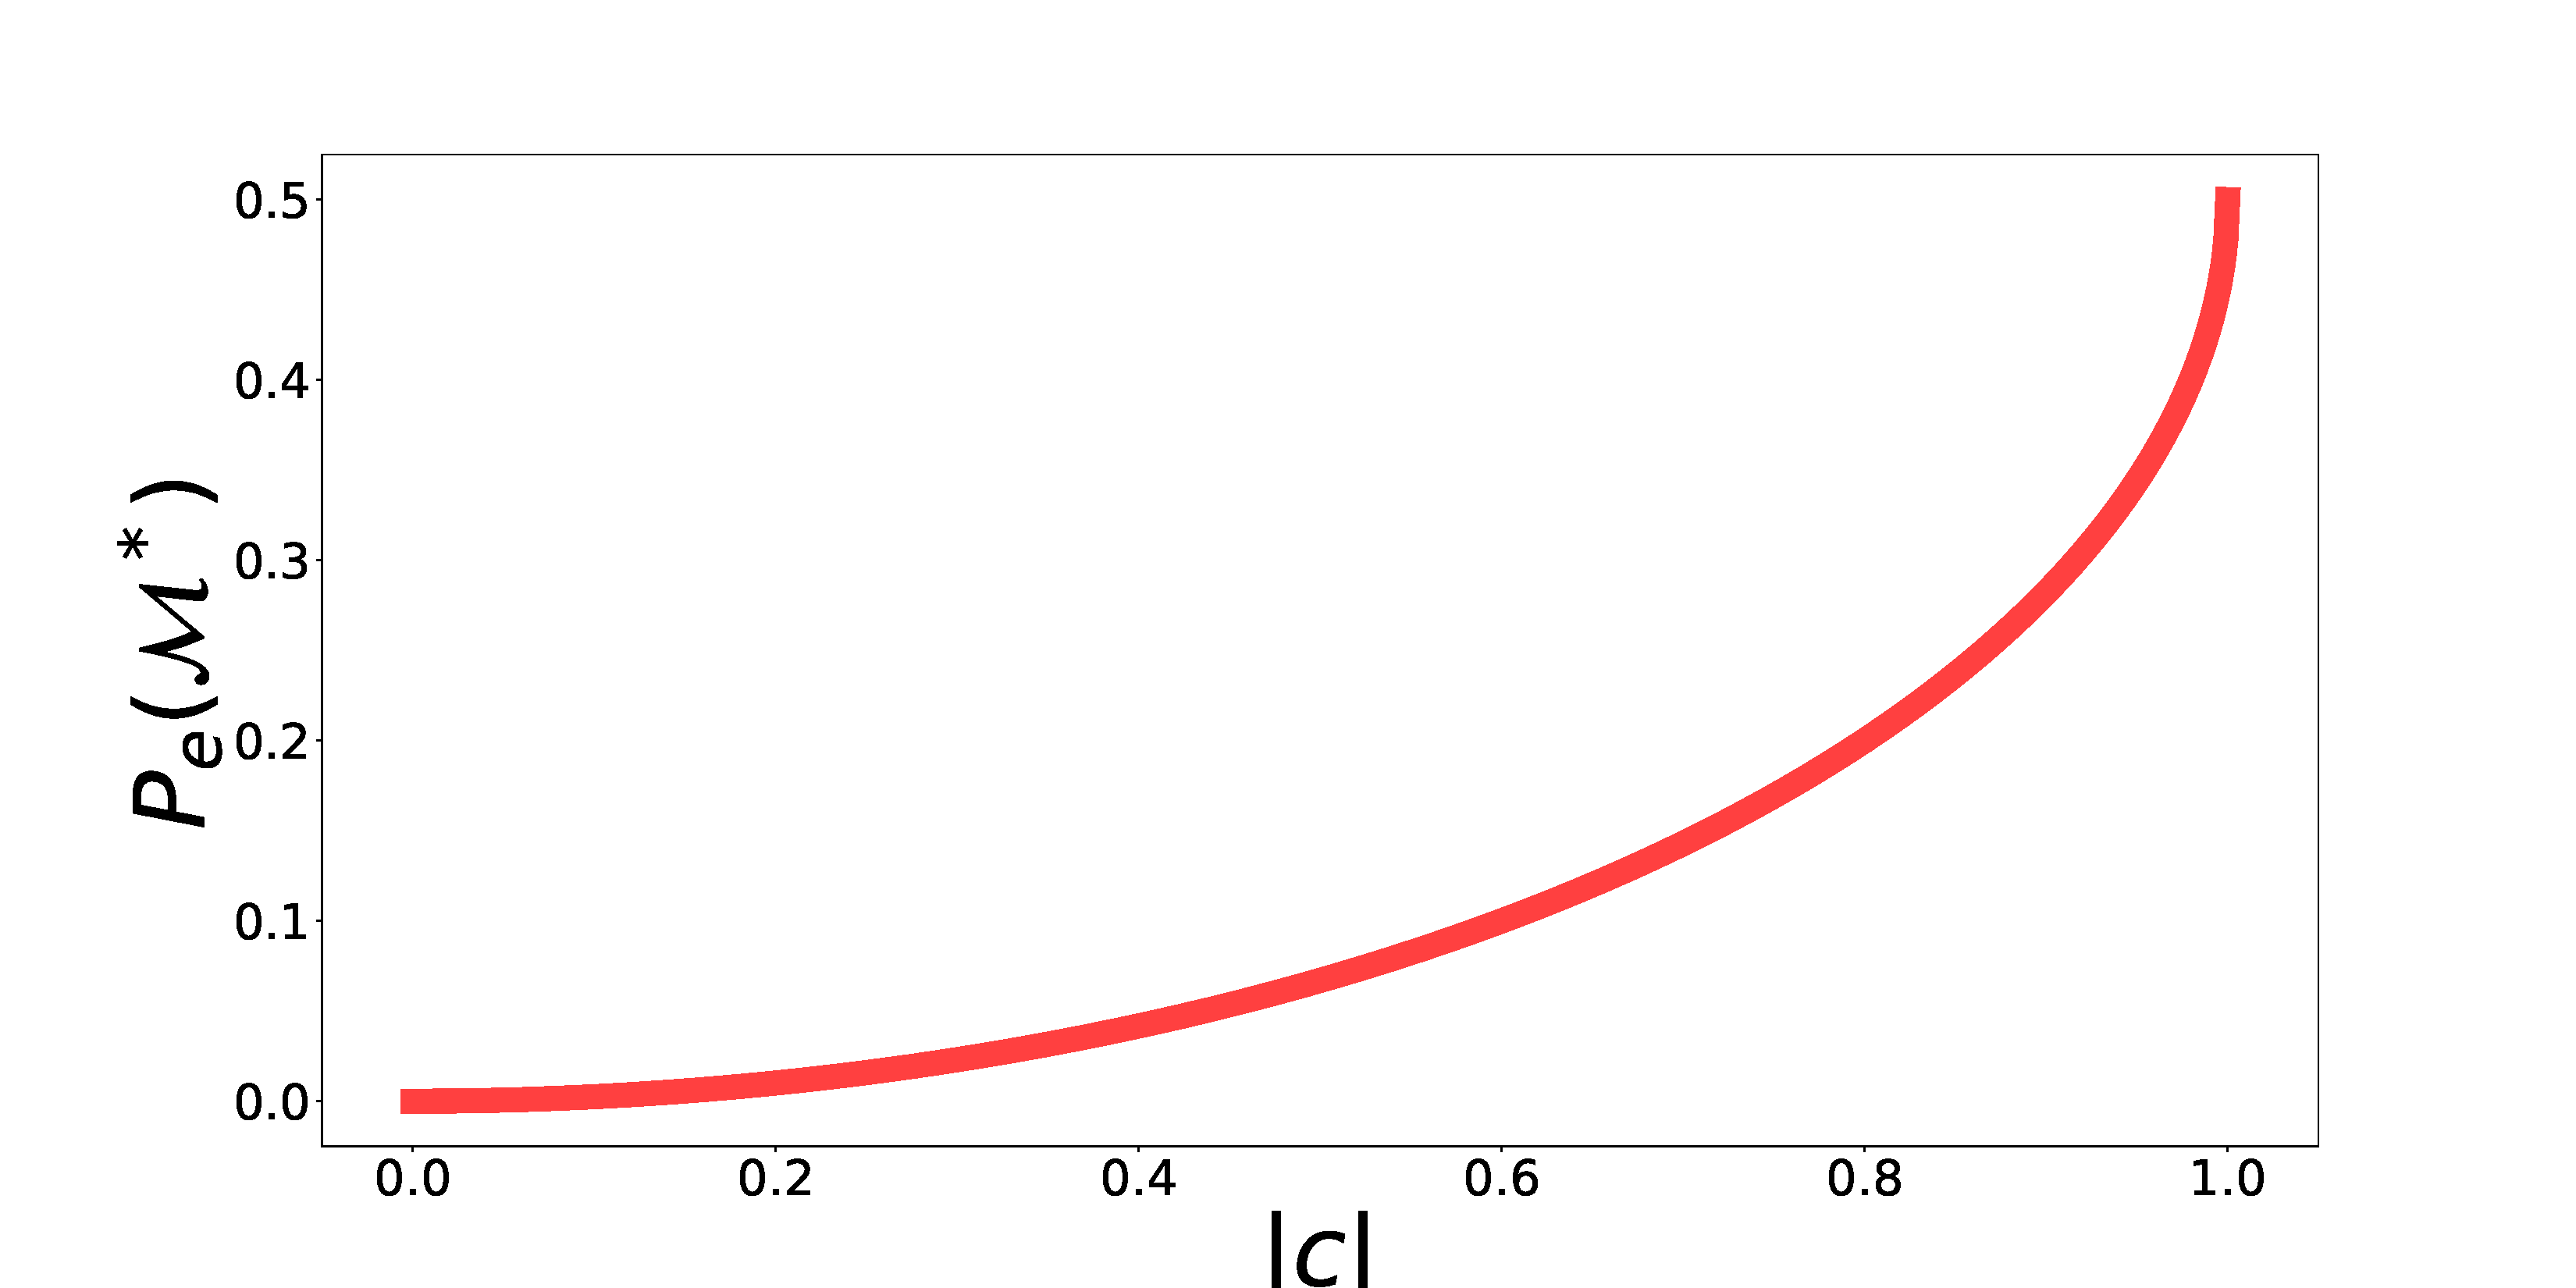
\includegraphics[width=1.\textwidth]{Figures/117/helstrom.pdf}
    \caption{We show Helstrom bound for the error probability when discriminating between two pure states as a function of their overlap $c$ (aboslute value).}
    \label{fig:helpure}
\end{figure}

To sum up, we have discussed the basics of single-shot quantum state discrimination; long is the road that continues this discussion. For instance, we ommited unambiguous state discrimination, where we demand that every time we guess for one hypothesis no errors are commited. This requires that we allow an extra \textit{I don't know outcome}, that deems that data inconclusive; in such case we are interested in minimizing the probability associated to such inconclusive outcome.

Also, we have not discussed multiple-hypothesis problems. In particular, closed-form solutions are known if the states are generated by a symmetry group; here, the optimal POVM is the \textit{pretty-good} (or square-root) measurement, and can be obtained explicitely in terms of the candidate states. In the non-symmetric case, such measurement often provides a \textit{pretty-good} success probability~\cite{Wooters1994prettygood, CrokeReviewQSD}. Also it is worth mentioning that semidefinite programming~\cite{boyd} will not be discussed here. The latter is a technique that allows to efficiently convex optimization problems (and relates to state discrimination when numerically optimizing over measurements).

%



% \subsubsection{Beyond minimum-error state discrimination}
% \textit{Unambiguous state discrimination} The POVM $\mathcal{M}$ can be constructed in such a way to allow for unambiguous discrimination, at the cost of potentially label outcomes as unconclusive. Here, $\mathcal{M} = \{ M_0, M_1, M_? \}$, and the unconclusive outcome is obtained with probability $p_?(\mathcal{M}) = \sum_{k=0,1} p_k p(?|k)$. For instance, in the case of pure states, we can readily construct the measurement operators as projectors onto orthogonal subpsaces of the states constituing the hypothesis; these are $M_0 = \frac{\proj{\psi_1^\perp}}{1+\braket{\psi_0}{\psi_1}}$ (guesses for $\ket{\psi_0}$),
% $M_1 = \frac{\proj{\psi_0^\perp}}{{1+\braket{\psi_0}{\psi_1}}}$
% (guesses for $\ket{\psi_1}$) and $M_? = \mathbb{I} - M_0 - M_1$ (leading to the unconclusive outcome); note that the accompanying coefficients of the projectors ensure that $M_? \geq 0$. We can readily see that when either outcome 0 or 1 are obtained, the test is conclusive, while a finite probability of unconcluding the test arises. In this setting, the challenge is thus to minimize the probability of undeciding, which is certainly relevant if no errors can be admitted in the discrimination task.
%
% \textit{Multiple-state discrimination $\&$ the Pretty Good Measurement}. We have seen that the optimal measurement in the minimum-error binary discirmination scenario is given by a complicated projection defined by the states to be distinguished. The optimal measurement in the multiple-hypothesis scenario has in general an unknown structure; nonetheless a \textit{pretty good measurement} (or square root measurement) can be derived, which in different scenarios such as symmetric pure states turns out to be optimal. Such approach constructs the optimal measurement from the square root of a mixture between the hypothesis states~\cite{Wooters1994prettygood, CrokeReviewQSD}.
%
% \textit{Semi-definite programming}. The optimization over POVM can be casted as a convex problem, which in turn can efficiently be solved through. Moreover, a dual problem can be formulated, which sometimes allows for analytical solutions (or bounds) useful for the problem at hand. For instance, it has been shown using this technique that the Dolinar-type receivers we consider in Chapter~\ref{chapter:RLCOH} can not be optimal when dealing with more than two hypothesis~\cite{Optimal2018Nakahira}.
%
% \textit{Beyond one-shot discrimination}. Discerning between quantum states is thus a primitive related to the description of physical entities. In its general setting, it is not possible to perfectly distinguish between two states, and either a finite probability of undecision arises, or one seeks for minimum-error strategies. In this thesis, we will focus on the latter. As shown above, the success probability is bounded in the one-shot scenario, but more information can certainly be acquired if more copies of the states are available. In turn, the error probability exponentially decreases with the number of copies, and deriving rates at which it does so is the matter of \textit{quantum hypothesis testing}. For example, in the \textit{i.i.d.} scenario, generalizations of the classical testing framework are known: while the symmetric error decrases with a rate known as the quantum Chernoff coeficient\cite{Audenaert2007Discrimination}, the assymmetric errors have quantum relative entropies as rates~\cite{Hiai1991,Stein2}. In these lines, the optimal measurement attaining such rates might be highly non-local (\textit{i.e.} act globally on all the copies available). Nevertheless, for the case of binary pure state discrimination, it has been shown that one can be assymptotically optimal if measuring locally and bayesian updating the priors~\cite{Acin2005Multi}.
%
% We will now review the framework of (classical) statistical inference, which will serve as a basis for characterizing quantum evolutions from measurement signals in Chapter~\ref{chapter:CMON}.
% \textit{A brief comment about quantum communications}
% What happens if we want to transmit a classical message over a quantum channel? such many information processing tasks depends on it. For instance, when capacity-attaining codes such as polar codes ~\cite{qpcodeswilde} rely on performing Helstrom measurement.


%%%


\subsection{Back to the classics: asymetric hypothesis testing}\label{ssec:asym}
Error probabilities non-trivially depends on the amount of data available, \textit{e.g.} the number of samples. Intuitively, the more data we have (\textit{e.g.} the more we have sampled our system), the smaller should the errors be on average. Quite generically, it can be seen that the error decays exponentially with the number of samples, with a rate that is an entropic function of the two underlying distributions; we will discuss some characterizations of such rates later in this Section.
%
% i.e. $\epsilon\sim e^{-r(\rho,\sigma) N}$, where the function $r(\rho,\sigma)$ depends on the precise setting (symmetric, asymmetric). In the independent and identically distributed (\textit{i.i.d}) scenario, much can be discussed about errors' behaviour, specially in the asymptotic limit of large number of samples.

In this context, a very powerful lemma known as the \textit{Neyman-Pearson lemma}, provides the statistic that is optimal for a wide range of settings.

\textit{Neyman-Pearson Lemma}. Given a binary hypothesis testing problem where we need to tell if data $\xf = (x_1,...,x_n)$ has been sampled from either $H=H_0$ or $H=H_1$, for $T>0$ we define the \textit{acceptange region} as
\equ{A(T)  = \Llaves{\frac{p(\xf|H_1)}{p(\xf|H_0)} \geq T},}
where $\xf$ are the samples acquired, and $T$ is the \textit{decision-boundary} (note that the point $T=1$ is where the hypothesis are equally likely). The decision region plays a prominent role in the values that the resulting errors take, and in this case read $\alpha^* = p \big(A(T)|H_0\big)$ and $\beta^* = p(\overbar{A(T)}|H_1)$\footnote{$\overbar{A(T)}$ denotes the complement of $A(T)$, \textit{e.g.} $\overbar{A(T)} = \Llaves{\xf: \frac{p(\xf|H_1)}{p(\xf|H_0)} <T}$}. Now, consider any other decision region $B$, whose error probabilities are $\alpha_B$ and $\beta_B$.
Then, the lemma states that if $\alpha_B \leq \alpha^*$, it follows that
$\beta_B \geq \beta^*$ (and also if $\beta_B \leq \beta^*$ then $\alpha_B \geq \alpha_*$)\footnote{The proof of the lemma is straightforward, and consists on exploting decision functions associated to $A(T)$ and $B$, and playing a bit with the definition of $A(T)$.}.

As discussed previously, we are generally interested in minimizing $\beta$ error when keeping $\alpha$ bounded. Considering the set of all possible statistics that can be defined, the power Neyman-Pearson lemma is that of providing the optimal one, which is given by the \textit{log-likelihood ratio}.

\subsubsection{Large deviations and assymptotic error rates}
The dependence of the error probabilities is non-trivial with repect to the number of samples available, and we intuitively expect that the error probabilities become smaller and smaller when more data is acquired. This is can be formally studied, and we here provided a short outline of the topic.

We will begin by discussing the notion of \textit{random variable concentration}. We consider the random sequence $\xf$ with $x_k \in \mathcal{A} = \llaves{a_1,...,a_M}$, and consisting on $n$ \textit{i.i.d} samples, whose underlying probability will be denoted by $Q$, \textit{i.e.} $Q^{n}(\mathbf{x}) = \prod_{k=1}^n Q(x_k)$

We define a \textit{type} $P_\mathbf{x}(\mathcal{A})$ ---for simplicity we will denote it as $P_\mathbf{x}$)--- which is the empirical probability distribution of each letter in alphabet $\mathcal{A}$, associated to the sequence $\mathbf{x}$, \textit{i.e.} $P_\mathbf{x}(a) = \frac{N_\mathbf{x}(a)}{n},\; \forall a \in \mathcal{A}$, where $N_\mathbf{x}(a)$ is the number of times that letter $a$ appears in $\xf$.
Next, we define as $\mathcal{P}_n$ as the set comprising all possible types $P$ generated by a denominator $n$. %\footnote{Note that the number of all such types is at most polynomial in $n$, \textit{i.e} $|\mathcal{P}_n|\leq (n+1)^{|\mathcal{A}|}$.}.
For example taking a binary alphabet $\mathcal{A} = \llaves{0,1}$, we get
\begin{equation*}
\mathcal{P}_n = \llaves{\big(P(0), P(1)\big): \Big(\frac{0}{n},\frac{n}{n} \Big), \Big(\frac{1}{n},\frac{n-1}{n}\Big) ... ,\Big(\frac{n}{n}, \frac{0}{n}\Big)}.
\end{equation*}
Since many sequences can lead to the same type, we define the type class $T(P)$ as
\equ{T(P) = \llaves{\mathbf{x}: P_\mathbf{x} = P}.}
Now, the probability of a given sequence $\mathbf{x}$, which is $i.i.d.$ and sampled from $Q$ can be written in terms of its type $P_\mathbf{x}$ as\footnote{To see this, we expand the total probability of $\mathbf{x}$ and exploit the $i.i.d.$ property:
\begin{align*}
Q(\mathbf{x}) = \prod_k Q(x_k) =\prod_{a\in\mathcal{A}}Q(a)^{N_\mathbf{x}(a)} &= \prod_{a\in \mathcal{A}}Q(a)^{n P_\mathbf{x}(a)} \\
&= e^{-n \Big(\sum_{a\in\mathcal{A}} P_\mathbf{x}(a) \log{\frac{P_\mathbf{x}(a)}{Q(a)} - P_\mathbf{x}(a) \log{P_\mathbf{x}(a)}}\Big)},
\end{align*}
where the last terms in the exponent can is the relative entropy and Shannon entropy respectively.}
\eq{probSEQ}{Q(\mathbf{x}) = e^{-n\Big(D(P_\mathbf{x} || Q) + H(P_\mathbf{x})\Big)},}
where the relative entropy between two (discrete) random-variable distributions is defined as $D(p||q)=\sum_k p_k \log{\frac{p_k}{q_k}}$ and $H$ is the Shannon entropy.% $H(p) = -\sum_k p_k \log{p_k}$.

From Eq.~\ref{eq:probSEQ} we can readily see that for typical sequences, i.e. sequences
$\mathbf{x}$ with  $P_\mathbf{x}=Q$, $Q(\mathbf{x}) = e^{-n H(Q)}$, i.e. its occurrence is given by the entropy of $Q$.

It can be shown that the size of a given type class (that is the number of sequences with a given empirical distribution) is asymptotically given by $|T(P)|\sim e^{n H(P)}$. This allows us to write the probability of a given type class as
\equ{Q\Big(T(P)\Big)=|T(P)|e^{-n\Big(D(P_\mathbf{x}=P || Q) + H(P)\Big)} \sim e^{-n D(P||Q).}}

This shows that type class corresponding to the typical distribution is exponentially most probable that any other type. This puts on solid grounds that if one samples a distribution many times the frequency of symbols  will be essentially equal to the probabilities. $\frac{N(a)}{n}=Q(a)$ with high probability.

For example, considering again the tossing-coin example, with a heads probability of $q$. For $n$ samples the types $\mathcal{P}_n$ can be fully characterized by the number of heads, \textit{i.e.} $\mathcal{P}_n = \llaves{\Big(\frac{k}{n}, \frac{n-k}{n}\Big)}_{k=1}^n$, and the random variables concentrate around the type $k$ given by $\frac{k}{n} = q$ as $n\to\infty$.

\vspace{1cm}
Let us return to the likelihood ratio, which given a random sequence $\mathbf{x}$ is obtained as $\Lambda(\mathbf{x})=\frac{p_1(\mathbf{x})}{p_0(\mathbf{x})}$. In the \textit{i.i.d.} setting we can link the logarithm of the likelihood ratio, which we call the \textit{log-likelihood ratio} and denote by $\ell$, to the relative entropies as
\begin{align}\label{eq:loglikiid}
\ell(\xf) = \log{\frac{p_1(\xf)}{p_0(\xf)}} &= \sum_{i=1}^n \log{\frac{p_1(x_i)}{p_0(x_i)}} \\ &= \sum_{a\in\cA} n P_\xf(a) \log{\frac{p_1(a)}{p_0(a)}} \\ \nonumber
&= \sum_{a\in\cA} n P_\xf(a) \log{\frac{p_\xf(a)}{p_0(x_i)} - \sum_{a\in\cA} n P_\xf(a) \log{\frac{p_\xf(a)}{p_1(x_i)}}} \\ \nonumber
&= n \Big[ D(P_\xf||p_0) - D(P_\xf||p_1) \Big] \nonumber.
\end{align}

From here it is immediate to see that the expectation value of log-likelihood under hypothesis
$H_1$ is given by the relative entropy, $\expect{\ell}_{1}/n=D(P_1||P_0)$, and under $H_{0}$
 by $\expect{\ell}_{0}/n=- D(P_0||P_1)$. Moreover, from our previous discussion on the theory of types, it also follows that $\ell/n$ concentrates around these values:
 \eq{concenELL}{\frac{\ell(\xf)}{n} \underset{n\rightarrow\infty}{\longrightarrow} D(P_1||P_0).}
under $H_{1}$ (and similarly with $H_0$).

Neyman-Pearson's Lemma in conjunction with the theory of types also allows us to easily asses the asymptotic error rates for  \textit{i.i.d.} sampling. It is clear that the decision region depends only on the type class of the observed sequence (in the case of the coin, the total number of head and tails).

Then, for symmetric hypothesis testing, the optimal decision region corresponds to guessing for the most probable hypothesis (given the observed empirical distribution) or equivalently guessing hypothesis
$H_{1}$ ($H_{0}$) if $\ell>0$ ($\ell\leq 0$). It is easy to check that the error rate for $P_{err}^{(n)} = \pi_0 \alpha_n + \pi_1 \beta_n$ is dominated by the events were $\ell=0$, i.e. $D(P_\xf||p_0) - D(P_\xf||p_1) =0$.
That is, we obtain the \textit{Chernoff coefficient}:
\eq{chernoff}{C^*=\underset{n\rightarrow\infty}{\text{lim}} - \frac{1}{n}\log{\underset{A_n}{\text{ min }} P^{(n)}_{err}},}
where $C^* = D(P_{\lambda^*}||P_1) = D(P_{\lambda^*}||P_0)$, meaning that $\lambda^*$ is determined by the probability distribution $P_\lambda$ for which the relative entropy to $P_0$ equals the relative entropy to $P_1$\footnote{Such probability distrbution has the structure $P_\lambda(x) = \frac{P_0^{\lambda}(x) P_1^{1-\lambda}(x)}{\sum_{a\in\cA} P_0^\lambda(a)P_1^{1-\lambda}(a)}$, which leads to an alternative (and more common) expression for $C^* = -\underset{0\leq\lambda\leq 1}{\text{ min }} \log{\sum_{a\in\cA} P_0(a)^\lambda P_1^{1-\lambda}(a)}$
}.

Similarly, in the asymmetric setting one can get the largest error exponent (fastest decay of the error), while keeping a finite probability for the other type error (recall that we wish to diagnose correctly at least a fraction of the healthy patients). This is is formalized in the following lemma.

\textit{Stein-lemma}. Let $\xf$ be a sequence of \textit{i.i.d.} samples obtained from $Q$. We consider an hypothesis testing scenario where the models are given by $Q=P_1$ and $Q=P_0$. Let $A_n$ be an acceptance region for hypothesis $H_1$, and the error probabilities be $\alpha_n = P(\bar{A}_n|H_0)$ and $\beta_n = P(A_n|H_1)$. Let $0<\epsilon<\frac{1}{2}$, and define $\beta_n^\epsilon = \underset{A_n}{\text{min}}\;\beta_n$ such that $\alpha_n<\epsilon$.
Then the optimal error exponent is
\eq{stein}{ -\underset{n\rightarrow\infty}{\text{lim}} \frac{\log{\beta_n^\epsilon}}{n} = D(P_0||P_1).}

Note that this rate is independent of the particular value of $\epsilon$. Similarly, the $\alpha$ error is minimized instead (while keeping $\beta<1/2$, then the optimal rate is given by $D(P_1||P_0)$.
The relative entropies appearing in the Stein lemma, are strictly larger than the Chernoff coefficient, as it should since in the symmetric scenario both (optimal) errors must decay exponentially, whereas in the asymmetric case only one them remains constant.

Finally, note that the error rates provide an operational interpretation to the relative entropy and the Chernoff coefficient as measures of distinguishability between the two probability distributions.

\subsubsection{Quantum hypothesis testing: a brief comment}
While we provided an introduction to the classical hypothesis testing problem, and this suffices for the scope of this thesis, we will here outline how this situation generalizes to the quantum realm. Contrary to the single-shot quantum-state discrimination scenario, we are here given $N$ copies of the same quantum state, and it is desired to identify its nature among two (or more) alternatives. In this case, since more information is available, our performance is expected to be better on average, similarly to the results discussed in Sec.~\ref{ssec:asym}. The scope of possible strategies is, however, non-trivially larger. In turn, we can choose to perform either a separable quantum measurement (individually measure each copy), an adaptive quantum measurement (where the result of the previous copy conditions the next quantum measurement to be performed), or a joint measurement acting on all the $N$ copies at once, or even any combination of the above strategies. In this context, a quantum version of the Neyman-Pearson lemma discussed above can be formulated:

\textit{Quantum Neyman-Pearson Lemma}
Given a binary hypothesis testing problem with the two hypotheses:  $\rho$ ($H_{1}$) vs. $\sigma$ ($H_{0}$). For  $T>0$ define a two outcome POVM $M=\{M_{0},M_{1}=\mathbb{I} -M_{0}\}$ with
\begin{equation}\label{eq:optalphabeta}
M_{1}(T)=\mathbb{I} _{(\rho-T \sigma)>0}
\end{equation}
where $\mathbb{I} _{\Delta>0}$ is the projector on the positive part of $\Delta$,
and the corresponding error probabilities $\alpha^{*}=P(M_{1}|H_{0})=\tr{M_{1}(T)\sigma}$ and $\beta^{*}=P(M_{0}|H_{1})=\tr{M_{0}(T)\rho}$. Given any measurement $F=\{F_{0},F_{1}\}$ and its associated error probabilities $\alpha_{F}$ and $\beta_{F}$. If $\alpha_{F}\leq\alpha^{*}$ then $\beta_{F}\geq \beta^{*}$(and vice versa).

The projective measurement $M_{1}(T)$ is the quantum analog of the likelihood test which defined the acceptance region (for hypothesis $H_{1}$)
$$A=\left\{ \mathbf{x}: \frac{P_{1}(\mathbf{x})}{P_{0}(\mathbf{x})}> T\right\}=
\left\{ \mathbf{x}: P_{1}(\mathbf{x})-T P_{0}(\mathbf{x})> 0 \right\}$$
Note also from \eqref{eq:optalphabeta} that such class of measurements $M_{1}(T)$ is optimal when one wishes to minimize the linear combination of errors  $\alpha^{*}+T  \beta^{*}$, \textit{e.g.} in symmetric hypothesis testing taking the parameter $T$ to be the ratio of priors: $T=\pi_{0}/\pi_{1}$. For this case the Helstrom bound from last section is recovered.

Generally, the optimal error probability decreases exponentially with the number of copies, and deriving rates at which it does so is the matter of \textit{quantum hypothesis testing}. For example, in the \textit{i.i.d.} scenario, generalizations of the classical testing framework are known: while the symmetric error decrases with a rate known as the \textit{quantum Chernoff coeficient}\cite{Audenaert2007Discrimination}, the asymmetric errors have quantum relative entropies as rates~\cite{Hiai1991,Stein2}. Strikingly, such rates are often obtained by replacing the classical expression of the entropic functions with the quantum one. The optimal measurement attaining such rates might be a global one (\textit{i.e.} acting jointly on all the available copies). We remark, however, that for the case of binary pure state discrimination, it has been shown that one can be assymptotically optimal when measuring locally and updating the priors in a Bayesian manner~\cite{Acin2005Multi}, a result that turns useful when proving the optimality of Dolinar's receiver in Sec.~\ref{ssec:tdol}. Furthermore, the setting of quantum sequential hypothesis testing has recently been formalized and studied in Ref.~\cite{Vargas2021quantum}, and we will now turn to study the classical version of it.

\subsection{Sequetial hypothesis testing}\label{ssec:sprt}
So far we have discussed the hypothesis testing setting in which $n$ samples of data where presented to us, and a decision needs to be made for the underlying hypothesis. We introduced different figures of merits, taking into account the importance given to each error type. Following, we introduced the log-likelihood ratio, which via the Neymann-Pearson lemma turns out to be the optimal statistic. Then, we have discussed the assymptotic behaviour of the errors, which in the \textit{i.i.d.} are exponentially decaying, with a rate given by either the relative entropy (assymetric scenario) or the Chernoff coefficient (symmetric scenario).

Strikingly, by slightly relaxing the setting, more efficient strategies can be brought to the stage. This consists in relaxing the condition that the underlying hypothesis needs to be determined after observing the random sequence $\xf$ (of length $n$). Instead, we could think of allowing for an extra label that deems $\xf$ as unconclusive. In this case, further samples will be required, and the test proceeds in a \textit{sequential} fashion until a given criterium is met.

Thus, a sequential strategy is characterized by \textit{(i)} \textit{a stopping rule}, that tells whether to stop the sampling process or to demand an additional sample, and \textit{(ii)} \textit{a decision rule} which selects one hypothesis or the other in case of stopping the test. Moreover, we will consider an scenario in which one can guarantee that \textit{for each realization of the test}, the conditional probability of correctly identifying each of the hypothesis is above some pre-defined threshold. This is known as a \textit{strong errors guarantee}, \textit{i.e.} given $\epsilon_k$ ($k=0,1$), the test assures that
\eq{strongSPRT}{p(H_k|\xf_n)\geq1-\epsilon_k.}
These conditions cannot always be achieved by a test with a fixed-horizon --- since there is a chance that the random sequence is not informative enough to assert the correctness of Eq.~\ref{eq:strongSPRT} for \textit{both} hypothesis ---. On the contrary, if new samples are required until conditions in Eq.~\ref{eq:strongSPRT} are fullfiled, then we can readily devise a test --- known as the Sequential Probability Ratio Test (SPRT)~\cite{Wald1948Optimum} --- that consists on the following. Starting at $n=1$, at each step $n$ check if
\begin{enumerate}
\item $p(H_1|\xf_n) \geq 1-\epsilon_1$. If this happens, \textit{stop} and accept $H_1$, with a success probability guaranteed to be $P_{s_1} = 1-\epsilon_1$.
\item $p(H_0|\xf_n) \geq 1-\epsilon_0$. If this happens, \textit{stop} and accept $H_0$, with a success probability guaranteed to be $P_{s_1} = 1-\epsilon_0$.
\item If neither of 1. nor 2. is acccomplished, then continue sampling and move to the next step.
\end{enumerate}
This procedure can be casted in terms of the log-likelihood ratio $\ell_n = \ell(\xf_n)$ at step $n$. By using Bayes theorem, we can readily construct an \textit{undecision} region $\Omega = [a_0, a_1]$ such that
\begin{align}\label{eq:decisionsASPRT}
a_1 &= \log{ \Big(\frac{1-\epsilon_1}{\epsilon_1} \frac{p_0}{p_1} \Big)}\\
a_0 &= \log{\Big(\frac{\epsilon_0}{1-\epsilon_0}\frac{p_0}{p_1} \Big)}\nonumber
\end{align}
and then the test proceeds at step $n$ as follows:
\begin{itemize}
\item Compute the log-likelihood ratio $\ell_n$
\item If $\ell_n \geq a_1$ \textit{stop} the test, and accept $H_1$, with a success probability guaranteed to be $P_{s_1} = 1-\epsilon_1$
\item Alternatively, if $\ell_n \leq a_0$, \textit{stop} the test, and accept $H_0$, with a success probability guaranteed to be $P_{s_0} = 1-\epsilon_0$
\item On the contrary, if $\ell_n \in \Omega$, demand an extra sample and repeat the test for step $n+1$.
\end{itemize}

As explicited by Eq.~\ref{eq:loglikiid}, in the \textit{i.i.d.} scenario the log-likelihood ratio can be casted as a sum of contributions $\ell_k = \ell(x_k)$ that are sequentially-acquired:
\eq{logsumrandom}{\ell(\xf_n) = \log{\frac{p(\xf|H_1)}{p(\xf|H_0)}}) = \sum_{k=1}^n \ell_k, \spacee \ell_k = \log{\frac{p(x_k|H_1)}{p(x_k|H_0)}}.}
The beauty of this relies on \textit{the random walk interpretation}: with each new sample, a step of length $\ell_k$ is taken with probability $p(\xf_k|Q)$, where $Q$ is the underlying probability distribution, \textit{i.e.} either $P_0$ or $P_1$. From here, we can readily see that the walker will have a positive (negative) drift when $H_1(H_0)$ is the underlying hypothesis: by denoting the log-likelihood ratio obtained under hypothesis $i$ as $\ell_{|i}$, we have
\begin{align}
\expect{\ell(\xf_n)}_{|1} &= n D(P_1||P_0) \\ \nonumber
\expect{\ell(\xf_n)}_{|0} &= -n D(P_0||P_1).
\end{align}
These drifts values indicate that the random walk will likely hit the decision boundary that corresponds to the underlying hypothesis, since it moves with an average speed given by the relative entropy. However, it might well be that the stochastic nature of the process leads the walker to hit the complementary decision boundary. Either the case, Wald proved that the walker eventually exits the undecision region $\Omega$, and thus the process stops~\cite{Wald1948Optimum}. The time ---or sample number--- at which the process stops is known as \textit{the stopping time}, and we denote it by $\tau$:
\eq{stop_time}{\tau := \underset{n}{\text{inf}}\llaves{n:\ell(\xf_n)\notin\Omega}.} Thus, the stopping time refers to the first instance at which the process leaves the $\Omega$ region, and we have that the probability of the walker to be inside the region $\Omega$ goes to zero as the number of samples goes to infinity. In the following, we will intercheangably refer to $\tau$ as the number of samples $n$ at which the process stops, since this Section will serve as a reference for the continuous-time processes analyzed in Chapter~\ref{chapter:CMON}.

The average position of the walker at step $\tau$, \textit{e.g.} the value of $\expect{\ell(\xf_\tau)}$ can be linked to the average value of the stopping-time $\tau$ via the Wald's identity~\cite{probcompbook}:
\eq{waldIdentity}{\expect{\ell_(\xf_\tau)}_{|i} = \langle\sum_{k=1}^\tau \ell_k \rangle_{|i} = \expect{\ell_k}_{|i},}
resulting in
\begin{align}\label{eq:waldsolved}
\expect{\tau}_{1} &= \frac{\expect{\ell}_{1}}{D(P_1||P_0)}, \\
\expect{\tau}_{0} &= -\frac{\expect{\ell}_{0}}{D(P_1||P_0)}.
\end{align}

Thus, it becomes clear that the value of the log-likelihood at the stopping time (the moment when it exits the undecision region) will be essentially given its value at the boundary (essentially $a_{0}$ or $a_{1}$ for hypothesis $H_{1}$ or $H_{0}$, respectively). Hence, as we will show more rigorously below,
\begin{align}\label{eq:waldsolved}
\expect{\tau}_{1} &\sim \frac{a_{1}}{D(P_1||P_0)}, \\
\expect{\tau}_{0} &\sim -\frac{a_{0}}{D(P_1||P_0)}.
\end{align}

The last equation clearly shows that the average value of the likelihood ratio is proportional to the average-time required to reach the corresponding decision boundary, and the slope is given by the relative entropy between the probability distributions under consideration. Since the relative entropy is generally not symmetric, \textit{i.e.} $D(P_0||P_1)\neq D(P_1||P_0)$, we expect the average stopping-times to differ when swapping the underlying model. Thus, it is interesting to ask how many samples would be required, on average, to stop the process; this will in turn depend on the quality of the sequential test, as given by the strong error conditions of Eq.~\ref{eq:strongSPRT}.

Let us see now how does SPRT perform regarding the type-I and type-II errors, in particular in the regime where $|a_{i}|$ asymptotically large (small errors), where  $\text{Pr}\big[\ell(\xf_n) \in \Omega\big] \underset{n\rightarrow\infty}{\longrightarrow}0$ holds. For simplicity, we define
\begin{align*}
A = e^{a_1} = \frac{1-\epsilon_1}{\epsilon_1} \frac{p_0}{p_1}, \quad B =e^{a_0} =  \frac{\epsilon_0}{1-\epsilon_0} \frac{p_0}{p_1}.
\end{align*}
Then, the weak errors can be linked to the decision thresholds as follows
\begin{align}
\alpha &= p(\hat{H}_1|H_0) = \sum_{\xf \in \mathbf{\mathcal{X}}_0} p(\xf|H_0) \leq A^{-1}  \sum_{\xf \in \mathbf{\mathcal{X}}_0} p(\xf|H_0) = A^{-1}(1-\beta)\\
\beta &= p(\hat{H}_0|H_1) = \sum_{\xf \in \mathbf{\mathcal{X}}_1} p(\xf|H_1)\leq B \sum_{\xf \in \mathbf{\mathcal{X}}_1} p(\xf|H_0) = B (1-\alpha),
\end{align}
where used that, when stopping the test, the log-likelihood ratio is either higher (smaller) than $a_1(a_0)$, and defined the decision regions $\mathbf{\mathcal{X}}_k$ under which the test decides for the $k^\text{th}$ hytpothesis.

Moreover, the inequalities above saturate if there is no \emph{overshooting}, that is if the
process stops exactly at the boundary. This happens either approximately when the step-sizes $\ell_{k}$ are small relative to $a_{i}$, as mentioned above, or if the log-likelihood evolves continuously --- \textit{e.g.} if we are sampling from a Wiener-like process, as discussed in Sec.~\ref{ssec:ito}, and analyzed in Chapter~\ref{chapter:CMON}. In that case the above relations can be inverted to get

\begin{align}\label{eq:weakErrorsSPRT}
\alpha &= \frac{1-B}{A-B} = \frac{1-e^{a_0}}{e^{a_1}-e^{a_0}} = \frac{\epsilon_1(p_1 -\epsilon_0)}{p_0(1-\epsilon_0 -\epsilon_1)}\\
\beta &= \frac{B(A-1)}{A-B} =  e^{a_0}\frac{e^{a_1}-1}{e^{a_1}-e^{a_0}} = \frac{\epsilon_0 (p_0 - \epsilon_1)}{(1-\epsilon_0-\epsilon_1)p_1}.
\end{align}

Thus, imposing strong-error conditions fixes the value of the weak errors in the SPRT. Note that in the case that the boundaries are very large in absolute value, \textit{e.g.} $a_0 \rightarrow -\infty$ and $a_1 \rightarrow\infty$, corresponding to very small values of $\epsilon_0$ and $\epsilon_1$ respectively, then
\begin{equation}\label{eq:largeBoundaries}
\alpha \sim e^{a_0}\sim \epsilon_1, \quad \beta \sim e^{-a_1}\sim \epsilon_0.
\end{equation}

\textit{$\ell(\xf_\tau)$ as binary random-variable}. In the non-overshooting case, the log-likelihood ratio $\ell(\xf_\tau)$ can take two values once the SPRT stops, which are determined by the region $\Omega$, \textit{e.g.} $\ell(\xf_\tau)\in\llaves{a_0,a_1}$. For instance, if the underlying probability distribution is $P_1$, then the walker will arrive to position $a_1$ with probability $p(\hat{H}_1|H_1) = 1-\alpha$, and otherwise arrive to position $a_0$ with probability $p(\hat{H}_0|H_1) = \beta$ (a similar reasoning applies when the underlying model is $P_0$), and thus we have that the mean-value of the $\ell(\xf_\tau)$ reads
\eq{mean_ell_binarySPRT}{\expect{\ell(\xf_\tau)}_{|_1} = a_1(1-\beta) + a_0 \beta, \quad \expect{\ell(\xf_\tau)}_{|_0} = a_0 \alpha + a_1(1-\alpha).}

From here, we can infer the number of samples required to stop the test, given pre-defined strong error thresholds. In turn, from Eq.~\ref{eq:mean_ell_binarySPRT}, the Wald identity in Eq.~\ref{eq:waldIdentity}, and the expressions of the weak errors in terms of the strong ones, one can readily identify the average stopping-time, whose expression is assymptotically given by
\begin{equation}\label{eq:sptrWaldsimple}
\expect{\tau}_{1} \sim -\frac{ \log{\epsilon_1}}{D(P_0||P_1)}, \quad \expect{\tau}_{0} \sim -\frac{\log{\epsilon_0}}{D(P_1||P_0)}
\end{equation}

Remarkably, the SPRT is \textit{optimal} regarding such resource~\cite{Wald1948Optimum}. This means that, for a pre-defined value of the weak errors $\alpha$ and $\beta$\footnote{To avoid confusion, recall that such errors are, in the SPRT, are fixed by the values of $\epsilon_0$ and $\epsilon_1$.}, the number of samples ---$\expect{\tau}_{|1}$ and $\expect{\tau}_{|0}$--- that a test would require to gather cannot be less than that of the SPRT, when accomplishing to such errors.

In this regard, the SPRT comes with a \textit{bonus}: not we one can attain the desired error rates faster, but also it is possible to certify the error commited for any given trajectory. This is in contrast to the approach presented in Sec.~\ref{ssec:asym}, which contrasts the hypothesis in a \textit{static} way. As expected, allowing the test to stop when enough evidence is gathered, results in a lower average number of samples; and when compared with its \textit{deterministic} counterpart, one can attain better error rates using the same resources (on average). Similarly, these results hold for the symmetric error probability in Eq.~\ref{eq:1_statinf_symm_ps}, \textit{e.g.} when the value $P_e = p_0 \alpha + p_1 \beta$ is fixed in advance, and a sequential test is carried out in order to optimize the average stopping time required to reach such error threshold~\cite{Gordon1976Improved}.

Thus, we will deem the test presented in Sec.~\ref{ssec:asym} --- which does not process the data sequentially but rather makes a decision once a fixed and pre-defined time-horizon has been reached--- as the \textit{deterministic} test. In Chapter~\ref{chapter:CMON} we will thoroughly study the performance of sequential tests in continuously-monitored systems and compare their performance with to respect to that of deterministic ones (those that gather data during a pre-established and fixed time).

\subsection{Parameter estimation}\label{ssec:1_stinf_estimation}
In this Section we discuss parameter estimation, and in particular the limits that (classical) information theory imposes to the accuraccy that can be attained when estimating a parameter encoded in a probability distribution function out of a finite number of samples.

Let $f(x, \theta)$ be a probability distribution function, parametrized by $\theta$ (as an example, a normal distribution $\mathcal{N}(\mu,\sigma)$ has parameters $\mu$ and $\sigma$). We interpret such object as being the probability of a sample to take the value $x$, given a known value of $\theta$. For instance, if $f$ has a strong dependence \textit{w.r.t.} $\theta$, we expect it to be easier to infer information about $\theta$, and fewer samples will be sufficient to estimate the value of the parameter with a given precision. On the contrary, if the landscape of $f$ looks flatter when varying the value of $\theta$, then we will require more samples to be sure that value of $\theta$ is the right one. This notion is captured by the \textit{score} of $f$:
\equ{s(x,\theta):=\partial_\theta \log{f(x,\theta)},}
whose mean value vanishes:
\begin{align*}
\mathbb{E}[s(x,\theta)] = \int_\mathbb{R} dx \partial_\theta \log f(x,\theta) f(x,\theta) = \partial_\theta \int_R dx f(x,\theta) = 0.
\end{align*}
where the last equality follows from the normalization $\int_R dx f(x,\theta)=1$. However, its variance contains information about the parameter-landscape, and reads
\begin{align*}
I(\theta):= \text{Var}[s] = \mathbb{E}_x[\big(\partial_\theta \log f(x,\theta)\big)^2] &= \int_\mathbb{R} dx f(x,\theta) \big(\partial_\theta \log f(x,\theta)\big)^2 \\&= \int_\mathbb{R} dx f(x,\theta) \Big(\frac{\partial_\theta f}{f}\Big)^2.
\end{align*}
The variance of the score is known as the \textit{Fisher information}, and we can explicitely see that is linked to the curvature of $f$ as per
\begin{align*}
\langle\partial^2_\theta \log f \rangle = \langle - \frac{(\partial_\theta f)^2}{f^2}\rangle + \cancelto{0}{\langle \frac{\partial^2_\theta f}{f} \rangle}.
\end{align*}
Overall, the Fisher information describes how the landscape of $f$ looks when varying the parameters $\theta$, and the following relation holds
\begin{align}I(\theta) = \mathbb{E}[(\partial_\theta \log f)^2] = - \mathbb{E}[\partial^2_\theta \log f].\end{align}
However, we are interested in providing an estimation of the parameter, given that we acquired a random (\textit{i.i.d}) sequence sampled from $f$. To this end we define an \textit{estimator} $\hat{\theta}$ to be an statistic that provides such value $\hat{\theta}$. For instance, the sample average $\expect{\bm{x}} = \frac{1}{n}\sum_k x_k$ is an (unbiased) estimator for the mean of $f$.

Among all possible estimators, we will find it useful to consider the \textit{maximum-likelihood} one, defined as
\equ{\hat{\theta} = \underset{\theta}{\text{argmax\;}} \log{f(\bm{x}, \theta)},}
where we note that since $\bm{x}$ consists on \textit{i.i.d.} samples, we can factorize the logarithm of the likelihood function as a sum of contributions, similarly to Eq.~\ref{eq:logsumrandom}. While the maximum-likelihood estimator is \textit{consistent}, in the sense that for a very large number of samples such estimator converges to the correct value almost surely, it might be \textit{biased} (in the sense that its expected value might differ from underlying true parameter we want to estimate)\footnote{Note however that any consistent estimator is assymptotically unbiased.}. This is in line with the fact that such estimator retrieves the parameter value which is most consistent with the observed data, but not with the average.

To end this discussion on parameter estimation, let us comment on a fundamental result that relates the ultimate performance of an estimator with the Fisher information. In turn, the \textit{Cramer-Rao bound} provides a lower bound to the variance of any (unbiased) estimator. This means that our confidence in the estimation cannot be higher than the information carried out by the underlying probability distribution function $f$, as given by the Fisher Information $I(\theta)$ introduced above. To see this, we consider an (unbiased) estimator of $\theta$, \textit{i.e} $\hat{\theta}$. If it is unbiased, then the following chain of equailities holds:
\begin{align*}
0 = \int dx f(x) \big(\hat{\theta}-\theta ) = \partial_\theta \Big[ \int dx f(x) \big(\hat{\theta}-\theta ) \Big] = -1 + \int dx \big(\partial_\theta f(x)\big)\; \big(\hat{\theta}-\theta ),
\end{align*}
and thus we conclude that $\int dx f(x) \big(\partial_\theta \log{f}\big) \big(\hat{\theta}-\theta) = 1$
If we now we use the Cauchy-Schwartz inequality, \textit{i.e.} $(u,v)^2 \leq (u,u) (v,v)$, we get
\begin{align*}
1^2 &= \Big[\int dx \Big((\hat{\theta}-\theta) \sqrt{f} \Big) \Big( \sqrt{f} \partial_\theta \log f(x) \Big) \Big]^2\\
&\leq \int dx \Big((\hat{\theta}-\theta) \sqrt{f} \Big)^2 \Big] \Big[ \int dx \Big( \sqrt{f} \partial_\theta \log f(x) \Big)^2 \\
&=  \text{Var}[\hat{\theta}] I(\theta).
\end{align*}

Thus, the Fisher information provides an ultimate (classical) bound for the variance of \textit{any} estimator. Note that in the case of $n$ trials the Fisher information, in the \textit{i.i.d.} case, is additive: $I_n(\theta) = n I(\theta)$, which can be seen from  $\mathbb{E} \partial_\theta^2 \log p(x)^n$.
Moreover, it can also be shown that in this limit the bound can be saturated (by a proper estimator, for instance, maximum-likelihood), and hence $\text{Var}[\hat{\theta}]\sim \tfrac{1}{n I(\theta)}$, a situation known as \textit{shot-noise limit}.

To conclude, we note that similar to hypothesis testing, the problem of parameter estimation gets a twist in the quantum realm, where again a non-trivial optimization over measurements (and probes) is involved. Moreover, a new object known as the \textit{quantum Fisher information} appears in the stage, accompanied by a \textit{quantum Cramer-Rao bound}. We will not discuss this topic, but refer the interested reader to Refs.~\cite{Meyer2021fisherinformationin,helstromBOOK,giovanetti2006quatnum}.


\section{Reinforcement learning}\label{sec:1_rl}
The learning-in-the-quantum journey continues: after interacting in a model-free way with quantum systems of light, we will here pose the learning task differently. The agnostic drama will be diminished: we will now profit from our knowledge of quantum theory to aid the discover of novel protocols in NISQ quantum computing. Instead of treating quantum devices as black-boxes, we will inject some knowledge by introducing a semi-agnostic algorithm that discovers useful NISQ circuits. While the agent will have perfect control of the task at hand, the nature of the problem she is faced towards is so hard, that the solutions are unknown to us. Thus, the agent learns in the twilight: while knowledge of NISQ quantum-computing is available, the nature of the solutions she is seeking for is completely unknown.

Here, we will focus on how currently available quantum computers can be used for a wide range of problems, ranging from ground-state preparation and training quantum autoencoders to compiling unitary transformations on native hardware. As discussed in Sec.~\ref{sec:1_nisq}, it seems natural to adjust the learning algorithm to the task at hand, but doing it is often hard because the learning scenarios are far from ideal.

While in the introductory Section we have stressed these difficulties for the NISQ scenario, let us remark that big efforts have been carried out by the machine-learning community in the recent years in order to injecting prior knowledge into deep-learning architectures~\cite{9363511, ShlezingerNir2020VADL}. Overall, the design of a machine-learning algorithm, when taking into account the structure that a potential solution shall obey, is subtle and (as expected) problem-dependent. An example of this is given by Convolutional Neural Networks~\cite{CNN,CNN1,CNN2}, designed in such a way to sequentially process an image in a task-oriented manner. Here, the network is able to identify \textit{features} that are invariant under translation-like transformations, such as eyes or mouths in human pictures, and thus exploits the correlations hidden in the image. %As expected, these architectures are specifically-tailored for pattern recognition in images, and thus their performance on different tasks is generally poor.

However, by such prior-knowledge injection we unavoidable induce some bias to model, and we can readily elucidate a tradeoff. In this Chapter, rather than specifically-tailoring an algorithm to come up with a task-oriented solution, we will study the performance of a general-purposed algorithm, which adapts its structure to the specific cost-function at hand, by means of machine-learning inspired techiques.

We will focus on NISQ computing, which were previously discussed in Sec.~\ref{sec:1_nisq}. Here, an intermediate-scale (of about $\sim$100 qubits) noisy quantum device needs to be configured as a special-purpose machine. A promising route to do so is given by Variational Quantum Algorithms (VQAs), as discussed in Sec.~\ref{ssec:1_nisq_vqa}. In VQAs, a parametrized quantum circuit (PQC) is used to estimate cost-function values, whose minima encodes solutions to the problem at hand. In order to reach such minima, a classical algorithm is used to optimize available degrees of freedom such as qubit-rotation values, or even circuit's structure. The latter plays a crucial role in NISQ computing: while the presence of noise essentially fordibs the implementation of large-depth circuits, special care must be taken even when dealing with shallow circuits due to the appearence of Barren Plateaus (BPs). As discussed in Sec.~\ref{ssec:1_nisq_barrenplateaus}, under the pressence of a BP, estimating cost-minimizing directions is very hard, since the gradients exponentially concentrate around zero, which in turn implies that any optimizer will effectively get stucked. Addressing the BP issue currently constitutes one of the major research directions in the field of NISQ computing. Here, the ansatz used for the quantum circuit (\textit{e.g.} the structure under which quantum gates act on the available qubits) plays a fundamental role, and developing tools to discover useful quantum-circuit structures that can be trained under the VQA framework is of utmost importance.

\begin{figure}[h!]
\centering
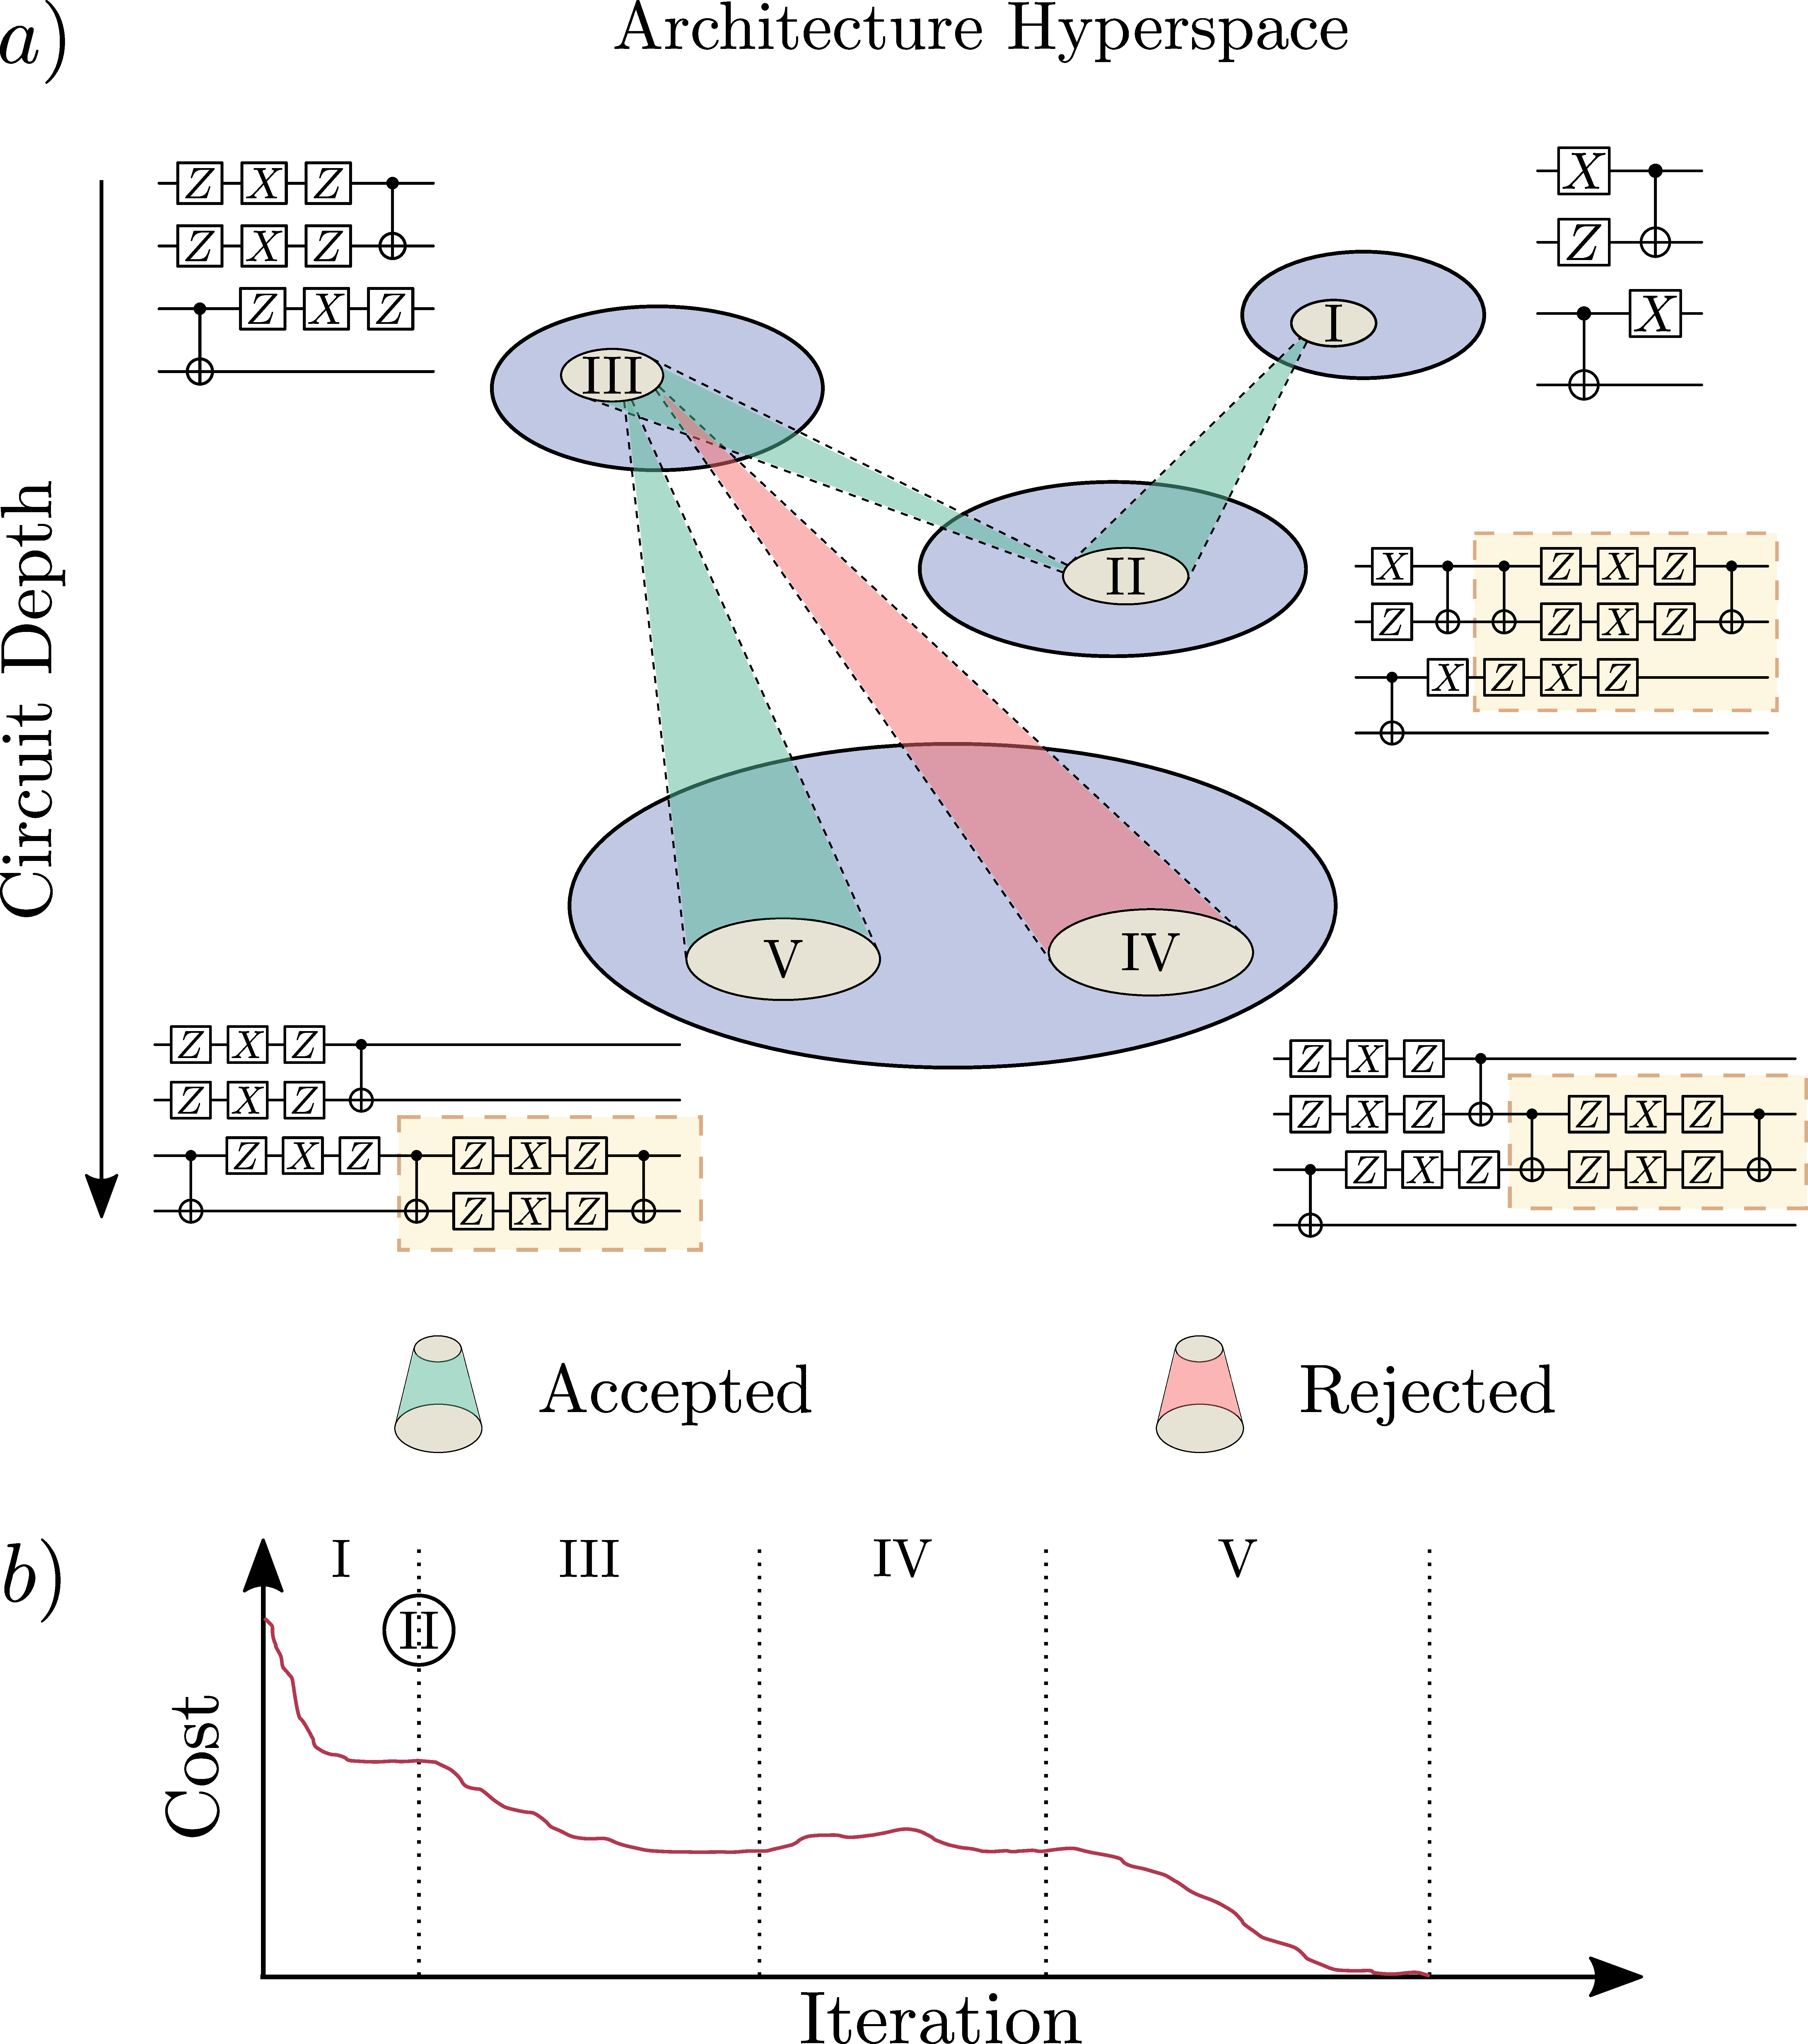
\includegraphics[width=.8\textwidth]{Figures/VANS/Fig1.pdf}
\caption{{\small We show a schematic diagram of the VAns algorithm. \textit{(a)} VAns explores the hyperspace of architectures of parametrized quantum circuits to create short depth ansatzes for VQA applications. VAns takes a (potentially non-trivial) initial circuit (step I) and optimizes its continuous parameters $\thv$ until convergence. At each step, VAns inserts blocks of gates into the circuit which are initialized to the identity (indicated in a box in the figure), so that the ansatzes at contiguous steps belong to an equivalence class of circuits leading to the same cost value (step II). VAns then employs a classical algorithm to simplify the circuit by eliminating gates and finding the shortest circuit (step II to III). The ovals represent subspaces of the architecture hyperspace connected through VAns. While some regions may be smoothly connected by placing identity resolutions, VAns can also explore regions that are not smoothly connected via a gate-simplification process. VAns can either reject (step IV) or accept (step V) modifications in the circuit structure. Here $Z$ ($X$) indicates a rotation about the $z$ ($x$) axis. \textit{(b)} Schematic representation of the cost function value versus the number of iterations for a typical VAns implementation which follows the steps in \textit{(a)}.}}
\label{fig:schematic}
\end{figure}

\afterpage{\clearpage}

To this end, we combine several features of recently proposed methods and introduce the Variable Ansatz (VAns) algorithm~\cite{bilkis2021semi} to generate variable structure ansatzes for generic VQA applications. As shown in Fig.~\ref{fig:schematic}, VAns iteratively grows the parameterized quantum circuit by adding blocks of gates initialized to the identity, but also prevents the circuit from over-growing by removing gates and compressing the circuit at each iteration. In this sense, VAns produces shallow circuits that are more resilient to noise, and that have less trainable parameters to avoid trainability issues. Our approach provides a simple yet effective way to address the ansatz design problem, without resorting to resource-expensive computations similar to recently evolutionary-oriented proposals.

Our algorithm is inspired by the strong presence of noise in NISQ devices. As such, it potentially hinders any successful application of NISQ computers. In this context, we should take advantage of every component of the quantum device that could be optimized over, and this generally includes the circuit's layout. In this regard, some approaches ---as EVQE~\cite{rattew2019domain} or MoG-VQE~\cite{chivilikhin2020mog} ---have been introdued in the past, as discussed in Sec.~\ref{ssec:1_nisq_vans_bp}. VAns algorithm differs from them in at least two important aspects: \textit{(i)} it considers general cost functions, and thus can be considered a general-purposed quantum-machine learning algorithm, and \textit{(ii)} the method incorporates knowledge on quantum computing via specific circuit compression rules.

Thus, the learning problem we are dealing with consists in finding cost-minimizing quantum circuits, where not only the parameters can be optimized, but also the structure of the circuit itself. While some light is shed into the learning problem through the aforementioned compression rules, an important \textit{learning-in-the-darkness} component remains. In particular, no structure is imposed on how our algorithm grows the quantum circuit, and at each time-step quantum gates are randomly placed across the circuit, acting on qubits that are also randomly selected. Thus, the learning paradigm departs from the one considered in Chapter~\ref{chapter:RLCOH}, and rather than assuming complete ignorance of the setting, the agent (VAns algorithm) is now equipped with partial information about the setting, henceforth it learns in the twilight through the VAns algorithm, which we now turn to explain in detail.

\subsection{Bandit problems}\label{ssec:1_rl_bandit}
The multi-armed bandit problem constitutes a simplified version of the RL setting. Here, an agent is faced towards a set of $N$ slot-machines, and each action $a \in \cA= \llaves{1,...,N}$ stands for the pulling arm of the $a$-th machine, which retrieves a reward $r \in \cR$ with an unknown probability $\tau(r|a)$. Each episode starts from a single default state, the bandit can only pull one machine at the episode, which ends right after obtaining the reward; thus the MDP is reduced to a Markov Reward Process (MRP). Though it is not clear who the actual \textit{bandit} is, the situation models a gambler trying to maximize its earnings in a casino. Note also that we restrict to the case in which arms' distributions are stationary, \textit{e.g.} do not change in time.

The bandit problem is ideal to discuss our figures of merit when it comes to model-free learning optimal policies, and in particular to characterize learning curves behaviour. On the one hand, we would like the agent to identify the arm which --- on average --- leads to the highest reward. If the agent knew beforehand all reward distributions $\tau(r|a)$, then it would readily know which action to take. Nevertheless, since no access is granted to those distributions (for otherwise that would be a very generous casino), we then monitor how reward acquisition evolves \textit{during} the learning process. In this regard, a reasonable figure of merit is the cumulative reward
\begin{align}
\Rt(\pi) = \frac{1}{t}\sum_{\nu=1}^t r_\nu
\end{align}
where $r_\nu$ is the reward enjoyed by the agent at episode $\nu$. As such, the cumulative reward is an stochastic quantity, and depends on agent's policy $\pi$ (\textit{i.e.} the way it decides for which arm to sample at a given episode). Whenever it is clear from the context, we will drop the dependence on $\pi$ and simply denote the cumulative reward as $\Rt$. Note that the cumulative reward is upper-bounded (on average) by that one associated to the optimal policy, which always samples from $a^* = \argmax{a\in\cA}Q(a)$, with $Q(a) = \mathbb{E}_r[\tau(r|a)]$. Such expected values $Q(a)$ quantify how \textit{valuable} each action $a$ is, and are the analogue of state-action value functions in MRP --- a slightly more complex quantity that we will define in Sec.~\ref{ssec:1_rl_seqDec} ---. While the agent is not aware of those values, successful learning hinges on how accurately can the agent discriminate between such quantities, and in particular find the optimal one. To this end she updates and estimate of such quantity as new samples are obtained, which we denote by $\hat{Q}(a)$.
% Thus, the closet $\Rt(\pi)$ is, on average, to $\Rt(\pi^*)$, then clo
In particular, bandit theory defines the so-called \textit{expected cumulative regret}:
\begin{equation}\label{eq:CumRegegret}
  \mathcal{L}_t =  \mathbb{E}\big[ \sum_{k=1}^{t} \Big( Q(a^{*}) - Q(a^{(k)}) \Big) \big] = t \;\big(Q(a^{*}) - \mathbb{E}[ \Rt ]\big),
\end{equation}
where $\mathbb{E}$ indicates the expected value with respect to different agents (that experience different realizations of the sampling processes) following the same policy $\pi$,%, but also over the possible conditionings that said strategy $\pi$ requi
and $a^{(t)}$ is the action actually taken by the agent at episode $t$. The cumulative regret is closely related to the (expected) cumulative reward per episode $\Rt$, and quantifies the price to pay, or loss, for taking actions different from the optimal one $a^{*}$. In other words, it quantifies the difference in earnings of the agent with respect to those of a model-aware super-agent, which owns the casino and hence has access to $a^*$.

One of the most fundamental results in bandit theory is the Lai-Robbins bound~\cite{Lai1985} for the asymptotic behaviour of the expected cumulative regret:
\begin{equation}\label{eq:RLBOUND}
 \mathcal{L}_t \underset{t > 1}{\gtrsim} \log t \Big( \sum_{a \in \cA\backslash \{a^{*}\}} \frac{\Delta_a}{\text{KL}(a||*)} + o(1) \Big):=C_{\mathrm{LR}} \log t,
\end{equation}
with $\Delta_a = Q(a^{*}) - Q(a)$ and $\text{KL}(a||*)$ the Kullback-Leibler divergence between the reward distributions $\tau(r|a) $ and $ \tau(r|a^{*})$.
%Recalling the definition in Eq.~\eqref{eq:CumRegegret} we note that the Lai-Robbins bound characterizes the learning curve behaviour in the asymptotic regime: indeed, the average reward over agents, $\mathbb{E}[\Rt]$ can approach the optimal value not faster than $\mathbb{E}[\Rt] \lesssim Q(a^{*})-C_{\mathrm{LR}} \frac{\log t}{t}$.

Recalling that the agent is unaware of the underlying distribution $\tau(r|a)$, we note that $\Rt$ is a figure of merit that detects whether the learning behaviour has improved or not, and is readily available to the agent. In particular, it captures the entire learning process, and measures how well the agent has balanced between exploring potentially optimal (yet undersampled) arms, or exploiting arms that she consider the best, according to the statistics gathered up to episode $t$. Such tradeoff is known as the \textit{exploration-exploitation tradeoff}, and is one of the core concepts in RL theory. It also captures the relevance of bandit problems in real-life applications, where the final success probability of the protocol is not the only figure of merit, but the whole learning process counts. For example, in clinical trials~\cite{Thompson1933} one needs to find the right compromise between advancing in the search of the best treatment (\textit{exploring}) while effectively treating current patients (\textit{exploiting}). Moreover, if one as a scientist is aware of the setting, and aims to monitor the \textit{average} learning behaviour of the agent, the expected regret is readily accessible (provided that enough realisations of the learning process could be simulated), and we know from Lai-Robbins bound that such quantity is assymptotically bounded.
In this regard, the general traits of the cumulative reward per episode $\Rt$ could inspire several ways of quantifying the performance of the learning agent, \textit{e.g.}, \textit{(a)} the onset episode at which $\Rt$ starts exceeding a completely random policy (which samples a random arm unconditioned on the history of past rewards acquired); \textit{(b)} the transient episode at which $\Rt$ reaches a given fraction of its upper bound $\Rt(\pi*)$;  \textit{(c)} the learning speed as quantified by the slope of $\Rt$ after the onset episode; and so on. While little is known on how such traits behave, the expected regret constitutes a route to design policies in bandit problems, which are considered \textit{good} ones if they assimptotically saturate the Lai-Robbins bound. Thus, bandit theory provides us with a framework were some of these notions can be rigorously studied, though extending such formal approach to the general MDP is a challenging task, and constitutes an active area of research~\cite{banditbook, regRL1, regRL2, thesisRegret, QlearningUCB}.%, and one often relies on heuristics (see Sec.~\ref{ssec:rlcoh_dolinar_plus_bandit}).

We will now turn to review some well-known policies that are used in bandit problems, and that will find use in this thesis when dealing with reinforcement learning scenarios (see Sec.~\ref{sec:rl_coh_model_free}).

Recall that at each episode, the agent keeps an estimate $\hat{Q}(a)$ of how valuable taking each action is, by estimating the mean reward it provides. Here, the non-trivial question is which arm to try, given the experience gathered so far. The most straightforward policy to use is the $\epsilon$-greedy, which is outlined in Algorithm~\ref{alg:epgreedybandit}, and consists on going greedy (that is, choosing action $\argmax{a\in\cA}\hat{Q}(a))$ with probability $\epsilon$, or to randomly choose an action with probability $1-\epsilon$. After enjoying the reward, a Monte-Carlo like update is performed on $\hat{Q}(a)$,
which sequentially updates such average value according to some learning-rate $\lambda_t(a)$, and which might depend on both the arm label and the episode number. While small values of $\epsilon$ will favour potentially sub-optimal actions that were discovered by the agent in early episodes, large values of $\epsilon$ imply a random behaviour, and thus a low reward acquisition. In general, the value of $\epsilon$ is modified ah-hoc with the episode number.

\begin{algorithm}[H]\label{alg:epgreedybandit}
  \DontPrintSemicolon
  \SetAlgoNoEnd
  \SetKwInOut{Input}{input}\SetKwInOut{Output}{output}
  \Input{$\hat{Q}(a)$ arbitrarily initialized and learning rates $\lambda_{t}(a) \in (0, 1]$ $\forall a \in \cA\;$, $\epsilon \in (0,1]$}
  \For{ $t$ in $1$ ... $T$  }{
  $\; \; \; \; \; \;$\texttt{generate a random number j}\;
  $\; \; \; \; \; \;$\If{\texttt{j} $\leq \epsilon$}{$\; \; \; \; \; \; \; \; \; \;$\texttt{choose} $a$ \texttt{at random}}$\; \; \; \; \; \;$\Else{}{$\; \; \; \; \; \; \; \; \; \;$\texttt{choose} $a =\argmax{a \in \cA} \hat{Q}(a)$}\;
  $\; \; \; \; \; \;$\texttt{observe} $r$\;
  $\; \; \; \; \; \;$\texttt{update} $\hat{Q}$: \;$\; \; \; \;  \; \; \; \; \; \;\; \; \hat{Q}(a) \leftarrow \hat{Q}(a) + \lambda_{t}(a) [r - \hat{Q}(a)]$
  }
\caption{We detail the $\epsilon$-greedy policy for bandit problems.}
\end{algorithm}
Note that by choosing the learning rates $\lambda_t(a)$ to be the inverse of the number of times action $a$ was visited up to time $t$, then
\begin{equation}
   \hat{Q}(a)  \underset{t \rightarrow \infty}{\rightarrow} \sum_{r \in \cR} r \; \tau(r|a) \; = Q(a) \; \; \forall a \in \cA.
   \label{eq:Qband}
\end{equation}
Moreover, an $\varepsilon$-greedy strategy can not attain the logarithmic behaviour for the $\mathcal{L}_t$ since $\mathbb{E}[ \Rt]<Q(a^{*})$ for all $t$, because at every episode there is a finite probability $\varepsilon$ that the agent performs a suboptimal action, and thus the expected cumulative regret grows linear with $t$. It is then clear that there is room for improvement before saturating the bound in Eq.~\eqref{eq:RLBOUND}.

In what follows we will present two strategies, one based on Upper Confidence Bounds (UCB) ~\cite{Lai1985,Agrawal1995,Auer2002} and the other based on Thompson sampling (TS)~\cite{Thompson1933,Thompson1935,Scott2010,Russo2018}, which substantially improve the performance of $\varepsilon$-greedy and even attains the assymptotic logarithmic behaviour for $\mathcal{L}_t$~\cite{TSoptimal}.% the Lai-Robbins ultimate bound \cite{TSoptimal, Auer2002}.

In UCB, the agent keeps a record of the number of times each action $a$ was selected up to episode $t$, which we denote as $N_{t}(a)$. Hoeffding's inequality bounds the probability that the $\hat{Q}(a)$ underestimates the true value of ${Q}(a)$  by more than $\varepsilon(t)>0$, as
\begin{equation}\label{eq:ucbeq}\small
{\rm Pr}[ \hat{Q}(a)<Q(a)-{\varepsilon}(t) ] \leq e^{- 2 N_{t}(a) {\varepsilon}(t)^{2}} =: \mathcal{P}(t).
\end{equation}
%where here and in the rest of this section we assume that $r\in [0,1]$.
Then, for  $N_{t}(a)>0$, the upper confidence bound, defined as
\begin{equation}\label{eq:ucbeq2}
{\rm ucb}_{t}(a):=\hat{Q}(a)+\varepsilon(t) = \hat{Q}(a)+\sqrt{\frac{-\log \mathcal{P}(t)}{2 N_{t}(a)}} ,
\end{equation}
represents an upper bound to the true value ${Q}(a)$ with a high probability $1-\mathcal{P}(t)$.
This value is used to compare and choose among the different actions, \textit{i.e.}
$a = \argmax{a \in \cA}\mathrm{ucb}_t(a)$, and responds to the motto \textit{optimism under the face of uncertainty}: actions that have not been visited enough are assigned an \textit{optimistic} estimate value and hence more chances of being picked; in addition, actions whose Q-estimate is accurate but sub-optimal will have little chances to be picked again. The functional form of $\mathcal{P}(t)$ can be tuned to balance exploration and exploitation. In particular, for the standard choice $\mathcal{P}(t) = t^{-4}$ it can be proven that the expected cumulative regret $\mathcal{L}_t$ follows the logarithmic scaling ~\cite{Auer2002, banditbook}.

\begin{algorithm}[h]\label{alg:ucbandit}
  \DontPrintSemicolon
  \SetAlgoNoEnd
  \SetKwInOut{Input}{input}\SetKwInOut{Output}{output}
  \Input{$\mathcal{P}(t)$, initialize $\hat{Q}(a), N(a)$ to zero $\forall a \in \cA\;$. }

  \For{$t$ in $1, ...,T$ }{
  $\; \; \; \; \; \;$ \If{ $t \leq \big| \cA \big|$}{
  $\; \; \; \; \; \; \; \; \; \; \; \;$\texttt{(choose each action once)} $a = t$}
  $\; \; \; \; \; \;$ \Else{
  $\; \; \; \; \; \; \; \; \; \; \; \;$
  \texttt{choose} $a = \argmax{a \in \cA} ucb_t(a)$, (Eq.~\eqref{eq:ucbeq2})
  }
  $\; \; \; \; \; \;$ \texttt{observe reward} $r$ \;
  $\; \; \; \; \; \;$ \texttt{record visit: }\;
  $\; \; \; \; \; \; \; \; \; \; \; \; N_t(a)) \leftarrow N_t(a) +1$ \;
  $\; \; \; \; \; \;$ \texttt{update Q-value: } \;
  $\; \; \; \; \; \; \; \; \; \; \; \;  \hat{Q}(a) \leftarrow \hat{Q}(a) + \frac{[r - \hat{Q}(a)]}{N_t(a)}$\;

  }
\caption{UCB for bandit problems.}
\end{algorithm}

Instead of updating an estimate $\hat{Q}(a)$ for each action, in Thompson sampling (TS) a Bayesian approach is followed, where at every episode a full prior distribution (and not just an expectation value) is assigned to the \emph{expected reward} $\bar{r}$ of every arm $a$, $f_{t}(\bar{r}|a) \; \forall a \in \cA$. This distribution characterizes the knowledge the bandit has about the expected earnings of each arm, $Q(a)$, and at the first episode can be taken to be flat over the whole interval $[0,1]$. The policy then consists in sampling an expected reward $\bar{r}\sim f_{t-1}(\bar{r}|a)$
\emph{for each} possible action $a$ and choosing the action with the largest sample $\bar{r}$:
$a=\argmax{a\in\cA}\{\bar{r}\sim f_{t}(\bar{r}|a)\})$; such sampling procedure constitutes an overhead for the bandit, since at each episode $N$ extra samples are required, which are nonetheless unrelated to the arms (\textit{i.e.} at each episode, the bandit still samples only a single arm). Finally, the distribution for the chosen action is updated according to the true reward $r$ obtained, using Bayes' theorem.

\begin{algorithm}[b!]\label{alg:tsber}
  \DontPrintSemicolon
  \SetAlgoNoEnd
  \SetKwInOut{Input}{input}\SetKwInOut{Output}{output}
  \Input{$\mu_1(a), \nu_1(a)$ initialized to one $\forall a \in \cA\;$}
\;
  \For{$t$ in $1, ...,T$ }{
  \;
  $\; \; \; \; \; \;$ \For{ $a$ \texttt{in} $\cA$}{
  $\; \; \; \; \; \; \; \; \; \; \; \;\; \; $\texttt{draw} $\bar{r}_a \texttt{ according to } \text{Beta}(\mu_t(a), \nu_t(a))$} \;
  $\; \; \; \; \; \;$ \texttt{choose} $a = \underset{a}{argmax} \; \bar{r}_a$\;
  $\; \; \; \; \; \;$ \texttt{observe reward} $r$ \;
  $\; \; \; \; \; \;$ \texttt{update Beta distribution: }\;
  $\; \; \; \; \; \; \; \; \; \; \; \;\; \; \mu_{t+1}(a)=\mu_{t}(a) + r$ \;
  $\; \; \; \; \; \; \; \; \; \; \; \;\; \; \nu_{t+1}(a)=\nu_{t}(a) + 1-r$\;
  }
\caption{TS for Bernoulli bandit problems.}
\end{algorithm}

In order to avoid computationally-expensive Bayesian updates, families of distributions that are closed under the update rule are used. In the case of Bernoulli bandits, beta-distributions are employed since those are precisely their conjugate priors. That is, given
\begin{equation}\label{eq:betaDistro}
f_{t}(\bar{r}|a)=\text{Beta}(\mu_t(a), \nu_t(a))\propto \bar{r}^{\mu_{t}(a)-1}(1-\bar{r})^{1-\nu_{t}(a)},
\end{equation}
upon obtaining a reward $r$ the prior is updated to a beta distribution with parameters  $\mu_{t+1}(a)=\mu_{t}(a) + r$, $\nu_{t+1}(a)=\nu_{t}(a) + 1-r$, where at the first episode it is $\mu_{1}(a)=\nu_{1}(a)=1 \;\; \forall a \in \cA$  (flat prior). By mimicking the underlying distributions, TS gauges exploration according to the information acquired so far: if a certain action has not been sampled enough at episode $t$, its reward distribution will still be broad and, when sampled, can easily return a higher value of $\bar r$ than that obtained from other (more peaked) distributions; thereby TS will favour to explore such action. At the same time, if a sub-optimal action has been sampled enough episodes, it will be very unlikely that it is sampled again, since the corresponding prior will be highly peaked at low values. %The pseudo-code of TS for Bernoulli bandits is described in Algorithm~\ref{alg:tsber}.

TS algorithm has been introduced surprisingly long ago~\cite{Thompson1935}, and it is kown to assymptotically attain the Lai-Robbins bound~\cite{regTS1}. Moreover, its performance has been studied in non-assymptotic regimes~\cite{workTSFOLK}, where it was shown that sub-leading constants and terms of order $\log(\log t)$ might be important. Finally, a review about TS and its applicability can be found in Ref.~\cite{Russo2018}.

Let us conclude this overview of bandit theory by introducing the \textit{simple regret}, another widely used figure of merit that quantifies how well has the agent learned to identify the optimal action at episode $t$, regardless of her actual performance:
\begin{equation}
\Lambda_t = \mathbb{E} \big(Q(a^{*}) - Q(a^{(t)*}) \big),
\end{equation}
where $a^{(t)*}$ is the agent's \emph{recommendation} of which the optimal action is at episode $t$. For example, in an $\epsilon$-greedy strategy, the recommendation is given by $a^{(t)*}=\argmax{a}\hat{Q}(a)$. Thus, strategies designed to minimize $\Lambda_t$ will prioritize to learn what the optimal arm to pull is, regardless of the rewards acquired during the entire learning process. %, and the probability that the agent confuses the optimal arm by a sub-optimal one will be exponentially small, hence $\Lambda_t $ will converge to zero exponentially fast.
Recent results~\cite{simpleRegretMunoz} show that the exploitation-exploration trade-off manifests itself in the asymptotic scaling of the simple and cumulative regret in the sense that one imposes lower and upper-bounds on the other, and therefore optimizing one usually affects the performance of the other.

Having gained some intuition on why model-free learning schemes are complex, we will not return to study the general MDP setting.

\subsection{Value functions and the Bellman equation}\label{ssec:1_rl_seqDec}
The complexity added in MDPs, as compared to bandit problems (MRPs), is that agent and environment sequentially interact during (a possibly infinite number of) time-steps. Similar to the bandit case, agent's objective is to acquire as much reward as possible during an episode, and as a matter of fact this strongly depends on the policy that the agent follows. At the end of episode $t$, in which a sequence of tuples %of states, actions, rewards and next states
$\llaves{(s_\ell, a_\ell, r_{\ell+1})}_{\ell = 0}^{L}$ has been experienced (with $s_{L+1}$ a \textit{terminal state}, and $L$ generally varying among different episodes), the agent's performance after each time-step $\ell$ is evaluated using the so-called \textit{return},
\begin{equation} \label{eq:returnGT}
G_{\ell}^{(t)}=\sum_{i=0}^{L-\ell}\gamma^i r_{i+\ell+1}^{(t)},
\end{equation}
which is the weighted sum of rewards obtained at all future time-steps, with a \textit{discount factor} $\gamma\in(0,1]$, weighting more the rewards that are closer in the future. Note that for infinite-horizon MDPs, i.e., $L\rightarrow\infty$, it must hold $\gamma<1$ to ensure that $G_\ell$ remains finite.

By introducing the return, it is straightforward to assign a value to a state $s$ for a given interaction policy $\pi$, via the so-called \textit{state value function}:
% By following interaction policy $\pi$, the value function of state $s$ is defined as
\begin{equation}\label{eq:vFunc}
v_\pi(s)=\mathbb{E}{\pi}[{G_\ell | s_\ell=s}],
\end{equation}
which is the expected return over all possible trajectories that start from state $s$, take actions according to policy $\pi$ and whose dynamics is governed by $\tau$. In other words, the value function measures how convenient it is to visit state $s$ when policy $\pi$ is being followed, and thus provides a route to qualify the goodness of such policy. Note that this quantity is completely determined by the future trajectories accessible from $s$ and hence its dependence on the time-step $\ell$ can have at most the effect of restricting the set of states on which $v_{\pi}(s)$ is supported at that time; we keep this dependence implicit unless otherwise stated. By writing explicitly the expected value for the first future time-step in Eq.~\eqref{eq:vFunc} and then applying the definition of $v$ recursively, it is easy to show that the state-value function satisfies, for any policy, the \textit{Bellman equation}~\cite{Bellman2003}:
\begin{equation}\label{eq:vBell}
v_\pi(s) = \sum_{\substack{ s'\in\cS, r\in\cR\,\\ a\in\cA}}\tau(s',r|s,a)\pi(a|s)\left(r+\gamma v_\pi(s')\right).
\end{equation}
This equation relates the value of a state $s$ with that of its nearest neighbours $s'$, which can be reached with a single action from $s$, and with the corresponding reward obtained by performing such action.

Since value functions assign a score to the policy $\pi$ being followed, a possible route to solve the reinforcement learning problem is that of maximizing state-value functions. Specifically, the optimal policy $\pi^{*}$, maximizes the state-value function for each $s$ and thus represents the \textit{optimal value function}, which satisfies a particular Bellman equation, which is known as the \textit{optimal Bellman equation}:
\begin{align}\label{eq:vBellOp}
v^{*}(s)&:=v_{\pi^*}(s)=\max_\pi v_\pi(s)\\
&=\max_{a\in\cA}\sum_{s'\in\cS,r\in\cR}\tau(s',r|s,a)\left(r+\gamma v^{*}(s')\right).
\end{align}
In an hypothetical situation where optimal value functions are available, an optimal policy can readily be constructed by selecting an action that, from each state, takes the environment towards the next state whose state-value function is the highest. Nevertheless, to do so one needs to have a precise mapping between actions and next-states, an information which is missing if environment dynamics $\tau(s'|s,a)$ is unavailable to the agent.

For this reason, we define the state-action value function (or Q-function, or Q-value) as the expected return when starting from state $s$ and performing action $a$:
\begin{equation}
Q_\pi(s,a) = \mathbb{E}{\pi}\left[G_\ell | s_\ell=s, a_\ell=a\right],
\end{equation}
which is related to the state-value function by $v_\pi(s)=\sum_{a\in\cA} \pi(a|s) Q_\pi(s,a)$. Whenever it is clear from the context we will drop the dependence on the policy $\pi$ for $Q(s,a)$.
Similar to the state value function, by writing explicitly the expected value for the first future time-step, the Bellman equation for state-action value function reads:
\begin{eqnarray}\label{eq:bellqas}
Q_{\pi}(s,a)&=& \sum_{\substack{ s'\in\cS, r\in\cR\,\\ a\in\cA} } \tau(s',r|s,a)(r+\gamma \pi(a'|s')Q_{\pi}(s',a')).\nonumber
\end{eqnarray}

Importantly, the optimal policy $\pi^*$ can also be obtained by maximizing the Q-function, with a corresponding optimal Bellman equation
\begin{eqnarray}\label{eq:qBellOp}
Q^{*}(s,a)&&:=Q_{\pi^*}(s,a)=\max_\pi Q_\pi(s,a)\\
&&=\sum_{s'\in\cS,r\in\cR}\tau(s',r|s,a)(r+\gamma \max_{a'\in\cA}Q^{*}(s',a')).\nonumber
\end{eqnarray}
Note that the state-action value function $Q(s,a)$ provides a natural generalization of the expected reward $Q(a)$ to the case where agent and environment interact sequentially during an episode, where the necessity of defining enivornment states arises. In the latter case, the Bellman equation trivially reduces to only the first term in the right-hand side of Eq.~\ref{eq:vBell}.

We are now in position to understand the complexity of the reinforcement learning problem. While agent and environment begin to interact through some policy $\pi$, state-action value functions are not available to the agent. In turn, several repetitions of such interaction are required in order to  asses which is the relevant subspace of states and actions (recall that environment dynamics $\tau(s',r|s,a)$ might be stochastic). Since the agent can not do better than randomly sampling actions at the beggining of the learning process, she needs to wait a transient time --- which is related to the probability of randomly arriving to a high-reward region of the state-action space --- until some reward signal that might guide the search is experienced. Once obtained a reward signal, a balance between exploring new regions of the state-action space, and to better estimate current state-action value functions should be made. Here, even if an action deterministically maps a state $s$ to a state $s'$, the agent needs several episodes in order to estimate value functions $Q_\pi(s,a)$, since those depend on the accessible region of the state-action space under policy $\pi$, once $s'$ has been reached, as explicited in the Bellman equation of Eq.~\ref{eq:bellqas}. Moreover, such policy should be modified in order to maximize the expected return. Overall, reaching a reasonable balance between exploration and exploitation in such scenarios is certainly challenging, particularly if the agent has resource constraints such as a finite number of episodes available in order to learn a reasonably good policy.

In this regard, while the model-free assumption is strong, it often happens that such agents discover unknown protocols solving the probem at hand. While the solutions found by RL might not be optimal, they can be better than any previously known one. Moreover, the versatily of the reinforcement learning setting (in particular when defining states, actions and rewards) constitutes an extremely appealing tool the discovery of ansatz to problems that are challenging to tackle (or even to model), as we do in Chapter~\ref{chapter:RLCOH}.
%The problem we have introduced is certainly a hard one. While the model-free assumption is strong, it is often customary, since modelling environments can also be a hard task. %Despite of the complexities and issues stressed above, the reinforcement learning community has arrived to a series of outstanding results --- probably in record time, considering how much effort has it take Scientific Community to reach desired goals ---.

In what follows we will detail one out of the --- very many --- algorithms that can be used in order to learn optimal policies in model-free, reinforcement learning scenarios.

%

\subsection{Q-learning}\label{ssec:1_rl_qlearning}
In the model-free setting, the agent not only has to find an optimal policy by exploiting valuable actions, but also needs to characterize the environment in the first place by exploring possibly advantageous configurations. In such a case, the Q-value is quite helpful since it associates a value to the transitions determined by taking action $a$ from state $s$ and following policy $\pi$ thereafter.

Q-learning is an algorithm that can be used to learn optimal policies in a model-free way, and it was first proposed by Watkins \cite{Watkins1989}. This algorothm is often used as a basis for more advanced RL algorithms~\cite{Mnih2013, ddpg}.
It is based on the observation that any Bellman operator, i.e., the operator describing the evolution of a value function as in Eqs.~(\ref{eq:vBell},\ref{eq:vBellOp},\ref{eq:qBellOp}), is contractive~\cite{algsrl}. This implies that, under repeated applications of a Bellman operator, any value function converges to a fixed point, which by construction satisfies the corresponding Bellman equation. Thus, in order to find $Q^{*}(s,a)$, Q-learning turns the optimal Bellman equation for Q, Eq.~\eqref{eq:qBellOp}, into an update rule for $\hat{Q}(s_{\ell},a_{\ell})$, \textit{i.e.}
, the Q-function's estimate available to the agent at a given time-step $\ell$ of any episode $t=1,\cdots,L$.

After an interaction step $s_{\ell}\rightarrow a_{\ell}\rightarrow r_{\ell+1}\rightarrow s_{\ell+1}$ is experienced, the update rule for the Q-estimate is
\begin{align}\label{eq:QLUPDATERULE}
\hat{Q}(s_{\ell}, a_{\ell}) & \leftarrow (1-\lambda_t(s_{\ell},a_{\ell}))\hat{Q}(s_{\ell}, a_{\ell})\\
&+ \lambda_t(s_{\ell},a_{\ell}) \left(r_{\ell+1}  + \gamma \max_{a'\in\cA(s_{\ell+1})}\hat{Q}(s_{\ell+1}, a')\right),
\end{align}
where $\lambda_t(s,a)$ is the learning rate, which depends on the number of times the state-action pair $(s_{\ell},a_{\ell})$ has been visited.
%In case that the state-action pair $(s_\ell, a_{\ell})$ is visited $k$ times during a single episode, the expected return can be estimated using the \textit{first-visit} or the \textit{every-visit} experiences, where in the second case \eqref{eq:QLUPDATERULE} is applied $k$ times during episode $t$ \cite{Sutton2018}.
Note that in order to do the update at each time-step $\ell$, it is only necessary to enjoy the next immediate reward $r_{\ell+1}$ and observe the next state $s_{\ell+1}$; this method thereby allows an on-line learning of the MDP. A pseudo-code of the algorithm can be found below.
%As it turn to be equivalent for our specific setting, in here all updates are done at the end of the episode.

\begin{algorithm}[h]\label{alg:ql}
  \DontPrintSemicolon
  \SetAlgoNoEnd
  \SetKwInOut{Input}{input}\SetKwInOut{Output}{output}
  \Input{$\hat{Q}(s,a)$ \texttt{arbitrarly initialized} $\forall s \in \cS, \; \forall a \in \cA (s)$; \texttt{learning rates} $\lambda_t(s_\ell,a_\ell) \in (0, 1]$, $\epsilon > 0$}
  \Output{$\hat{Q}(s,a) \sim Q^{*}(s,a)$}\;
  \For{ $t$ in $1$ ... $T$  }{
  $\; \; \;$ \texttt{initialize} $ s_0  \; \; \;$ \;
  $\; \; \;$ \For{\texttt{step }$\ell$ \texttt{in episode} $t$}{$\; \; \; \; \; \;$\texttt{take action }$a_\ell$ \texttt{according to }$\pi$ (e.g. $\epsilon$\texttt{-greedy})\; $\; \; \; \; \; \;$\texttt{observe reward }$r_{\ell+1}$\texttt{ and next state }$s_{\ell+1}$ \; $\; \; \; \; \; \;  $\texttt{update }$\hat{Q}(s_\ell, a_\ell)$ \texttt{according to: }\; $ \; \; \; \;  \; \; \; \; \; \; \hat{Q}(s_{\ell}, a_{\ell}) \leftarrow \hat{Q}(s_{\ell}, a_{\ell})  + \lambda (s_\ell, a_{\ell}) [r_{\ell+1} +$\; $\; \; \; \; \; \;  \; \; \; \;  \gamma \max_{a'} \hat{Q}(s_{\ell+1}, a') - \hat{Q}(s_{\ell}, a_{\ell}) ]$\;$\; \; \; \; \; \;$\If{$s_{\ell+1}$\texttt{ is terminal state}}{$\; \; \; \; \; \; \; \; \; \;$ break}$\; \; \; \; \; \;$\Else{}{$\; \; \; \; \; \; \; \; \; \;s_{\ell} \leftarrow s_{\ell+1}$}
  }
}
\caption{Q-learning pseudo-code.}
\end{algorithm}

After a large number $n$ of iterations of the update rule Eq. \eqref{eq:QLUPDATERULE} for all state-action couples, the convergence of the Q-estimate to the optimal Q-function is guaranteed by two general conditions on the learning rate (also known as Robinson conditions)~\cite{Watkins1989,Sutton2018}:
\begin{align}\label{eq:qLConv}
\hat{Q}(s,a)&\underset{k\rightarrow\infty}{\rightarrow}Q^{*}(s,a)\;\,\forall s\in\cS, a\in\cA(s)\\
&\text{ iff }\sum_{t(s,a)}\lambda_{t}(s,a)=\infty,\;\sum_{t(s,a)}\lambda_{t}(s,a)^{2}<\infty,
\end{align}
where the sums are taken over all interactions at which a given state-action couple is visited.
Once the optimal Q-function is obtained, an optimal (deterministic) policy can be constructed by ``going greedy'' with respect to it, i.e., $\pi^{*}(a|s) = \delta(a,\argmax{a\in\cA} Q^{*}(s,a))$ for all $s\in\cS$, where $\delta(x,y)$ is a Kronecker delta.

In RL literatue, Q-learning is classified as an off-policy method~\cite{Sutton2018}, meaning that it learns the state-action values of a \textit{target policy} - in this case the optimal policy - by taking actions according to an \textit{interaction policy}, generally differing from the first one. The standard Q-learning method commits to an $\epsilon$-greedy interaction policy, where with probability $\epsilon$ the agent chooses a random action and otherwise it chooses the greedy action that maximizes the current Q-estimate. However, as we will see in Sec.~\ref{ssec:rlcoh_dolinar_plus_bandit}, more general strategies can be considered, including a clever search as inspired by UCB or TS algorithms.%, where the policy

Moreover, Q-learning is also classified as a tabular method~\cite{Sutton2018}, meaning that it does not approximate or infer the value function of state-actions that have not been visited. In the latter case, it is customary to use an artificial neural network in order to infer the value of the Q-function, and much of the recent success of reinforcement learning algorithms in discovering new protocols for a wide variaty of problems hinges on such networks.

There is a plethora of reinforcement learning algorithms that has been proposed according to specific constraints imposed in the setting, and there is generally no best algorithm; on the contrary --- as it happens in real-life --- the success of an idea generally depends on the context it is carried out. In general, a combination of them needs to be done in order to attain succesful learning and to prove an advantage over state-of-the-art techniques, when tackling a problem from the reinforcement learning perspective. Before closing up this section in reinforcement learning, let us comment on the case where a model of environment dynamics is available to the agent.
%%%

\subsection{Model aware methods}\label{ssec:1_rl_dp}
In the model-aware scenario, the agent has access to the environment dynamics $\tau(s'r | s,a)$. Nonetheless, the question of how to design an optimal policy still holds: while estimating value functions out of samples is no longer required, the agent still needs to solve the Bellman equation in Eq.~\ref{eq:vBell} in order to compute $v_\pi(s)$ for $s\in\cS$. Moreover, the policy optimization challenge remains, and solving it can be highly non-trivial. Such a problem is known as planning~\cite{Sutton2018}, and can be solved for finite-horizon MDPs via dynamic programming methods.

Here we distinguish between two approaches. On the one hand, there is the sequential approach, which exploits the structure of Bellman equation and solves the policy optimization by splitting the global policy optimization into a sequence of smaller optimization problems~\cite{Bellman2003}. On the other hand, iterative approaches can be formulated for the policy optimization problem, such as value and policy iteration algorithms. The latter approach exploits the contractive property of state value function, and are sligthly more general than the methods we consider here, since they can readily be applied in scenarios where  $L$ (the number of time-steps in each episode) is not fixed~\cite{Sutton2018}). In particular, the state value function can be seen as a fixed point of a contractive operator, called the Bellman operator~\cite{AlgorithmsRLCsaba}. While policy iteration algorithms consist on a loop where value functions are estimated through such contractiveness property and a policy is modified in such a way to optimize such values, value iteration algorihtms straightfowardly apply the optimal Bellman operator in order to compute $v^*(s)\; \forall s\in\cS$; more insight can be gained in \href{https://cs.stanford.edu/people/karpathy/reinforcejs/gridworld_dp.html}{this online demonstration}.

In this thesis we restrict to a sequential optimization of the state value, since we will apply RL algorithms to a problem with a well-defined,  sequential structure, namely the calibration of Dolinar receivers. We thus follow the method introduced by Bellman~\cite{Bellman2003}, which makes use of the recursive relation of Eq.~\eqref{eq:vBellOp} to find the optimal policy step by step, and for this we assume that every episode deterministically ends at a fixed time-step $L$, and denote by $v^{*}_{\ell}(s)$ the optimal value function of state $s$ at time-step $\ell$. Here, the so-called \textit{principle of optimality} holds, which is nothing than the optimal value equation in Eq.~\ref{eq:qBellOp}, and states that an optimal policy can be obtained by going greedy sequentially, \textit{e.g.} step by step. Hence, since the optimal policy consists in taking the best possible action from any given state, it can be constructed by concatenating optimal (and local) policies at each time-step: we start by solving Eq.~\eqref{eq:vBellOp} at the last time-step,
\begin{equation}\label{eq:dpL}
v^{*}_{L}(s)=\max_{a\in\cA(s_{L})}\sum_{r\in\cR}\tau(r|s,a)r,
\end{equation}
where we used the fact that $v_{L+1}(s)=0$. The solution to Eq.~\eqref{eq:dpL} provides the optimal action at step $L-1$ for each $s$ and the optimal value function $v^{*}_{L}(s)$.
Then we plug the latter into the optimal Bellman equation for the previous time-step, which in turn can be solved to obtain the optimal action and value function $v^{*}_{L-1}(s)$ for every $s$. By repeating this procedure iteratively for each time-step $\ell=L,\cdots,0$, we can obtain the optimal sequence of actions and value functions for any state at any time-step. This an approach has the nice interpretation of constructing the solution of a large problem by solving smaller problems, each stage essentially adding some complexity into the problem at hand.

The difficulty in this method is that the optimization over actions at a given state \textit{i.e.} $\max_{a\in\cA(s_{\ell})}$ might be find problems. As a matter of fact, we will find difficulties in such optimization landscape when calibrating coherent-state receivers in the presence of noisy channels (see Sec.~\ref{ssec:rlcoh_noise}.)

\subsection{Discussion}\label{ssec:1_rl_discu}
In this section we have introduced some basic concepts in reinforcement learning, which can readily be used by an agnostic agent in order to learn \textit{good} behaviours when acting in unknown environments. The goodness of such behaviours is formally quantified by the amount of reward that the agent gets, on average, when departing from its initial state (or the average over possible states, if there is a non-vanishing probability of the interaction being initialized in more than one state). For this, we have introduced value functions, which are the expected return (\textit{i.e.} a weighted sum of stochastic rewards obtained during an episode) that the agent enjoys when following policy $\pi$, and by doing so we have defined an order relation among policies, \textit{i.e.} a policy $\pi^{'}$ is better than a policy $\pi$ if $v_\pi(s) < v_{\pi^{'}}(s)$ $\forall s\in\cS$. In particular, the agent should seek to perform optimally, and that guarantees her to attain as much rewards as possible, on average, during an episode. We have discussed some methods that the agent can used in order to find such optimal policies, through the optimal state value functions, in Sec.~\ref{ssec:1_rl_dp}. Nonetheless, such methods can only work if a perfect model of the environment dynamics is available to the agent, that is, if the agent knows excatly which is the probability of enjoying a reward $r$, and observe its environment transitioning to state $s'$, when departing from state $s$ and performing action $a$. To gain some intuition on the complexity that model-free scenarios carry on, we have stepped back and discussed a simplified setting in Sec.~\ref{ssec:1_rl_bandit}, known as the multi-armed bandit problem, in which we introduced several strategies that balance between exploring how good untaken actions are, and exploiting potentially sub-optimal yet high-reward-retrieving actions; in particular we studied
$\varepsilon$-greedy, UCB and TS strategies. We then moved to the general MDP case in Sec.~\ref{ssec:1_rl_seqDec}, where the usefulness of the state-action value functions $Q(s,a)$ was highlighted. Finally, we introduced an algorithm that allows the agent to learn optimal policies, called Q-learning, in Sec.~\ref{ssec:1_rl_qlearning}.

These concepts and methods will find use in Ch.~\ref{chapter:RLCOH}, where a reinforcement learning agent is asked to calibrate a quantum receiver out of several repetitions of the experiment. The model-free features of the algorithms we have discussed can readily be used to deal with scenarios where quantum information is transmitted over unknown quantum channels, a result we will present in Sec.~\ref{ssec:rlcoh_noise}. Let us stress that here, even finding sub-optimal strategies might already be a step forward towards better understanding the structure of quantum communication protocols, since little is known about such systems. In this regard, there is plenty of room for the type of machine learning heuristics that are presented along this thesis, in order to help with the development of quantum information protocols. %Thus, even if the reinforcement learning agent gets stuck in sub-optimal policies


